\documentclass[11pt]{report}

\usepackage[a4paper,margin=1in]{geometry}
\usepackage[utf8]{inputenc}
\usepackage[T1]{fontenc}
\usepackage[strings]{underscore}
\usepackage{graphicx}
\usepackage{booktabs}
\usepackage{longtable}
\usepackage{array}
\usepackage{caption}
\usepackage{listings}
\usepackage{xcolor}
\usepackage{hyperref}
\usepackage{amsmath}
\usepackage{enumitem}
\usepackage{tabularx}
\usepackage{fancyhdr}
\usepackage{float}
\usepackage[round,authoryear]{natbib}

\graphicspath{{results/figures/}}
\hypersetup{colorlinks=true, linkcolor=blue, citecolor=blue, urlcolor=blue}

\lstdefinestyle{pystyle}{
  language=Python,
  basicstyle=\ttfamily\footnotesize,
  keywordstyle=\color{blue},
  commentstyle=\color{gray},
  stringstyle=\color{teal},
  numbers=left,
  numberstyle=\tiny\color{gray},
  breaklines=true,
  breakatwhitespace=false,
  frame=single,
  showstringspaces=false,
  tabsize=4,
  columns=flexible,
}
\lstset{style=pystyle}

\pagestyle{fancy}
\fancyhf{}
\fancyhead[L]{DEAP Comparative Analysis: Project Report}
\fancyhead[R]{\thepage}

\title{DEAP EEG Emotion Recognition: A Comparative Analysis of\\
Classical and Deep Learning Pipelines\\
\large Project Report: Methods, Results, Literature Review,\\
and Findings}
\author{Koustav Das}
\date{\today}

\begin{document}

\maketitle
\tableofcontents
\listoffigures
\listoftables

\chapter{Introduction and Objectives}

\section{Purpose of this report}
This document is a technical record of the work I carried out in this
repository: a head-to-head comparison of two feature/modeling paradigms for
binary emotion classification on the DEAP dataset, followed by an extended
investigation into why subject-independent performance on this dataset is
weak, and a final cross-corpus validation against SEED-IV. I wrote it so it
can be expanded into a formal report or thesis chapter: the methods, the
results, every literature source I consulted, and every open item are
documented here in enough detail to reconstruct the reasoning behind each
design decision.

\section{Objectives}
\begin{enumerate}
  \item I built two parallel, directly-comparable pipelines for classifying
        DEAP's four emotion dimensions (valence, arousal, dominance, liking)
        from EEG: a classical-ML pipeline on hand-crafted Differential
        Entropy (DE) band-power features (Track A), and a
        deep-learning pipeline on raw, baseline-normalized EEG windows
        (Track B).
  \item I evaluated both under a subject-independent
        protocol (\texttt{GroupKFold} / \texttt{GroupShuffleSplit}, grouped
        by subject) rather than the leakier, ungrouped splits common in the
        published literature.
  \item Since subject-independent performance turned out to be weak, I
        tested plausible causes one at a time: feature richness,
        hyperparameter tuning, CV rigor, data quantity (window overlap),
        label definition, per-subject calibration, feature/distribution
        alignment, adversarial subject-invariance, self-supervised
        pretraining, an AUC-targeted loss, test-time adaptation, and
        diagnostic interpretability (SHAP).
  \item I checked whether the resulting near-chance ceiling is a property of
        DEAP specifically, or of subject-independent EEG emotion decoding in
        general, via cross-corpus transfer to a second dataset (SEED-IV).
  \item I grounded the design choices above in a review of 32 papers
        (\texttt{papers\_EEG/}) and report every case where an intervention
        did not help.
\end{enumerate}

\section{How this report is organised}
Chapter~\ref{ch:dataset} describes the DEAP dataset and the two evaluation
datasets involved (DEAP itself and SEED-IV). Chapter~\ref{ch:repo} maps the
repository layout. Chapter~\ref{ch:notebook} is the core of the report: the
methods behind each experiment, the results, and a discussion, covering the
main notebook (\texttt{DEAP\_Comparative\_Analysis.ipynb}) end to end.
Chapter~\ref{ch:scripts} is an appendix documenting every standalone
\texttt{scripts/*.py} file and the lower-level implementation detail (function
names, cache file names) that the main chapter omits. Chapter~\ref{ch:literature}
is the literature review and bibliography. Chapter~\ref{ch:results}
consolidates the numeric results into one master table. Chapters~\ref{ch:done}--\ref{ch:challenges}
cover what was accomplished, what was left undone, what I would do
differently, and the concrete challenges I ran into. Chapter~\ref{ch:conclusion}
concludes.

\chapter{Dataset and Problem Setup}
\label{ch:dataset}

\section{DEAP}
The DEAP dataset \citep{koelstra2012deap} (\texttt{data\_preprocessed\_python}) contains 32 subjects
$\times$ 40 trials $\times$ 32 EEG channels sampled at 128\,Hz. Each subject
file \texttt{sXX.dat} is a pickled dictionary with:
\begin{itemize}
  \item \texttt{data}: shape $(40, 40, 8064)$: 40 trials, the first 32 of
        40 channels are EEG (the remaining 8 are peripheral physiological
        signals, dropped throughout this project). 8064 samples = 3\,s
        pre-trial baseline (384 samples) + 60\,s of stimulus (7680 samples).
  \item \texttt{labels}: shape $(40, 4)$: continuous 1--9 self-assessment
        ratings for valence, arousal, dominance, and liking.
\end{itemize}
Labels are binarised at the DEAP-standard threshold of 5.0 (rating $>5 \Rightarrow$
class 1). Section~\ref{sec:s4} shows this binarisation is not
balanced: valence is 21.0\%/79.0\%, arousal 23.3\%/76.7\%, dominance
60.9\%/39.1\%, and liking 66.5\%/33.5\% high/low, a fact that explains a large
share of the most important finding in this report (Section~\ref{sec:s8}).

\section{SEED-IV}
SEED-IV \citep{zheng2018emotionmeter} (``EmotionMeter'') is used as the
cross-corpus validation target in Section~\ref{sec:s12}. It shares SEED's
62-channel montage and 15 subjects, but differs from the original 3-class
SEED dataset in several respects that required a dedicated adapter
(Section~\ref{sec:seed-iv-adapter}): 4 emotion classes (0 = neutral,
1 = sad, 2 = fear, 3 = happy) instead of 3; 24 film-clip trials per session
instead of 15; 3 sessions per subject, each with its \emph{own} trial-label
order (unlike original SEED's single shared label file); and raw trials of
variable duration (tens of thousands of samples at 200\,Hz) rather than
DEAP's fixed 60\,s. I chose SEED-IV over original SEED
because it is mirrored on Kaggle
(\url{https://www.kaggle.com/datasets/phhasian0710/seed-iv}) without a
signed data-use agreement, whereas original SEED, DREAMER, and AMIGOS all
remain gated behind such agreements (see Chapter~\ref{ch:not-done}).

\chapter{Repository Structure}
\label{ch:repo}

\begin{verbatim}
.
|-- README.md                         (dataset links, repo layout, quick start)
|-- Project_Report.tex / .pdf         (this report)
|-- DEAP_Comparative_Analysis.ipynb   (the main notebook)
|-- script_notebook_execution_map.txt (script<->notebook run-order/dependency map)
|-- citations.txt                     (flat paper citation list)
|-- literature_log.txt                (per-paper attribution/summary log)
|-- deap-dataset\data_preprocessed_python\   (raw DEAP .dat files, 32 subjects)
|-- seed-dataset\                     (SEED-IV download: eeg_raw_data/{1,2,3}/, etc.)
|-- processed_cache\                  (cached .npz feature/window builds)
|-- results\
|   |-- tables\   (21 CSV result tables)
|   \-- figures\  (24 PNG figures)
|-- papers_EEG\   (32 literature-review PDFs, renamed to descriptive titles)
\-- scripts\
    |-- dl_models.py, rich_features.py
    |-- build_extended_features.py, build_overlap_windows.py, build_raw_ratings.py
    |-- track_a_*.py   (9 classical-ML companion experiments)
    |-- track_b_*.py   (5 deep-learning companion experiments)
    \-- cross_corpus\
        |-- base.py, seed_adapter.py, run_cross_corpus.py, README.md
\end{verbatim}

The notebook is the primary deliverable; the \texttt{scripts/} directory holds
every experiment that was too expensive to run inline, each of which writes
its results to a CSV in \texttt{results/tables/}, which the notebook then
reads and plots. This split is discussed further in Chapter~\ref{ch:challenges}.
A handful of one-off scripts used to author the notebook's own cells during
earlier stages of the project are not listed above; they are not part of the
reproducible-results path. \texttt{script\_notebook\_execution\_map.txt}, at
the repository root, is the authoritative statement of that split: for every
companion script it names the notebook section and cell range that consumes
its output, the cache file it depends on, and the run order needed to
reproduce every table and figure in this report from a clean checkout;
Section~\ref{sec:execution-map} in the Appendix summarises it.

\chapter{Methods, Results, and Discussion}
\label{ch:notebook}

This chapter covers the main notebook (\texttt{DEAP\_Comparative\_Analysis.ipynb})
end to end: what I did, what I found, and what I make of it. It is organised
by experiment, in the order I ran them, each with its own methods and
results; a single Discussion section at the end synthesises all of them.
Lower-level implementation detail, function names, and cache file names are
in Appendix~\ref{ch:scripts} rather than here.

Reproducibility: \texttt{SEED = 42} fixes randomness in
scikit-learn/XGBoost/PyTorch/NumPy throughout. The notebook runs end to end
without errors in about 16 minutes on the hardware described below.

\section{Data and preprocessing}
\label{sec:s1}
Data loading, feature extraction, and the deep-learning pipeline use
\texttt{numpy}, \texttt{pandas}, \texttt{scipy.signal}, \texttt{scikit-learn}
\citep{pedregosa2011sklearn}
(\texttt{GroupKFold}/\texttt{GroupShuffleSplit}), \texttt{xgboost}
\citep{chen2016xgboost}, and \texttt{PyTorch} \citep{paszke2019pytorch}, run
on an NVIDIA GeForce RTX 3070 Ti. Windows are 4\,s
(\texttt{WINDOW\_SEC = 4}), giving 15 non-overlapping windows per 60\,s
trial; the four spectral bands are theta (4--8\,Hz), alpha (8--13\,Hz), beta
(13--30\,Hz), and gamma (30--45\,Hz); the label threshold is 5.0 on DEAP's
1--9 scale. All 32 subjects were used in every run. Both the window length
and the band edges follow the conventions used across most of the DEAP
emotion-recognition literature I reviewed (Chapter~\ref{ch:literature}),
which keeps the numbers in this report comparable to published work rather
than an artefact of an idiosyncratic preprocessing choice: a wildly
different window length or band definition would make any AUC comparison,
including the leaky-split contrast in Section~\ref{sec:s13}, an
apples-to-oranges one.

Each subject's trial is first baseline-corrected: the per-channel mean of
the 3\,s pre-trial baseline is subtracted from the 60\,s stimulus signal,
removing subject/session DC offset and slow drift before either feature
branch is computed. Skipping this step would let a classifier partly exploit
each subject's idiosyncratic DC offset or electrode-impedance level rather
than a genuine stimulus-driven signal, which would be a confound baked into
every downstream number rather than a real finding. From the
baseline-corrected signal, two parallel representations are built:
\begin{itemize}
  \item \textbf{Differential Entropy (DE) features}, for Track A: a 4th-order
        Butterworth \citep{butterworth1930filter} zero-phase filter splits
        the signal into the four bands above, each band is cut into 15
        non-overlapping 512-sample windows, and the Differential Entropy of
        each (channel, band) pair is computed as $\text{DE} = 0.5 \log(2\pi
        e \, \sigma^2)$, the closed-form differential entropy of a Gaussian
        with the window's own variance $\sigma^2$. This gives 32 channels
        $\times$ 4 bands = 128 features per window. I used Differential
        Entropy rather than raw band power because it is the dominant
        hand-crafted feature in the EEG emotion-recognition literature
        \citep{duan2013differential}, shown in that original work to
        outperform simple band energy on exactly this kind of task, which
        makes Track A a direct test of the field's default feature choice
        rather than a feature I invented for this project. A zero-phase
        (forward-backward) filter is used specifically so that filtering
        does not shift each band's energy in time relative to the other
        bands, which would otherwise distort the Differential Entropy
        computed from a fixed 512-sample window.
  \item \textbf{Raw windows}, for Track B: the same 512-sample windows kept
        in their raw $(32, 512)$ form and standardised per channel (zero
        mean, unit variance within that window) for stable CNN input.
        Per-channel standardisation matters here because raw EEG amplitude
        varies by an order of magnitude or more across subjects and
        recording sessions due to electrode impedance and skull thickness;
        without it, a convolutional filter's learned weights would need to
        simultaneously represent amplitude scale and signal shape, which
        empirically destabilises training far more than it does for
        vision-style inputs with a fixed, known dynamic range.
\end{itemize}
Looping this over all 32 subjects $\times$ 40 trials gives 19{,}200 windows
total: a DE feature matrix, a raw-window tensor, one binary label array per
task, and a subject-ID array used to group folds by subject so no subject's
windows appear in both train and test. Results are cached to disk so
repeated runs do not have to reprocess the raw files. Building both
representations from the same baseline-corrected, windowed signal, rather
than deriving Track B's windows independently, is what makes the Track A
versus Track B comparison in Section~\ref{sec:s7} a comparison of modelling
paradigm rather than of two different, incommensurable preprocessing
pipelines.

\section{Class balance}
\label{sec:s4}
Class counts per task, computed directly from the window array: valence
21.0\% high, arousal 23.3\% high, dominance 60.9\% high, liking 66.5\% high.
Valence and arousal are markedly imbalanced; dominance and liking are closer
to balanced. This imbalance has to be checked before trusting any raw
accuracy number, and it turns out to matter for most of the results in this
chapter.

I ran this check, and put it before any model results rather than after,
because accuracy alone is a misleading metric under class imbalance: a
classifier that always predicts the majority class on valence would already
score 79.0\% accuracy while having learned nothing about the actual signal,
and a reader who saw only an accuracy number for valence with no class-count
context beside it would have no way to tell that classifier apart from a
genuinely discriminative one. \citet{khan_ndreviewfailures} document exactly
this failure mode recurring across published DEAP work, where headline
accuracy numbers survive peer review without a class-balance caveat attached
even though the underlying labels are known to be skewed; checking and
reporting this up front is a direct response to that documented gap, not a
routine formality. ROC-AUC, threshold-independent and insensitive to class
proportions by construction, is used as the primary metric throughout the
rest of this report for exactly this reason, with accuracy reported
alongside it only as a secondary, easily-misread number. The practical
consequence appears repeatedly later in this chapter: Track B's 83.5\%
valence accuracy (Section~\ref{sec:s6}) sits within a few points of the
79.0\% majority-class baseline established here, which is the first concrete
instance of the accuracy/AUC divergence that Section~\ref{sec:s8} discusses
at length and that recurs across nearly every high-capacity model in
Chapter~\ref{ch:model-analysis}.

\begin{figure}[H]
\centering
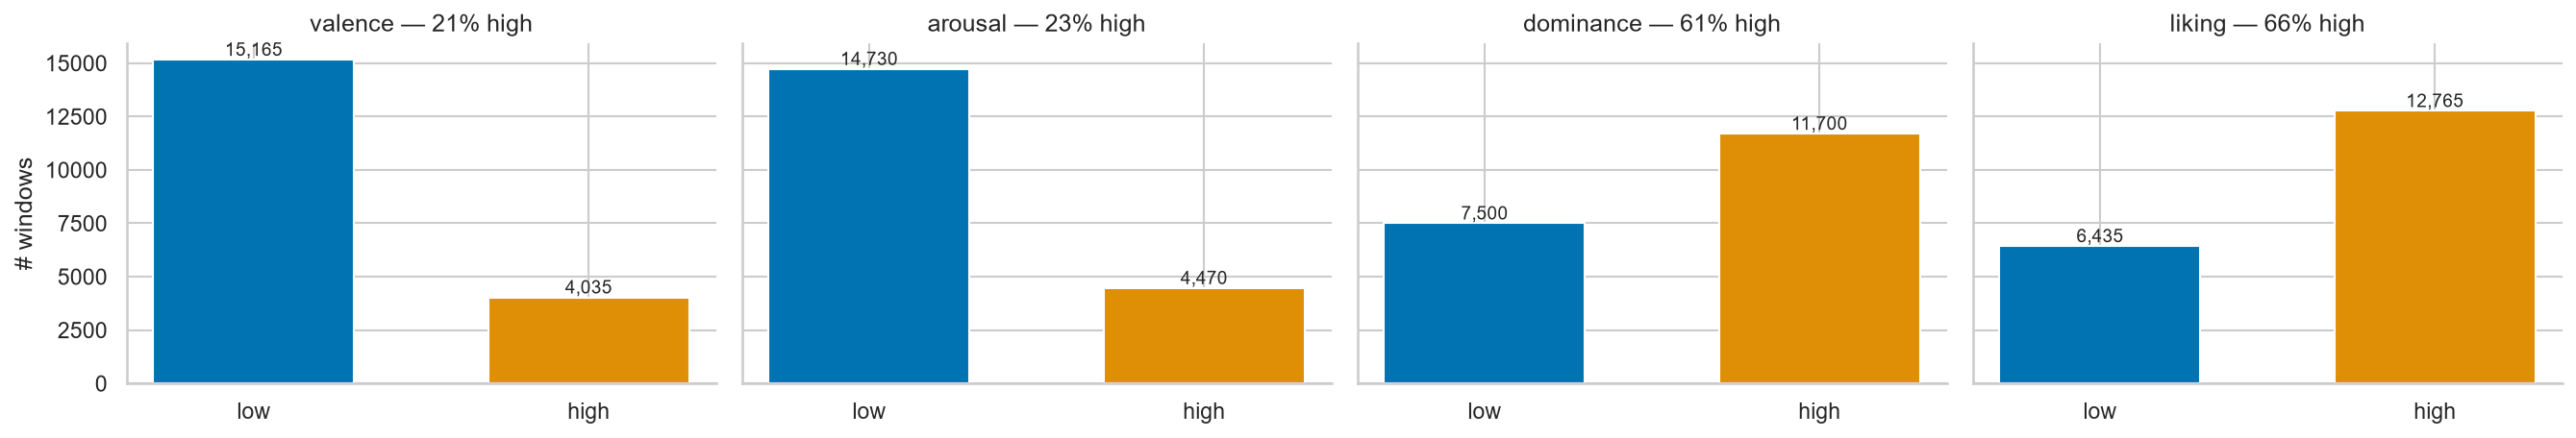
\includegraphics[width=0.8\textwidth]{class_balance.png}
\caption{High/low class balance per task. Valence and arousal are markedly
skewed (21.0\%/79.0\% and 23.3\%/76.7\% high); dominance and liking are
closer to balanced.}
\label{fig:class-balance}
\end{figure}

\section{Track A: classical models on DE features}
\label{sec:s5}
Six models (Logistic Regression, kNN \citep{cover1967knn}, Random Forest
\citep{breiman2001randomforest}, SVM-RBF \citep{cortes1995svm}, XGBoost
\citep{chen2016xgboost}, MLP), each wrapped in a standard-scaling pipeline,
evaluated with 5-fold \texttt{GroupKFold} (grouped by subject, so no
subject's windows appear in both train and test). SVM-RBF's training folds
are capped at 8000 samples, a pragmatic speed trade-off that does not apply
to the other five models.

I chose these six specifically to span as many different inductive biases as
a classical-ML comparison reasonably can on the same 128-dimensional
Differential Entropy input: a linear hyperplane (Logistic Regression), a
non-parametric distance vote with no training-time optimisation (kNN), two
tree ensembles built from opposite objectives -- bagging independent trees
to reduce variance (Random Forest) versus boosting trees sequentially
against residual error (XGBoost) -- a kernel method that can represent a
nonlinear decision boundary without an explicit feature map (SVM-RBF), and a
generic trainable nonlinear function approximator (the MLP). The reason this
breadth matters methodologically, not just descriptively, is made explicit
in Chapter~\ref{ch:model-analysis}: because every one of these six model
families, plus four structurally distinct deep architectures in Track B,
converges on the same narrow AUC band, the breadth of model choice here is
what rules out ``a weak model family was picked'' as an explanation for that
finding. \texttt{GroupKFold}, grouped by subject rather than left ungrouped,
is the single design choice most responsible for how low these numbers are
relative to prior published work on this dataset (Section~\ref{sec:s13}
quantifies the gap directly); it was chosen over an ungrouped split
specifically because an ungrouped split lets windows from the same subject
appear in both the training and test folds, which lets a classifier partly
learn to recognise the subject rather than the emotion, inflating reported
accuracy in a way that would not generalise to a genuinely new user.
Table~\ref{tab:track-a-best} shows the best model per task by ROC-AUC.

\begin{table}[h]
\centering
\caption{Track A: best classical model per task (5-fold GroupKFold mean)}
\label{tab:track-a-best}
\begin{tabular}{lllrrr}
\toprule
Task & Best model (by AUC) & Accuracy & F1 (macro) & ROC-AUC \\
\midrule
valence   & RandomForest & 0.779 & 0.446 & 0.501 \\
arousal   & kNN          & 0.744 & 0.451 & 0.495 \\
dominance & SVM-RBF      & 0.557 & 0.498 & 0.513 \\
liking    & SVM-RBF      & 0.587 & 0.517 & 0.534 \\
\bottomrule
\end{tabular}
\end{table}

\begin{figure}[H]
\centering
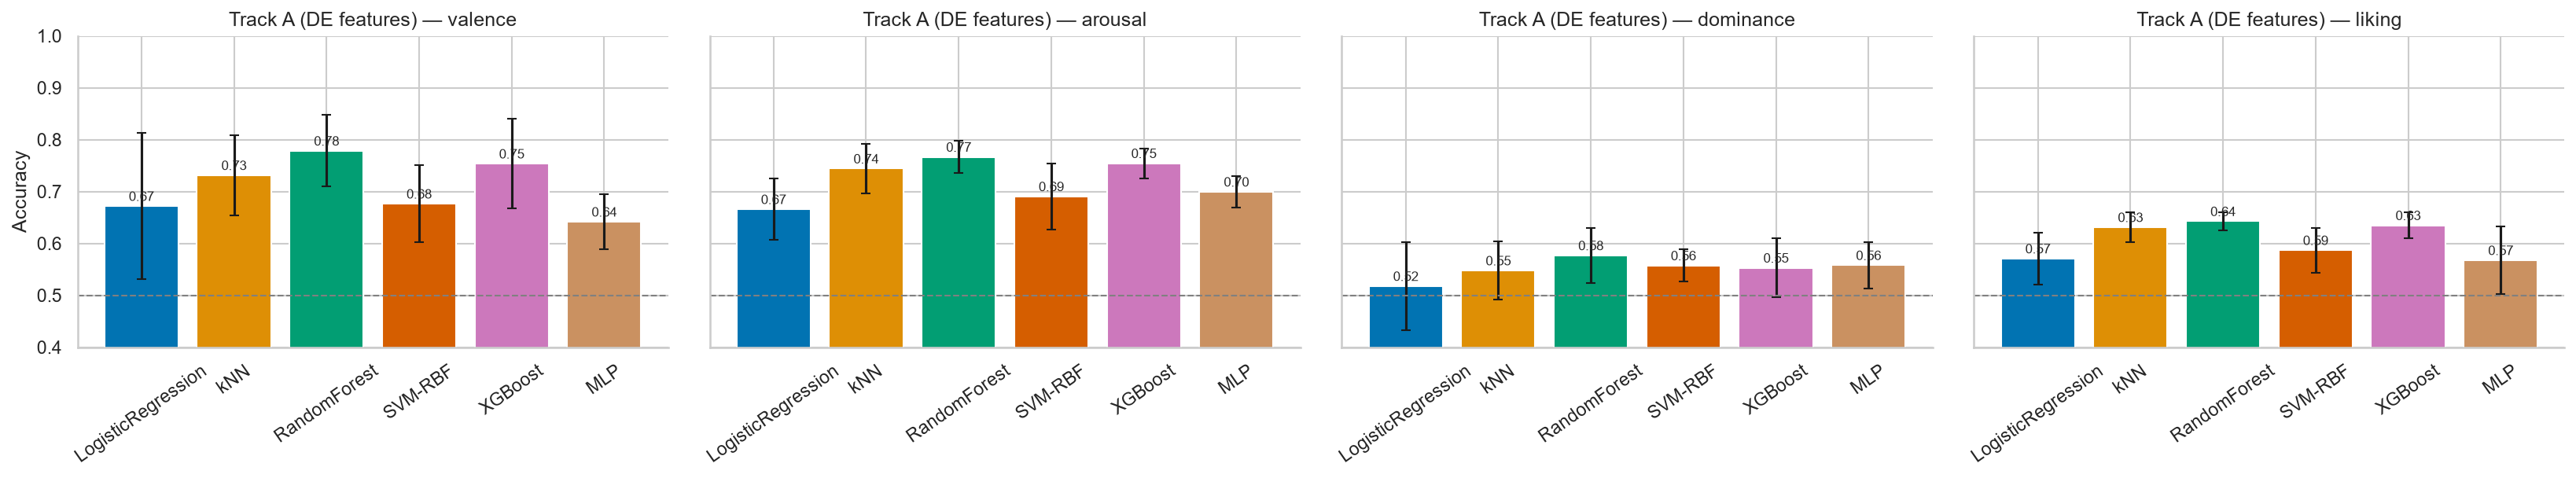
\includegraphics[width=0.85\textwidth]{track_a_accuracy.png}
\caption{Track A: accuracy/F1/ROC-AUC for all six classical models across
all four tasks (5-fold GroupKFold).}
\label{fig:track-a-accuracy}
\end{figure}

\section{Track B: deep models on raw EEG windows}
\label{sec:s6}

\subsection{Model architectures}
Four architectures, all implemented from scratch in PyTorch:
\begin{itemize}
  \item EEGNet \citep{lawhern2018eegnet} (2130 params): temporal conv, then
        depthwise spatial conv, then separable conv, purpose-built for EEG.
  \item ShallowConvNet \citep{schirrmeister2017shallow} (54{,}562 params):
        temporal conv, then spatial conv, then a square/log-power
        nonlinearity, inspired by FBCSP-style band-power features.
  \item CNN-LSTM (82{,}466 params): a spatial-temporal CNN front end
        collapses the channel dimension; a bidirectional LSTM then models
        the resulting temporal sequence.
  \item TSception \citep{ding2022tsception} (8765 params): multi-scale temporal
        ``inception'' branches at three kernel sizes, fused with a global
        spatial conv and a hemisphere-asymmetry spatial conv using DEAP's
        standard channel order. This is a simplified reimplementation in the
        spirit of the original, not a line-for-line port of its codebase.
\end{itemize}
These four were chosen to mirror Track A's spread of inductive biases inside
the deep-learning paradigm: EEGNet and ShallowConvNet are the two most-cited
purpose-built EEG architectures in the literature I reviewed
(Chapter~\ref{ch:literature}), giving Track B a literature-grounded floor
analogous to Track A's use of a standard hand-crafted feature; CNN-LSTM adds
an explicit sequence-modelling component that neither purpose-built
architecture has, to test whether within-window temporal dynamics carry
information a purely spatial/spectral model would discard; and TSception is
included specifically because it hard-codes a named neurophysiological
hypothesis (hemisphere asymmetry) into its architecture, which lets
Chapter~\ref{ch:model-analysis} test whether encoding that hypothesis
structurally helps, rather than assuming it does. Implementing all four from
scratch, instead of importing each paper's reference implementation, was
necessary because none of the original codebases targets this project's
exact input shape (32 channels, 512 samples, DEAP's own channel ordering) or
label set, and it makes every layer of every model auditable against the
architecture described in its source paper rather than trusted as an opaque
dependency.

\subsection{Training procedure}
Each model is trained under a subject-independent 70/15/15 train/val/test
split by subject, so no subject's data crosses a split boundary. Training
uses AdamW \citep{loshchilov2019adamw} with a plateau learning-rate
schedule, automatic mixed precision on the GPU, and early stopping on
validation loss (patience 8, max 40 epochs), restoring the best
validation-loss checkpoint before final test evaluation. AdamW was chosen
over plain Adam because its decoupled weight decay does not interact with
the adaptive per-parameter learning rate the way Adam's coupled $L_2$
penalty does, which matters more than usual here given how small some of
these networks are (EEGNet has only 2130 parameters): an entangled weight
decay term can dominate the update for a parameter with a large adaptive
learning rate, effectively over-regularising exactly the filters a small
network can least afford to lose capacity in. Early stopping on validation
loss, rather than training for a fixed number of epochs, guards against
overfitting to a training fold's particular mix of subjects; given how few
distinct subjects populate each fold (Section~\ref{sec:ma-shared}), a model
trained to convergence without this safeguard would have every opportunity
to memorise subject-specific noise in the training set rather than a signal
that generalises to the held-out subjects.

\subsection{Results: all four models on all four tasks}
16 training runs (4 architectures $\times$ 4 tasks), one train/val/test
split each, on the GPU. Table~\ref{tab:track-b-best} shows the best model
per task.

\begin{table}[h]
\centering
\caption{Track B: best deep model per task (single subject-independent split)}
\label{tab:track-b-best}
\begin{tabular}{lllrrr}
\toprule
Task & Best model (by AUC) & Accuracy & F1 (macro) & ROC-AUC \\
\midrule
valence   & EEGNet     & 0.835 & 0.455 & 0.561 \\
arousal   & EEGNet     & 0.699 & 0.572 & 0.607 \\
dominance & TSception  & 0.589 & 0.414 & 0.475 \\
liking    & CNN-LSTM   & 0.599 & 0.384 & 0.497 \\
\bottomrule
\end{tabular}
\end{table}

Dominance/EEGNet posts AUC 0.288, below chance and the single worst result
in either track. It is an early instance of the arousal/dominance
instability pattern that recurs throughout Sections~\ref{sec:s16} and
\ref{sec:s17}.

\begin{figure}[H]
\centering
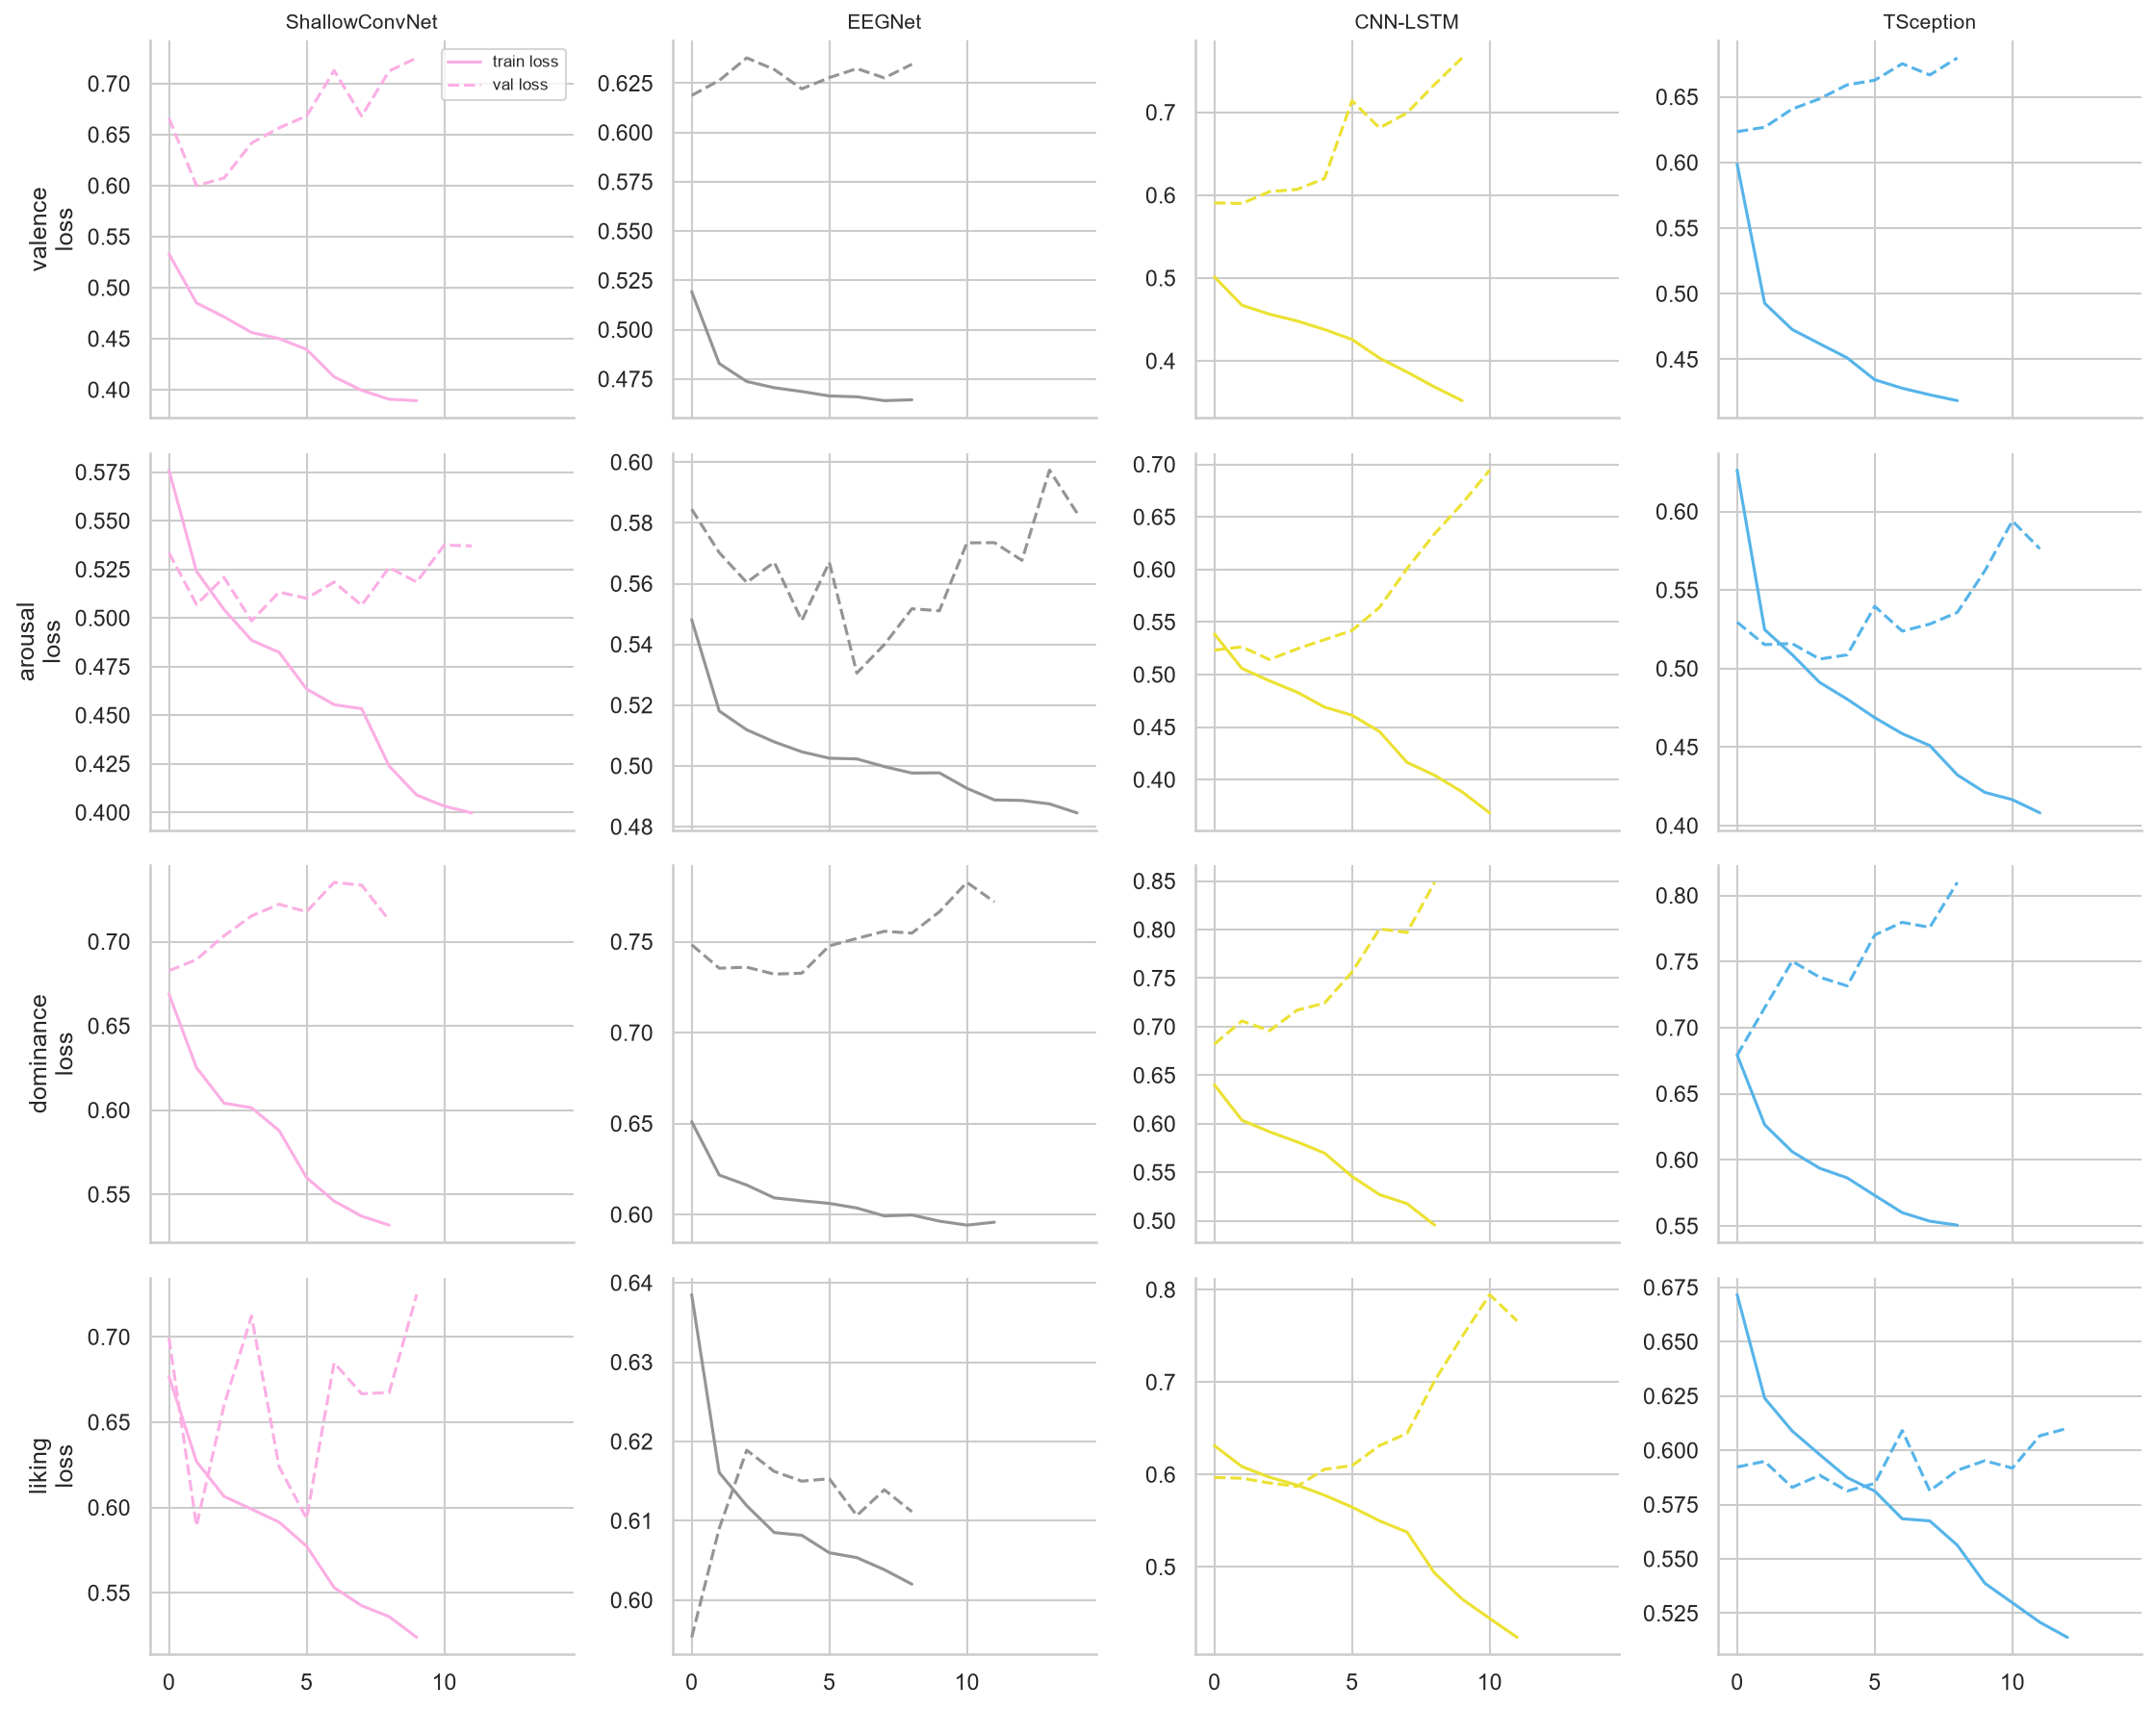
\includegraphics[width=0.9\textwidth]{track_b_training_curves.png}
\caption{Track B: training/validation loss curves for all 16 runs
(4 architectures $\times$ 4 tasks), showing early-stopping behaviour under
the patience-8 schedule.}
\label{fig:track-b-training-curves}
\end{figure}

\section{Combined comparative analysis}
\label{sec:s7}
Track A and Track B results are concatenated into a single 10-model table
and plotted side by side (accuracy/F1/AUC across all 10 models $\times$ 4
tasks), alongside confusion matrices for the model with the highest mean
accuracy on each task.

This step exists because Sections~\ref{sec:s5} and \ref{sec:s6} report Track
A and Track B separately, which makes it easy to compare models within a
track but not across the two paradigms the whole project is built to
compare. Putting all ten models side by side on the same axes, for the same
four tasks, is what turns two separate result sections into the direct
answer to this report's central question (Chapter~\ref{ch:notebook}'s
opening objective): does hand-crafted-feature-plus-classical-ML or
end-to-end deep learning perform better on subject-independent DEAP emotion
classification? A reader should use this section's figures to check, for
each task, which of the ten bars is tallest by AUC (not by accuracy, given
Section~\ref{sec:s4}'s imbalance caveat), and whether that winner comes from
Track A or Track B; Section~\ref{sec:s8} draws out what that comparison
actually shows once class imbalance is accounted for.

\begin{figure}[H]
\centering
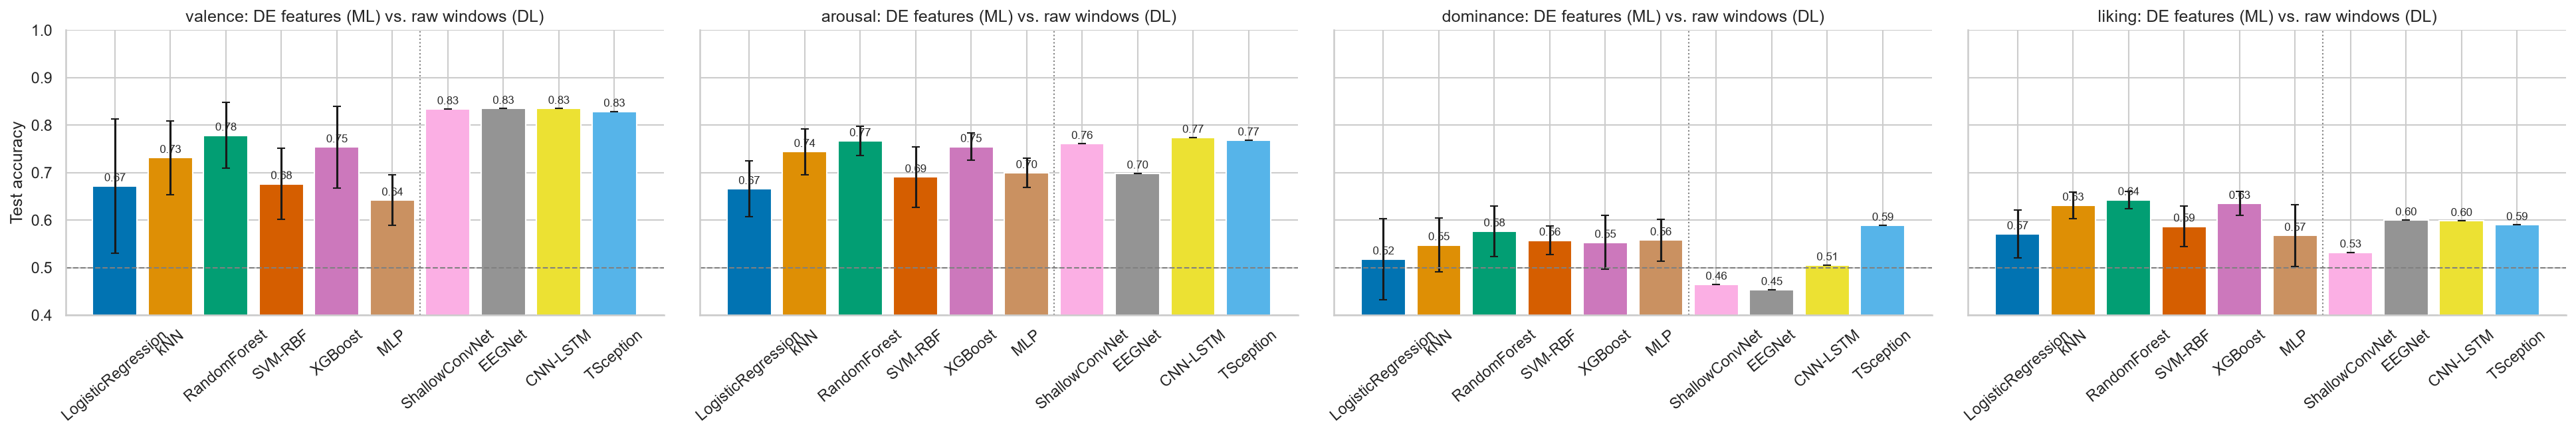
\includegraphics[width=0.9\textwidth]{combined_accuracy_comparison.png}
\caption{Combined accuracy/F1/ROC-AUC comparison across all 10 models
(6 classical + 4 deep) and all 4 tasks.}
\label{fig:combined-accuracy}
\end{figure}

\begin{figure}[H]
\centering
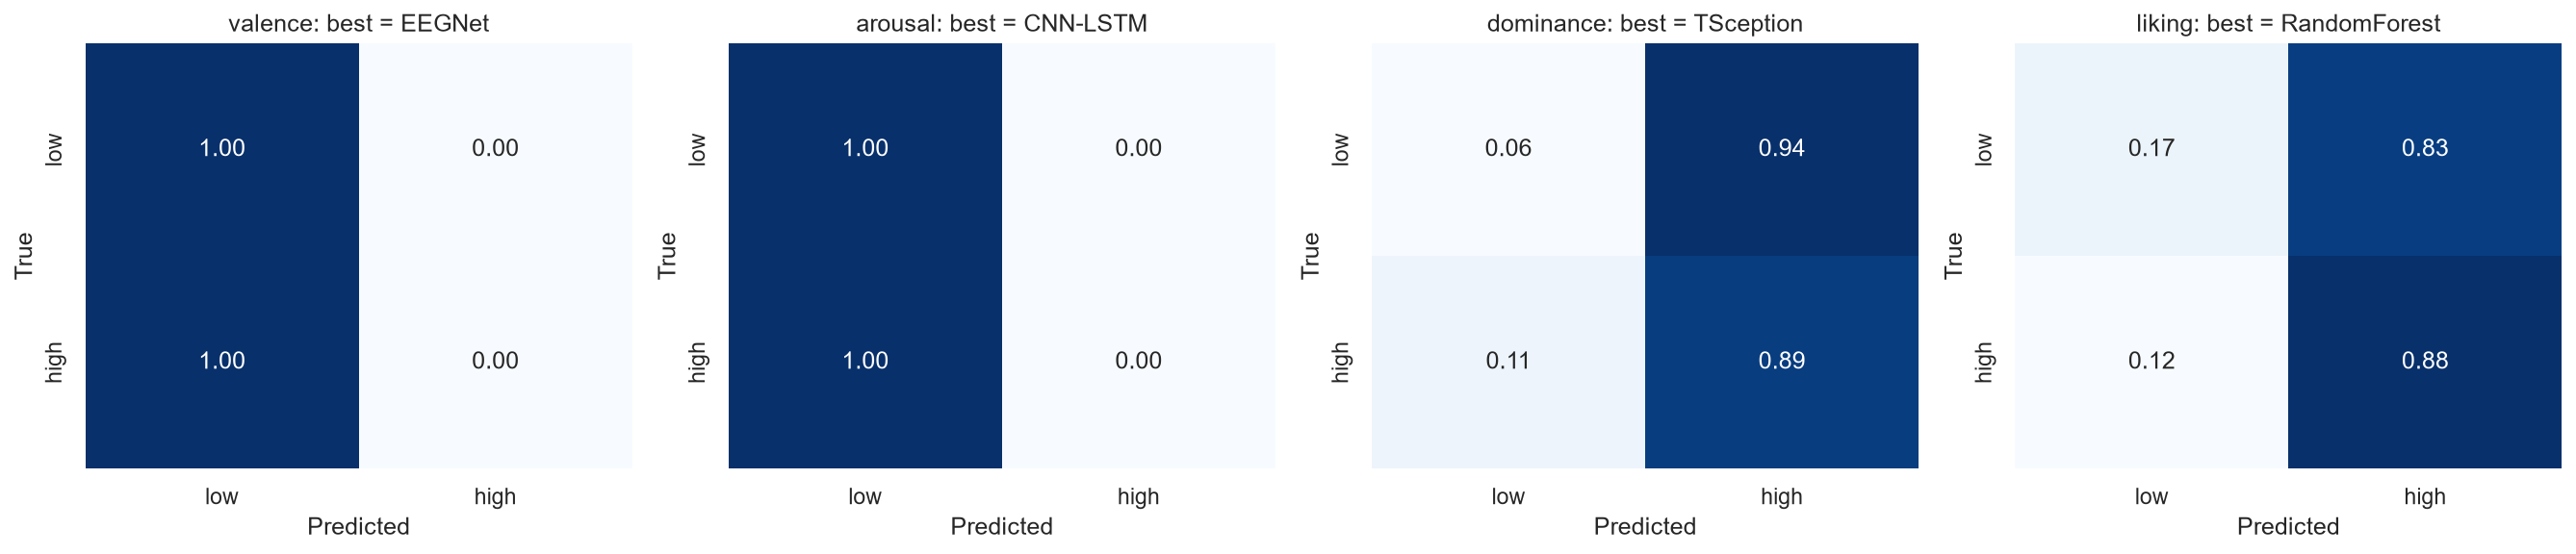
\includegraphics[width=0.85\textwidth]{confusion_matrices_best_models.png}
\caption{Confusion matrices for the highest-\emph{accuracy} model on each
task (EEGNet, CNN-LSTM, TSception, RandomForest). This selection is by mean
accuracy across all 10 models, not by ROC-AUC, which is why the models named
here differ from the AUC-based winners in Tables~\ref{tab:track-a-best} and
\ref{tab:track-b-best}: it is a direct illustration of the accuracy/AUC
divergence under class imbalance discussed in Section~\ref{sec:s8}.}
\label{fig:confusion-matrices}
\end{figure}

\section{Discussion}
\label{sec:s8}
A few points follow directly from the results above:
\begin{itemize}
  \item Neither track wins outright. Track B edges out Track A on valence
        and arousal; Track A edges out Track B on dominance and liking. No
        model on either track clears about 0.61 AUC on any task: every one
        of the 10 models, on every one of the 4 tasks, falls in the
        0.29--0.61 range (dominance/EEGNet the low outlier at 0.288, noted
        above; arousal/EEGNet the high end at 0.607), below chance at the
        bottom and barely above it at the top. This is the first
        appearance of a pattern the rest of this chapter spends many
        sections trying, and mostly failing, to explain away.
  \item The imbalance is not just a caveat, it shows up directly in the
        numbers. Valence is the most skewed task (79\% majority class).
        Track B's valence models hit 83.5\% accuracy at only around 0.56
        AUC: both numbers sit within a couple of points of the 79\% majority
        baseline, the signature of a classifier leaning on class imbalance
        rather than a real signal.
  \item Compute cost differs a lot between tracks. Track A's cheapest models
        (kNN, XGBoost, Logistic Regression) are 10--1000$\times$ cheaper per
        fit than any Track B model, and Track A's numbers are 5-fold
        cross-validated means, while Track B's are single-split point
        estimates (Section~\ref{sec:s11} later adds repeats).
  \item Subject independence is the hard setting. Section~\ref{sec:s13}
        quantifies how much harder: my subject-independent AUC (0.288--0.607
        across all ten models) sits far below the 0.97 ROC-AUC reported on
        the same dataset by \citet{hasan2025methodsx}.
\end{itemize}

\section{Richer Track A features}
\label{sec:s9}
This section tests the most obvious candidate explanation for
Section~\ref{sec:s8}'s near-chance ceiling: that a 128-dimensional
Differential Entropy vector is simply too impoverished a feature set, and a
richer, more diverse description of the same signal would let a classical
model find the signal DE alone misses. I added three additional feature
families to the 128-dim DE baseline (295 features total across 19{,}200
windows), each targeting a different kind of structure DE cannot represent
by construction, since DE only summarises each (channel, band) window's
variance and discards everything else about its shape, timing, and
relationship to other channels:
\begin{itemize}
  \item Hjorth parameters (activity, mobility, complexity)
        \citep{hjorth1970eeg}: 96 features (3 $\times$ 32 channels),
        time-domain complexity descriptors that DE alone misses, since they
        summarise a signal's variance, mean frequency, and frequency spread
        directly from its time-domain derivatives rather than from a
        band-limited variance.
  \item Frontal/hemispheric alpha asymmetry (FAA): 14 features,
        $\text{alpha}_{\text{right}} - \text{alpha}_{\text{left}}$ per
        electrode pair, the classic Davidson-style valence marker
        \citep{davidson1992anterior}, which predicts that positive-valence
        states are associated with relatively greater left-frontal alpha
        suppression (i.e.\ greater left-frontal activation) than
        negative-valence states. It is included specifically because it is
        the one feature family in this report built around a named,
        falsifiable neuroscience hypothesis rather than a generic signal
        descriptor, which lets Section~\ref{sec:s17-5}'s SHAP diagnostic and
        Chapter~\ref{ch:model-analysis}'s TSception analysis test that
        specific hypothesis directly.
  \item Connectivity (PLV and coherence): 57 features across 19 curated
        channel pairs, phase-locking value \citep{lachaux1999plv} in the
        alpha and beta bands (38 features) plus alpha-band
        magnitude-squared coherence (19 features), computed via a
        Hilbert-transform/Welch-style pipeline. Both measures target
        inter-channel synchrony rather than per-channel power, on the
        premise that emotional state may be encoded more in how regions
        communicate than in how much power any single region produces.
\end{itemize}

\subsection{Feature-set ablation}
6 feature-set combinations $\times$ 3 representative models (Logistic
Regression, Random Forest, XGBoost) $\times$ 4 tasks $\times$ 5-fold
\texttt{GroupKFold} gives 360 fits. Mean AUC across all six feature sets
ranges only from 0.478 (DE+Hjorth) to 0.494 (DE+Connectivity): every
individual model/task fit stays in a 0.42--0.56 range, similar to the
classical (non-deep-learning) models in Sections~\ref{sec:s5}--\ref{sec:s6}
but narrower than those sections' full 0.29--0.61 spread once Track B's
deep models are included. None of the three additions move AUC
meaningfully off chance for any task. I carry the ``Full'' set forward to
Section~\ref{sec:s10} as the most complete configuration, not because the
ablation crowned it a clear winner.

\begin{table}[H]
\centering
\caption{Feature-set ablation: mean ROC-AUC across 3 models $\times$ 4
tasks (12 fits) per feature set}
\label{tab:ablation}
\begin{tabular}{lrr}
\toprule
Feature set & \#Features & Mean ROC-AUC \\
\midrule
DE only                       & 128 & 0.479 \\
DE + Hjorth                   & 224 & 0.478 \\
DE + FAA                      & 142 & 0.483 \\
DE + Connectivity             & 185 & 0.494 \\
DE + Hjorth + FAA             & 238 & 0.479 \\
Full (DE+Hjorth+FAA+Conn)     & 295 & 0.483 \\
\bottomrule
\end{tabular}
\end{table}

\begin{figure}[H]
\centering
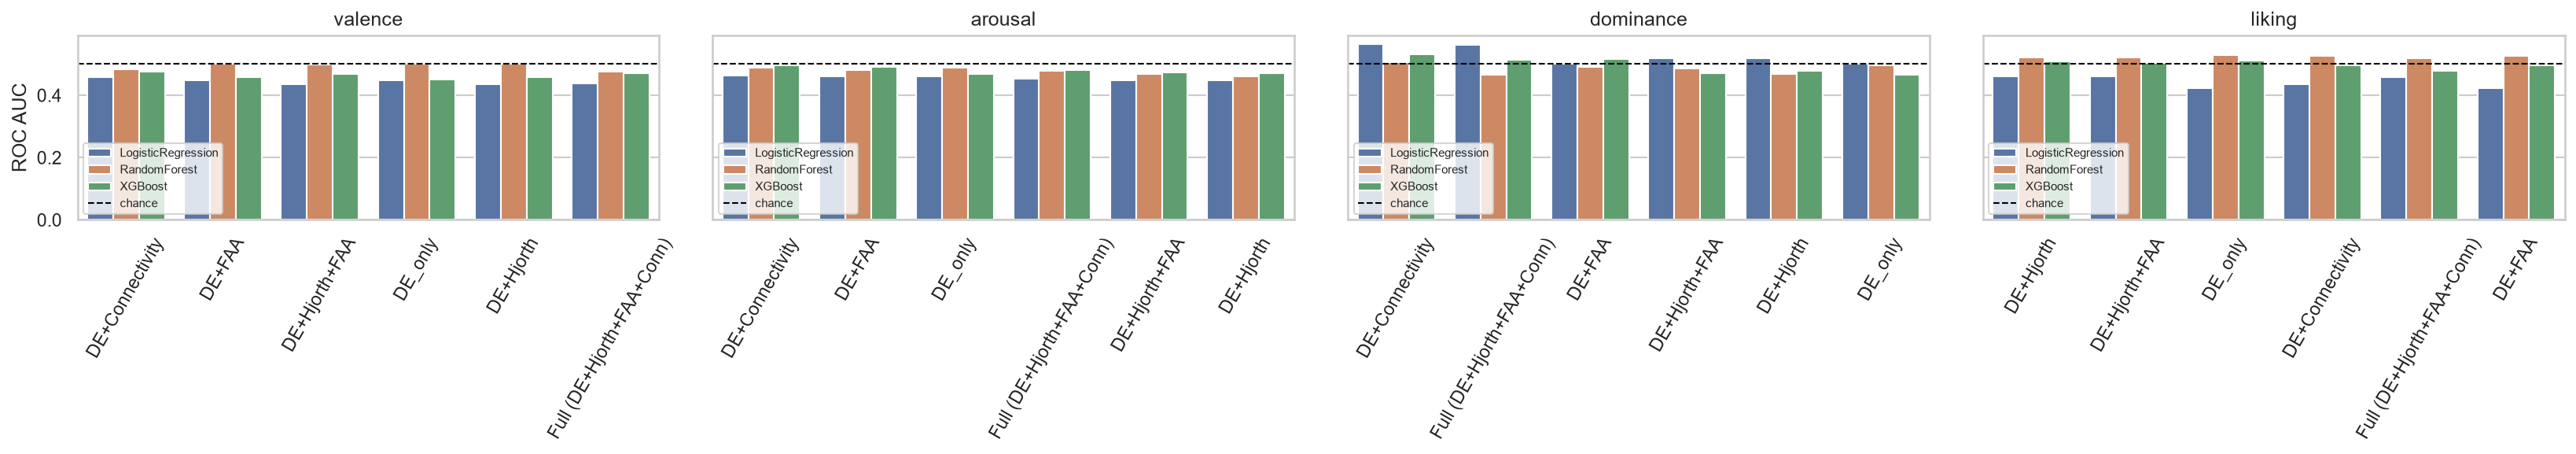
\includegraphics[width=0.85\textwidth]{track_a_ablation_auc.png}
\caption{Feature-set ablation: ROC-AUC by feature set, model, and task.}
\label{fig:ablation}
\end{figure}

\section{Repeated and nested GroupKFold}
\label{sec:s10}
Two upgrades here:
\begin{enumerate}
  \item Repeated GroupKFold (5 repeats $\times$ 5 folds = 25 folds per
        model/task), giving every AUC a real 95\% confidence interval.
        Since \texttt{scikit-learn} has no repeated-group variant, each
        repeat randomly relabels the 32 subject IDs before calling
        \texttt{GroupKFold(5)}, because its greedy fold assignment is
        sensitive to the sorted order of group labels, so relabeling yields
        a different subject-to-fold partition each repeat.
  \item Nested CV for XGBoost and Random Forest: outer \texttt{GroupKFold(5)},
        inner \texttt{GroupKFold(3)} via a randomized hyperparameter search
        (8 draws), to check whether the fixed, hand-picked hyperparameters
        used everywhere else were leaving accuracy on the table.
\end{enumerate}
Of 24 model/task 95\% AUC confidence intervals, 15 contain 0.5 (chance). The
9 that do not skew mostly toward dominance and liking (dominance/Logistic
Regression: 0.571, CI [0.546, 0.597]; liking/kNN: 0.532, CI [0.518, 0.546]).
Nested hyperparameter search does not close the gap either: dominance/XGBoost
reaches 0.494 tuned versus 0.473 with the fixed hyperparameters used
elsewhere in this report (Table~\ref{tab:ma-tracka-auc}), a small +0.021
change that is well within fold-to-fold noise. Table~\ref{tab:nested-cv}
gives the full picture across both tuned models and all four tasks, not just
that one cell: five of the eight tuned/fixed deltas are negative, and the
largest positive delta (dominance/XGBoost, $+0.021$) is barely larger than
the largest negative one (arousal/RandomForest, $-0.035$), so there is no
task on which tuning produces a change that looks different in kind from
fold-to-fold noise. Together, these results rule out fixed hyperparameters
as the main bottleneck.

\begin{table}[H]
\centering
\caption{Nested GroupKFold hyperparameter search: tuned vs.\ fixed-hyperparameter ROC-AUC, RandomForest and XGBoost, all four tasks}
\label{tab:nested-cv}
\begin{tabular}{llrrr}
\toprule
Task & Model & Fixed HP AUC & Tuned AUC & $\Delta$ \\
\midrule
valence   & RandomForest & 0.501 & 0.492 & $-0.009$ \\
valence   & XGBoost      & 0.455 & 0.477 & $+0.022$ \\
arousal   & RandomForest & 0.489 & 0.454 & $-0.035$ \\
arousal   & XGBoost      & 0.483 & 0.470 & $-0.013$ \\
dominance & RandomForest & 0.497 & 0.489 & $-0.008$ \\
dominance & XGBoost      & 0.473 & 0.494 & $+0.021$ \\
liking    & RandomForest & 0.528 & 0.524 & $-0.004$ \\
liking    & XGBoost      & 0.505 & 0.484 & $-0.021$ \\
\bottomrule
\end{tabular}
\end{table}

\begin{figure}[H]
\centering
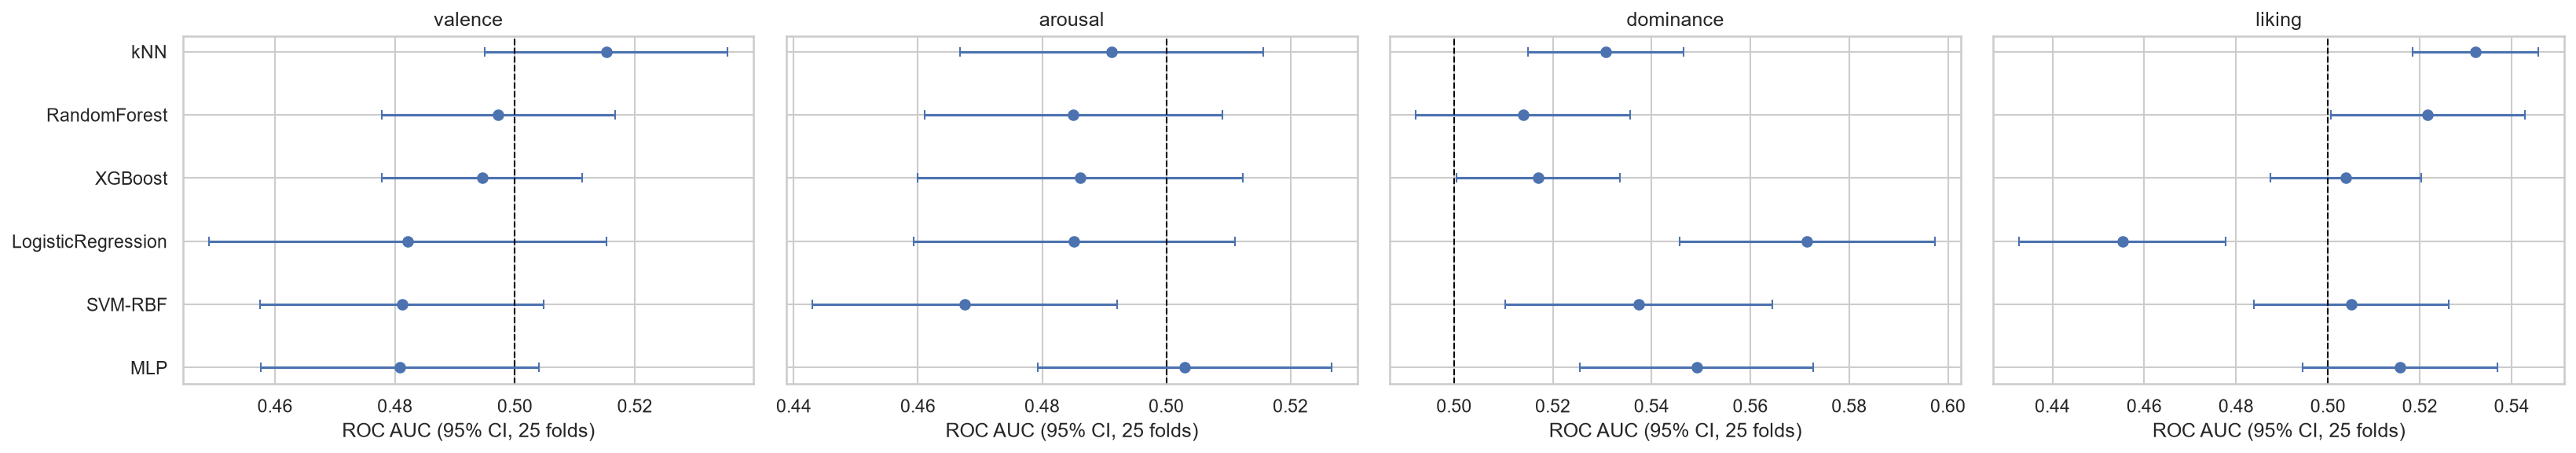
\includegraphics[width=0.9\textwidth]{track_a_repeated_cv_auc_ci.png}
\caption{Repeated GroupKFold (5$\times$5=25 folds): ROC-AUC with 95\%
confidence intervals per model/task; 15/24 intervals contain chance (0.5).}
\label{fig:repeated-cv}
\end{figure}

\section{50\% overlapping windows and repeated Track B splits}
\label{sec:s11}
I built a second raw-window cache with 2\,s stride (50\% overlap) instead of
the original 4\,s stride, giving 29 windows/trial instead of 15
(37{,}120 windows total). This comes with a leakage caveat worth stating up
front: overlapping windows share up to 50\% of their raw samples and are not
independent observations. Subject grouping still prevents cross-subject
leakage, but not this within-subject correlation. I then ran 5 repeated
70/15/15 subject-independent splits, on both window variants, across all 4
architectures and all 4 tasks (160 training runs, about 87 minutes on the
project's RTX 3070 Ti). Mean AUC across all model/task combinations is 0.483
(non-overlap) versus 0.498 (overlap50): the deltas are small and
inconsistent in sign, consistent with the non-independence caveat. More
correlated windows is not the same as more information.

\begin{figure}[H]
\centering
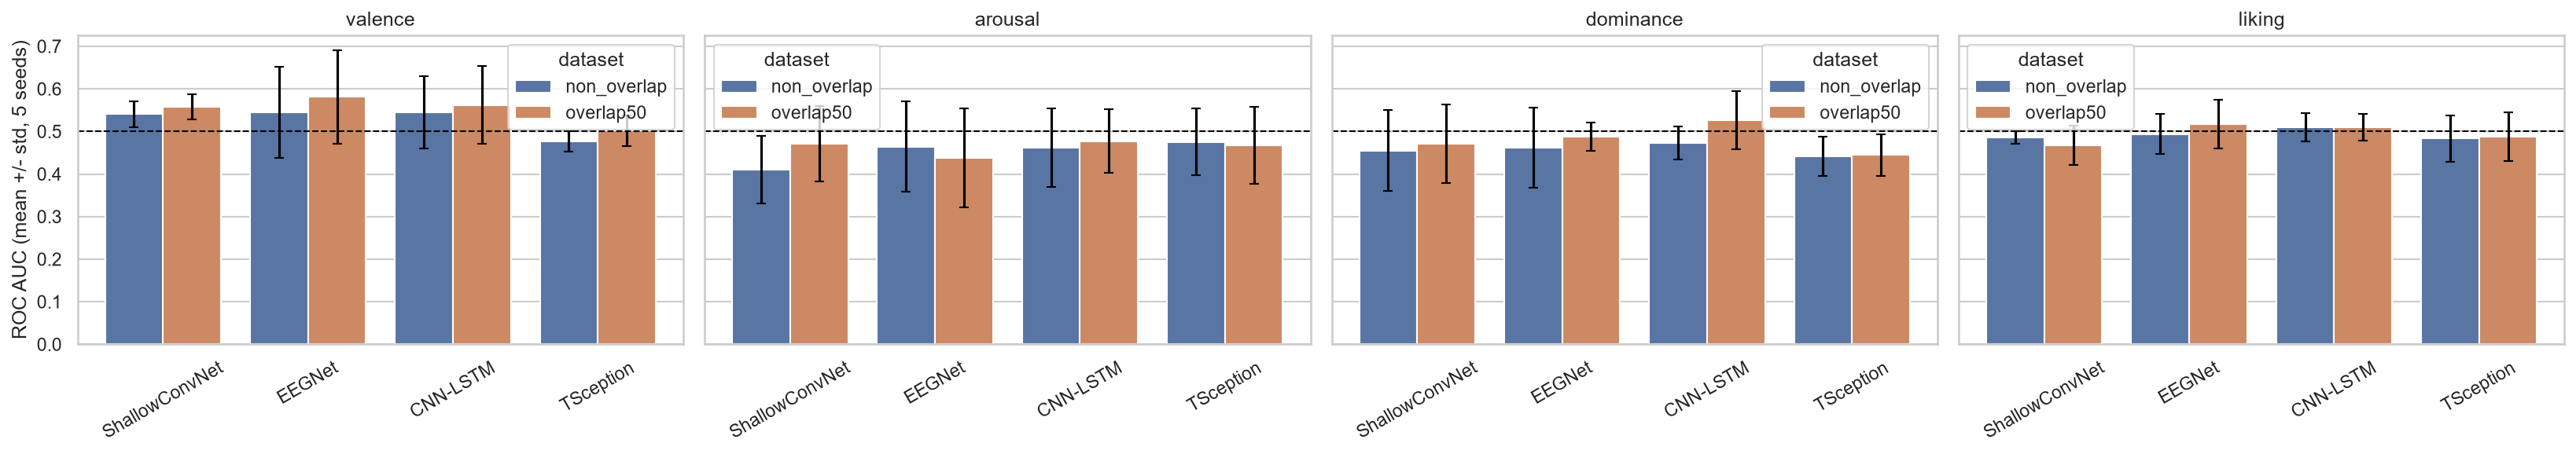
\includegraphics[width=0.85\textwidth]{track_b_overlap_vs_nonoverlap_auc.png}
\caption{Repeated Track B splits: ROC-AUC, non-overlapping vs.\ 50\%-overlap
windows, across 4 architectures $\times$ 4 tasks.}
\label{fig:overlap}
\end{figure}

\section{Cross-corpus validation (SEED-IV)}
\label{sec:s12}
\subsection{Why SEED-IV, not original SEED}
Original SEED requires a signed BCMI data-use agreement; DREAMER and AMIGOS
require similar gated requests. SEED-IV, a related 4-class dataset from the
same lab, is mirrored on Kaggle with no agreement required, so it is the one
target corpus I could actually obtain and run.

\subsection{Pipeline}
\label{sec:seed-iv-adapter}
The cross-corpus code has three parts:
\begin{itemize}
  \item Dataset-agnostic infrastructure: channel-name intersection between
        DEAP and a target montage, polyphase resampling, generic band-DE
        extraction restricted to the common channel subset, rebuilding
        DEAP's own DE features on that same restricted/reordered channel set
        so the DEAP-side model is retrained fairly rather than fed a
        mismatched feature vector, and zero-shot evaluation with a
        per-subject breakdown.
  \item A SEED-IV adapter that loads the 62-channel, 200\,Hz session files,
        resolves the channel-order file defensively across several
        candidate filenames (the Kaggle mirror ships a differently-named and
        differently-capitalised file than originally assumed), and resolves
        per-session labels defensively: it first tries a real label file,
        and, since the download ships no separate label file for this
        purpose, only prose in a README, falls back to the label sequence
        published in the SEED-IV paper. I checked that fallback against the
        README by hand and it matches. SEED-IV's 4 classes are then mapped
        onto a valence-like binary task: happy is positive, sad/fear is
        negative, neutral is dropped.
  \item An orchestration script that runs (1) a within-DEAP
        \texttt{GroupKFold} baseline on the 32 common channels shared with
        SEED-IV, (2) DEAP$\to$SEED-IV zero-shot transfer (train on all of
        DEAP, never see SEED-IV), and (3) a SEED-IV-only LOSO baseline (15
        subjects, 15 folds, one per SEED-IV subject).
\end{itemize}

\subsection{Result}
\begin{table}[h]
\centering
\caption{Cross-corpus validation: DE + XGBoost, 32 common channels}
\label{tab:cross-corpus}
\begin{tabular}{lrrr}
\toprule
Setting & Accuracy & ROC-AUC & Notes \\
\midrule
Within-DEAP GroupKFold      & 0.756 & 0.452 & below chance point estimate \\
DEAP$\to$SEED-IV zero-shot  & 0.709 & 0.517 & marginally above chance \\
SEED-IV-only LOSO           & 0.709 & 0.673 & 14/15 subjects $>$0.55 AUC \\
\bottomrule
\end{tabular}
\end{table}

Table~\ref{tab:cross-corpus-per-subject} gives the full per-subject breakdown
behind the SEED-IV-only LOSO row above: 14 of the 15 held-out subjects clear
0.55 AUC; the single exception is subject 97132107 at 0.515, still close to
chance but not below it. There is no subject whose result is so far below
chance that it would be worth excluding as an anomaly; the spread
(0.515--0.880) is wide but one-sided, consistent with the pipeline finding a
real, if uneven, signal on this corpus rather than noise centred on 0.5.

\begin{table}[H]
\centering
\caption{SEED-IV-only Leave-One-Subject-Out: per-subject ROC-AUC (DE + XGBoost, 32 common channels)}
\label{tab:cross-corpus-per-subject}
\begin{tabular}{lrrr}
\toprule
Held-out subject & Accuracy & F1 (macro) & ROC-AUC \\
\midrule
10230076 & 0.833 & 0.795 & 0.880 \\
17741077 & 0.808 & 0.737 & 0.796 \\
84163914 & 0.734 & 0.539 & 0.744 \\
43091099 & 0.742 & 0.682 & 0.759 \\
23084164 & 0.784 & 0.648 & 0.720 \\
48942731 & 0.737 & 0.626 & 0.707 \\
59416627 & 0.716 & 0.649 & 0.673 \\
35646451 & 0.717 & 0.565 & 0.670 \\
99723240 & 0.675 & 0.563 & 0.663 \\
61771259 & 0.710 & 0.438 & 0.609 \\
82638880 & 0.645 & 0.574 & 0.621 \\
43051602 & 0.714 & 0.462 & 0.595 \\
75903953 & 0.452 & 0.452 & 0.560 \\
59481326 & 0.656 & 0.547 & 0.582 \\
97132107 & 0.709 & 0.441 & 0.515 \\
\bottomrule
\end{tabular}
\end{table}
This changes how I read the question this section set out to answer. DEAP's
own within-corpus signal is not inflated relative to cross-corpus transfer;
it is the weakest of the three settings here. The identical pipeline reaches
a moderate AUC of 0.673 on SEED-IV under a directly comparable protocol.
That is one 3-setting comparison with a single model on a dataset with a
different label construct (a 4-class emotion label collapsed to a
happy-vs-sad/fear binary task, rather than DEAP's continuous valence
threshold), so it supports the more modest claim that the near-chance
ceiling may be specific to DEAP, rather than ruling out a general
explanation for weak subject-independent EEG emotion decoding. Other
caveats: the two corpora differ in session count and per-trial duration, and
restricting to 32 common channels discards SEED-IV's denser 62-channel
coverage.

\begin{figure}[H]
\centering
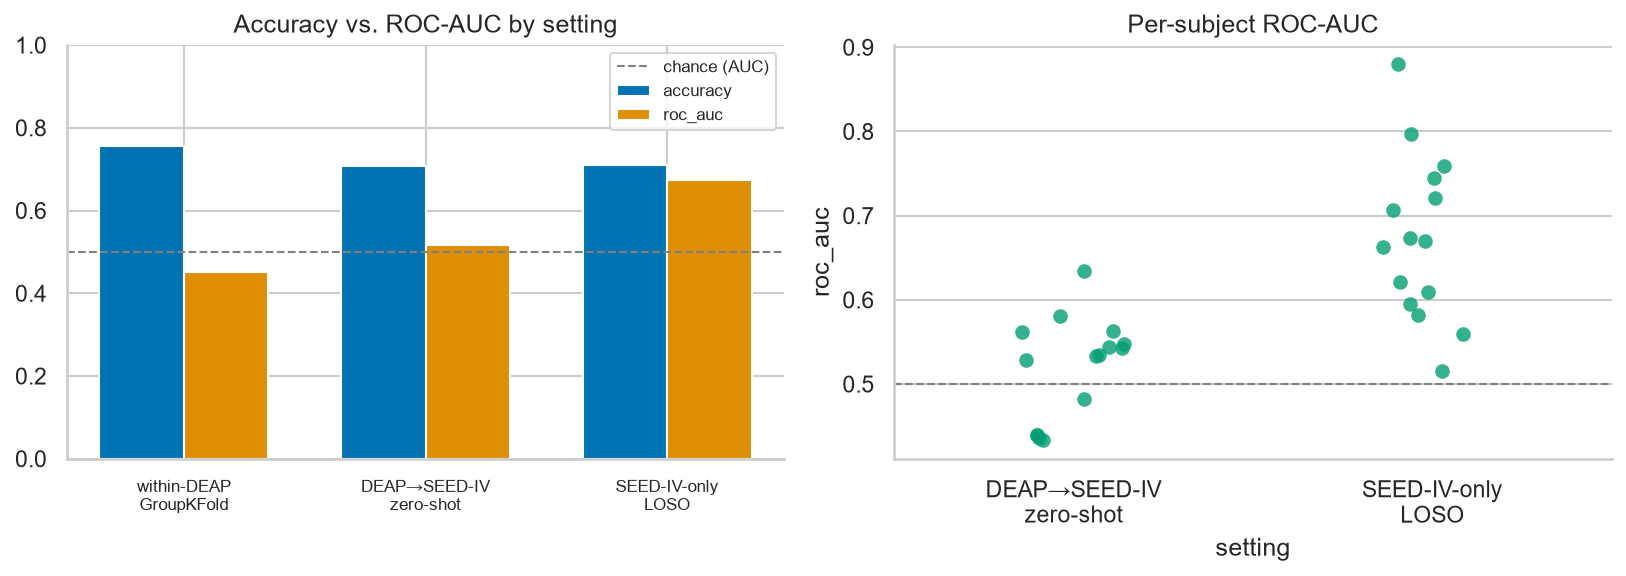
\includegraphics[width=0.85\textwidth]{cross_corpus_deap_seediv.png}
\caption{Cross-corpus validation: ROC-AUC across the three settings of
Table~\ref{tab:cross-corpus} (within-DEAP, DEAP$\to$SEED-IV zero-shot,
SEED-IV-only LOSO).}
\label{fig:cross-corpus}
\end{figure}

\section{Extended discussion}
\label{sec:s13}
Pulling together Sections~\ref{sec:s9}--\ref{sec:s12}: AUC hovers within
noise of chance almost everywhere, and this is the single most important
finding in this report. None of richer features, repeated/nested CV, or
window overlap fixed the ceiling, which is itself informative: each rules
out a specific, plausible cause rather than pointing to a failed
implementation. The cross-corpus result overturns my own original guess that
a weak DEAP signal would mean weak transfer too, and instead suggests the
ceiling may be specific to DEAP rather than universal (Section~\ref{sec:s12}).
The practical recommendation I would make for any paper drawn from this work
is to lead with the leaky-split contrast: my own 0.288--0.607 AUC under
leakage-free \texttt{GroupKFold}, versus the 0.97 ROC-AUC reported on the same
dataset and a similar feature/classifier combination by
\citet{hasan2025methodsx}.

\section{Label-cleanup ablation}
\label{sec:s14}
I tested three ways of turning continuous ratings into binary labels (Full
feature set, 3 models, 4 tasks, \texttt{GroupKFold(5)}):
\begin{itemize}
  \item raw threshold (baseline): fixed cutoff at 5.0.
  \item per-subject z-score: z-score each subject's own 40 ratings before
        thresholding at 0, correcting for individual anchoring bias.
  \item drop-middle: keep only ratings $\le3$ or $\ge6$, discarding the
        ambiguous middle.
\end{itemize}
Mean AUC is 0.483 (raw threshold), 0.514 (per-subject z-score), 0.487
(drop-middle). Per-subject z-scoring rebalances classes substantially
(valence goes from 21.0\% to 47.3\% high) and gives the largest AUC bump,
but the gain is modest, and the class-balance shift means its accuracy
numbers should not be compared directly to the baseline's. Neither
alternative beats the baseline by enough to conclude that the fixed
threshold was the main bottleneck.

\begin{table}[H]
\centering
\caption{Label-cleanup ablation: mean ROC-AUC across 3 models $\times$
4 tasks per label variant}
\label{tab:label-cleanup}
\begin{tabular}{lr}
\toprule
Label variant & Mean ROC-AUC \\
\midrule
raw\_threshold (baseline) & 0.483 \\
per\_subject\_z           & 0.514 \\
drop\_middle               & 0.487 \\
\bottomrule
\end{tabular}
\end{table}

\begin{figure}[H]
\centering
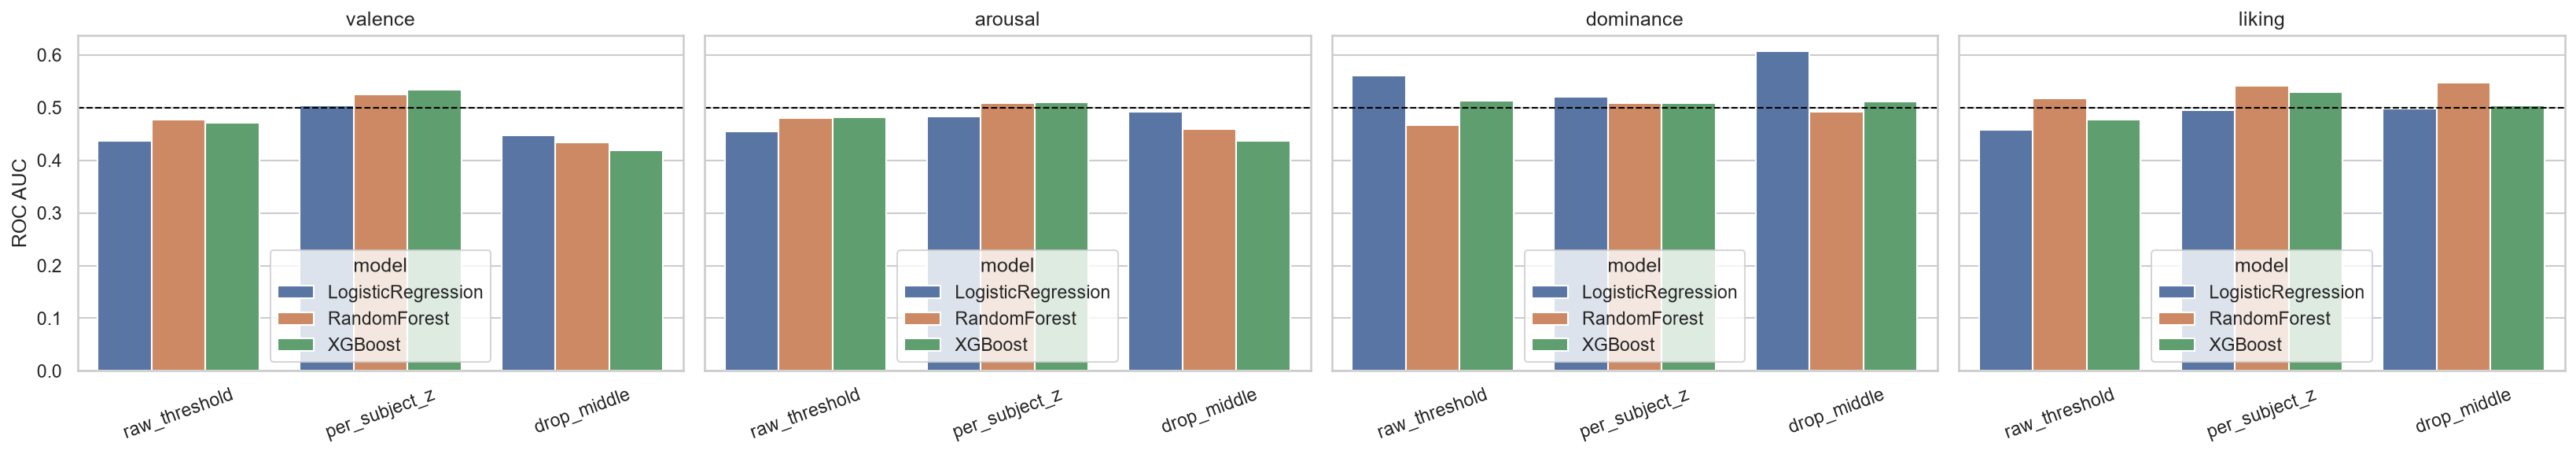
\includegraphics[width=0.85\textwidth]{track_a_label_cleanup_auc.png}
\caption{Label-cleanup ablation: ROC-AUC by label variant, model, and
task.}
\label{fig:label-cleanup}
\end{figure}

\section{Per-subject calibration (personalisation)}
\label{sec:s15}
I ran a true 32-fold Leave-One-Subject-Out with XGBoost, which is cheap
enough to make full LOSO tractable (about 13\,s/subject). For each held-out
subject: train a base model on the other 31 subjects; split the held-out
subject's 40 trials 80/20 into eval/calibration sets, by trial, so a
trial's 15 windows never cross the split; score the base model zero-shot on
the eval set; then warm-start about 40 extra boosted trees on the 8-trial
calibration set only, and re-score on the identical eval set. Subjects whose
calibration set is single-class (13 across all 4 tasks) are skipped for the
calibrated arm and reported as such. Mean zero-shot AUC is around 0.50--0.51
across all four tasks; mean calibrated AUC rises to 0.577 (arousal), 0.519
(dominance), 0.539 (liking), 0.537 (valence), a modest positive shift from a
small amount of the target subject's own data. This suggests the ceiling is
not purely a between-subject-variability problem that a little calibration
data cannot touch, though 8 trials and 40 trees is a small intervention.

\begin{figure}[H]
\centering
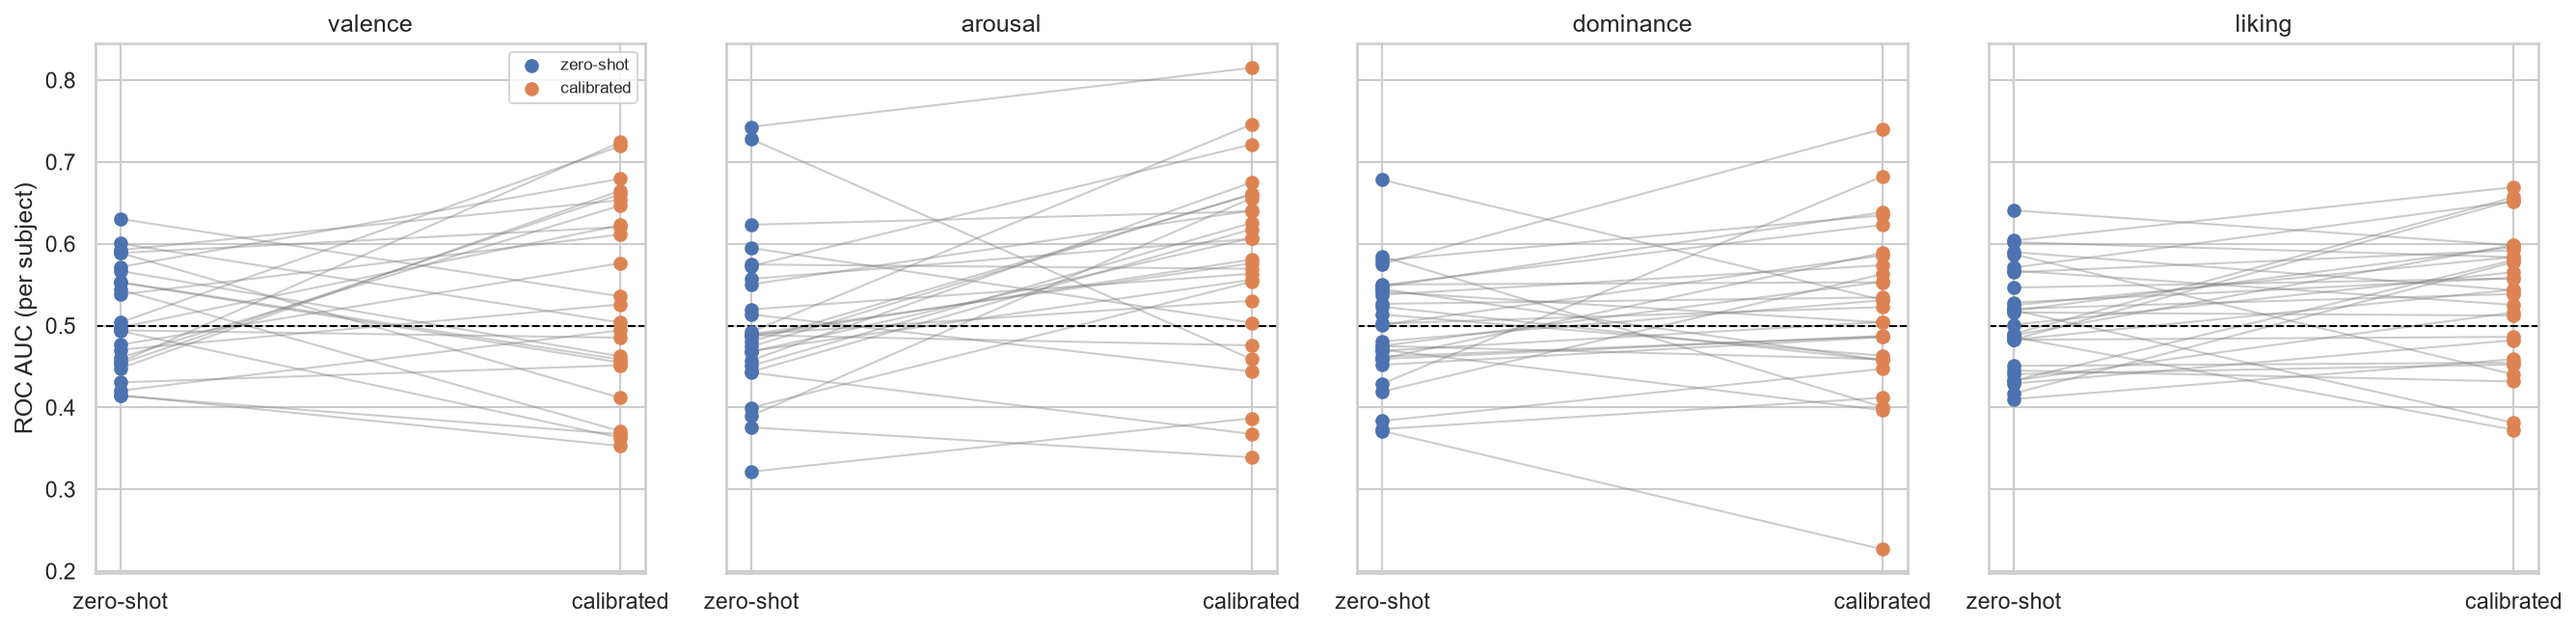
\includegraphics[width=0.9\textwidth]{track_a_calibration_per_subject.png}
\caption{Per-subject LOSO calibration: zero-shot vs.\ calibrated ROC-AUC
for each of the 32 held-out subjects, per task.}
\label{fig:calibration}
\end{figure}

\section{Literature-driven interventions}
\label{sec:s16}
32 papers in \texttt{papers\_EEG/} were assembled and reviewed (see
Chapter~\ref{ch:literature}), yielding three untried interventions.

\subsection{Permutation significance test}
\label{sec:s16-1}
I shuffle labels at the trial level within each subject (each subject keeps
its own true set of 40 trial labels; only which of that subject's trials
gets which label is permuted), then propagate each shuffled trial label to
all 15 windows of that trial, rerun the exact Full-feature-set
\texttt{GroupKFold(5)} pipeline with Logistic Regression as a fast proxy, and
repeat this 300 times per task to build an empirical null AUC distribution;
$p = \frac{1 + \#\{\text{null} \ge \text{observed}\}}{n_{\text{perm}}+1}$.
Permuting at the trial level rather than the window level matters: an
earlier version of this test shuffled all 19{,}200 window-level labels
independently, which treats a trial's 15 windows as exchangeable when they
in fact share one label. That inflated the null's effective sample size and
collapsed its spread (std $\approx0.005$), which in turn inflated every
z-score, including dominance's. Once permutation respects the trial/subject
structure, the null is roughly five times wider (std
$\approx0.022$--$0.028$), and its mean is free to drift away from 0.5 per
task (e.g.\ arousal's null mean is $0.532$) since each permutation still
preserves each subject's real, imbalanced trial counts. Under this corrected
test, valence, arousal, and liking's observed AUC is no longer
distinguishable from the null ($z=-2.25$, $-2.90$, $-1.12$; $p=0.993$,
$0.997$, $0.877$), so the earlier claim that they sit significantly
\emph{below} chance does not survive the correction. Dominance remains the
only task whose observed AUC clears the null (observed 0.561 vs.\ null
$0.499\pm0.028$, $z=+2.18$, $p=0.0199$), but the effect has shrunk sharply
from the buggy version ($p=0.0033\to p=0.0199$) and does not survive a
Bonferroni correction for testing four tasks ($\alpha=0.05/4=0.0125$). The
honest reading of the corrected test is that no task's AUC is robustly
distinguishable from a properly-built, trial-respecting chance baseline.

\begin{table}[H]
\centering
\caption{Permutation significance test (300 shuffles per task, trial-within-subject permutation, LogisticRegression proxy)}
\label{tab:significance}
\begin{tabular}{lrrrr}
\toprule
Task & Observed AUC & Null mean $\pm$ std & $z$ & $p$ \\
\midrule
valence   & 0.437 & $0.495\pm0.026$ & $-2.25$ & 0.9934 \\
arousal   & 0.454 & $0.532\pm0.027$ & $-2.90$ & 0.9967 \\
dominance & 0.561 & $0.499\pm0.028$ & $+2.18$ & 0.0199 \\
liking    & 0.458 & $0.482\pm0.022$ & $-1.12$ & 0.8771 \\
\bottomrule
\end{tabular}
\end{table}

\begin{figure}[H]
\centering
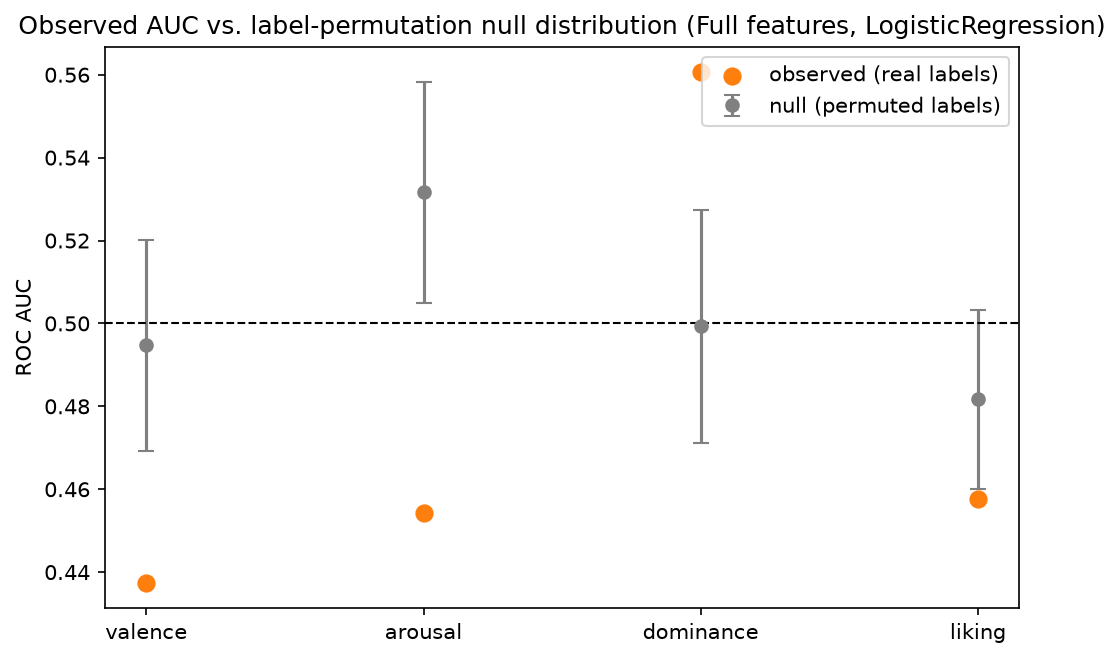
\includegraphics[width=0.85\textwidth]{track_a_significance_test.png}
\caption{Permutation null AUC distributions vs.\ observed AUC, per task.}
\label{fig:significance}
\end{figure}

\subsection{CORAL feature alignment}
\label{sec:s16-2}
I implemented CORAL \citep{sun2016coral}: per \texttt{GroupKFold} fold,
whiten the training fold's features by their own covariance and recolour by
the unlabelled test fold's covariance, via eigendecomposition-based matrix
square roots with a ridge for numerical stability. Mean AUC delta across 12
task/model combinations is $+0.0059$ (8/12 improved, 4/12 worse), small and
inconsistent in sign.

\begin{table}[H]
\centering
\caption{CORAL alignment: mean ROC-AUC across 3 models per task}
\label{tab:coral}
\begin{tabular}{lrrr}
\toprule
Task & No alignment & CORAL & $\Delta$ \\
\midrule
valence   & 0.462 & 0.478 & $+0.016$ \\
arousal   & 0.472 & 0.476 & $+0.004$ \\
dominance & 0.514 & 0.521 & $+0.008$ \\
liking    & 0.484 & 0.480 & $-0.004$ \\
\bottomrule
\end{tabular}
\end{table}

\begin{figure}[H]
\centering
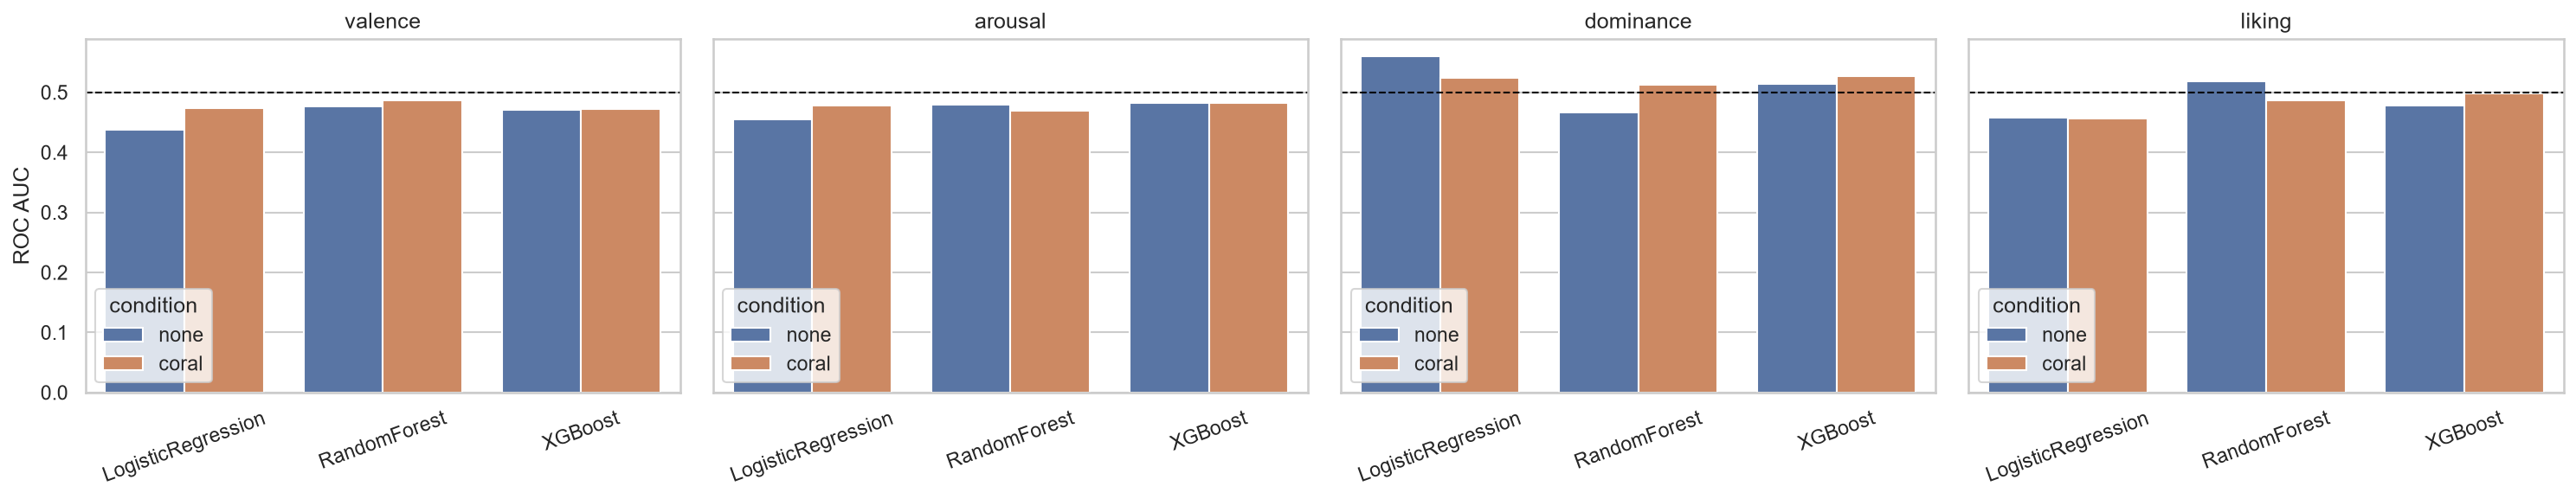
\includegraphics[width=0.85\textwidth]{track_a_domain_alignment_auc.png}
\caption{CORAL alignment: ROC-AUC before/after, by model and task.}
\label{fig:coral}
\end{figure}

\subsection{Subject-adversarial (DANN) training}
\label{sec:s16-3}
\emph{A note on the EEGNet baseline used from here on}: Table~\ref{tab:track-b-best}
reports EEGNet's valence AUC as 0.561, from the main notebook's single
70/15/15 split. Sections~\ref{sec:s16-3} through \ref{sec:s17} instead use
0.474 as the EEGNet valence ``no intervention'' baseline. Both numbers are
correct for what they measure: they come from separate script runs with a
different train/val/test split and seed than the main notebook cell, since
each companion script draws its own split rather than reusing the
notebook's. I have not reconciled the two into a single number; they should
be read as two separate point estimates of the same quantity rather than a
single ground truth.

I added a gradient-reversal-layer (GRL) domain classifier to EEGNet, trained
to predict the training-fold subject's identity; the GRL reverses that
gradient before it reaches the shared encoder, using the standard
\citet{ganin2015dann} progressive-$\lambda$ schedule. The outcome is mixed and
task-dependent. Valence AUC $0.474\to0.513$ ($+0.039$) and liking AUC
$0.467\to0.517$ ($+0.050$) improved; arousal AUC $0.616\to0.400$ ($-0.216$)
and dominance AUC $0.552\to0.403$ ($-0.149$) collapsed, with precision and
recall pinned near 0.50, the classifier collapsing toward one class rather
than a milder generic drop. This matches a documented failure pattern in
unsupervised domain adaptation, over-aggressive alignment collapsing class
structure, described in one of the survey papers in the literature corpus
\citep{sreehari2026review}.

\begin{table}[H]
\centering
\caption{Subject-adversarial (DANN) training: ROC-AUC, EEGNet, single split}
\label{tab:dann}
\begin{tabular}{lrrr}
\toprule
Task & Baseline & DANN & $\Delta$ \\
\midrule
valence   & 0.474 & 0.513 & $+0.039$ \\
arousal   & 0.616 & 0.400 & $-0.216$ \\
dominance & 0.552 & 0.403 & $-0.149$ \\
liking    & 0.467 & 0.517 & $+0.050$ \\
\bottomrule
\end{tabular}
\end{table}

\begin{figure}[H]
\centering
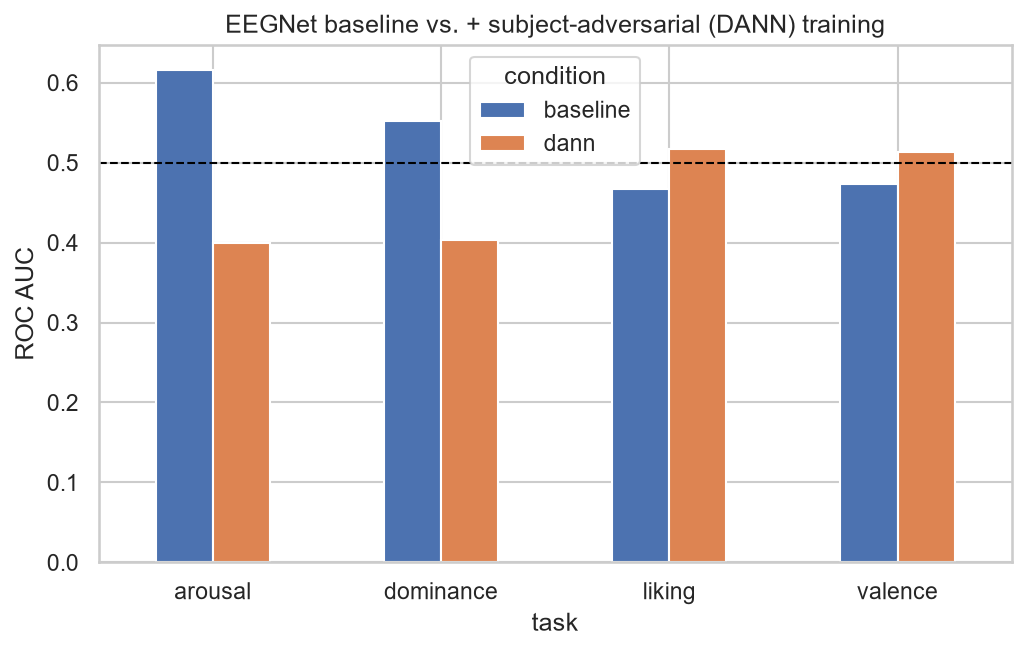
\includegraphics[width=0.85\textwidth]{track_b_domain_adversarial_auc.png}
\caption{DANN training: ROC-AUC before/after, per task; note the
arousal/dominance collapse.}
\label{fig:dann}
\end{figure}

\section{Five deferred literature techniques}
\label{sec:s17}

\subsection{Euclidean Alignment}
\label{sec:s17-1}
I implemented Euclidean Alignment, EA \citep{he2019euclidean}: per subject, compute
each window's raw spatial covariance $C_i = X_i X_i^\top / T$, average
across that subject's windows to get $\bar R$, then whiten every window by
$\bar R^{-1/2}$ before DE features are recomputed. This is an upstream,
per-subject, label-free, raw-channel-level transform, unlike CORAL's
downstream per-fold feature-level operation. This is the strongest effect I
found in the whole project: mean AUC delta $+0.044$ across 12 task/model
combinations (10/12 improved), and unlike every other alignment technique I
tried, the sign is consistent within three of the four tasks (valence
+0.087/+0.027/+0.069, arousal +0.078/+0.027/+0.065, dominance
+0.074/+0.038/+0.073 across LR/RF/XGBoost). It is still modest in absolute
terms: the best post-EA AUCs land around 0.53--0.58.

\begin{table}[H]
\centering
\caption{Euclidean Alignment: mean ROC-AUC across 3 models per task}
\label{tab:ea}
\begin{tabular}{lrrr}
\toprule
Task & No alignment & EA & $\Delta$ \\
\midrule
valence   & 0.467 & 0.528 & $+0.061$ \\
arousal   & 0.473 & 0.530 & $+0.057$ \\
dominance & 0.488 & 0.550 & $+0.062$ \\
liking    & 0.488 & 0.485 & $-0.003$ \\
\bottomrule
\end{tabular}
\end{table}

\begin{figure}[H]
\centering
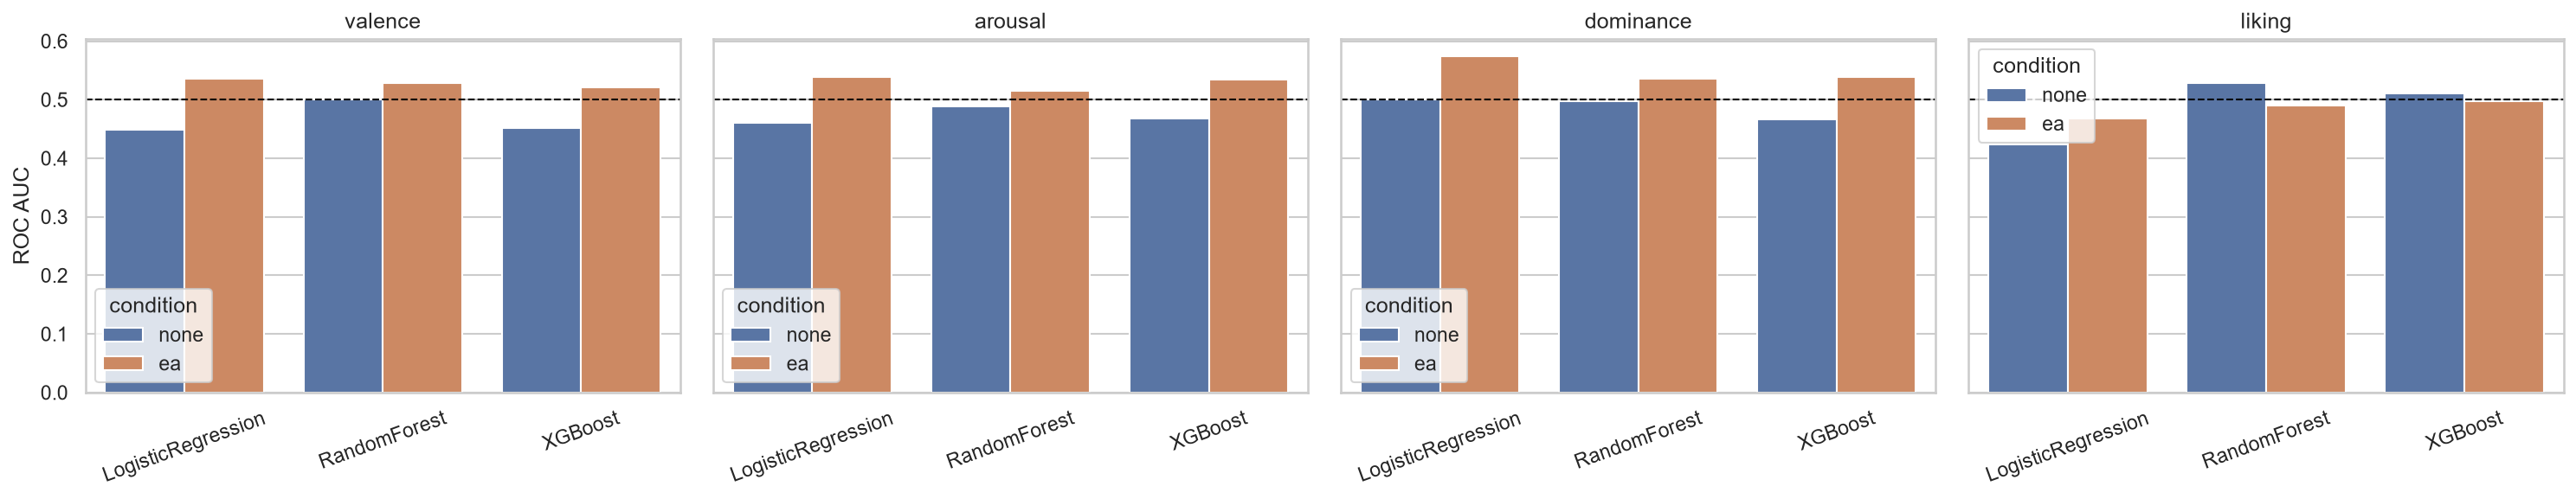
\includegraphics[width=0.85\textwidth]{track_a_riemannian_alignment_auc.png}
\caption{Euclidean Alignment: ROC-AUC before/after, by model and task,
the strongest effect found in the project.}
\label{fig:ea}
\end{figure}

\subsection{Self-supervised (TFR-style) pretraining}
\label{sec:s17-2}
I pretrained EEGNet's conv trunk with a label-free MSE regression pretext
task, predicting each window's own 32-channel $\times$ 4-band log-band-power
from the raw signal using training-fold subjects only, then fine-tuned end
to end and compared against an identically trained scratch EEGNet. The
result is a bimodal, task-split pattern: valence AUC $0.474\to0.547$
($+0.074$) and liking $0.467\to0.567$ ($+0.100$) improved, while arousal
$0.616\to0.534$ ($-0.082$) and dominance $0.552\to0.500$ ($-0.053$) got
worse. The pretext task itself converged fine, with MSE dropping over 15
epochs, so this is not a training-failure artifact.

\begin{table}[H]
\centering
\caption{SSL pretraining: ROC-AUC, EEGNet, single split}
\label{tab:ssl}
\begin{tabular}{lrrr}
\toprule
Task & Scratch & SSL-pretrained & $\Delta$ \\
\midrule
valence   & 0.474 & 0.547 & $+0.074$ \\
arousal   & 0.616 & 0.534 & $-0.082$ \\
dominance & 0.552 & 0.500 & $-0.053$ \\
liking    & 0.467 & 0.567 & $+0.100$ \\
\bottomrule
\end{tabular}
\end{table}

\begin{figure}[H]
\centering
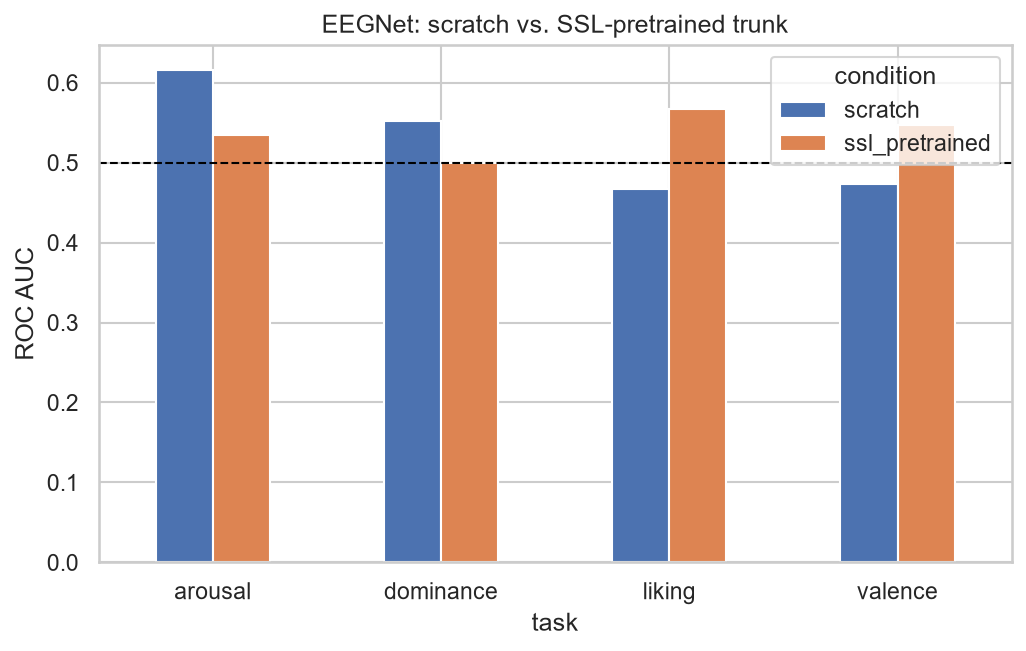
\includegraphics[width=0.85\textwidth]{track_b_ssl_pretrain_auc.png}
\caption{SSL pretraining: ROC-AUC, scratch vs.\ pretrained, per task.}
\label{fig:ssl}
\end{figure}

\subsection{AUC-margin training loss}
\label{sec:s17-3}
I replaced cross-entropy with a mini-batch pairwise squared-hinge AUC
surrogate, $L = \text{mean}_{i \in \text{pos}, j \in \text{neg}} \max(0, m -
(s_i - s_j))^2$, a simplified, self-contained version of the Xiao (2024)
AUC-maximization objective, not the source paper's full saddle-point solver.
This is the one intervention with a clear mechanism behind it. Valence
improved most (AUC $0.474\to0.557$, $+0.083$): the cross-entropy baseline's
83.5\% accuracy at 0.474 AUC was a majority-class collapse, and the
AUC-margin loss produced a more balanced classifier (accuracy 0.507, AUC
0.557) because it is insensitive to that imbalance by construction.
Dominance improved slightly ($+0.008$); arousal ($-0.010$) and liking
($-0.018$) were small changes, likely within noise.

\begin{table}[H]
\centering
\caption{AUC-margin loss: ROC-AUC, EEGNet, single split}
\label{tab:aucmax}
\begin{tabular}{lrrr}
\toprule
Task & CE baseline & AUC-margin & $\Delta$ \\
\midrule
valence   & 0.474 & 0.557 & $+0.083$ \\
arousal   & 0.616 & 0.606 & $-0.010$ \\
dominance & 0.552 & 0.560 & $+0.008$ \\
liking    & 0.467 & 0.450 & $-0.018$ \\
\bottomrule
\end{tabular}
\end{table}

\begin{figure}[H]
\centering
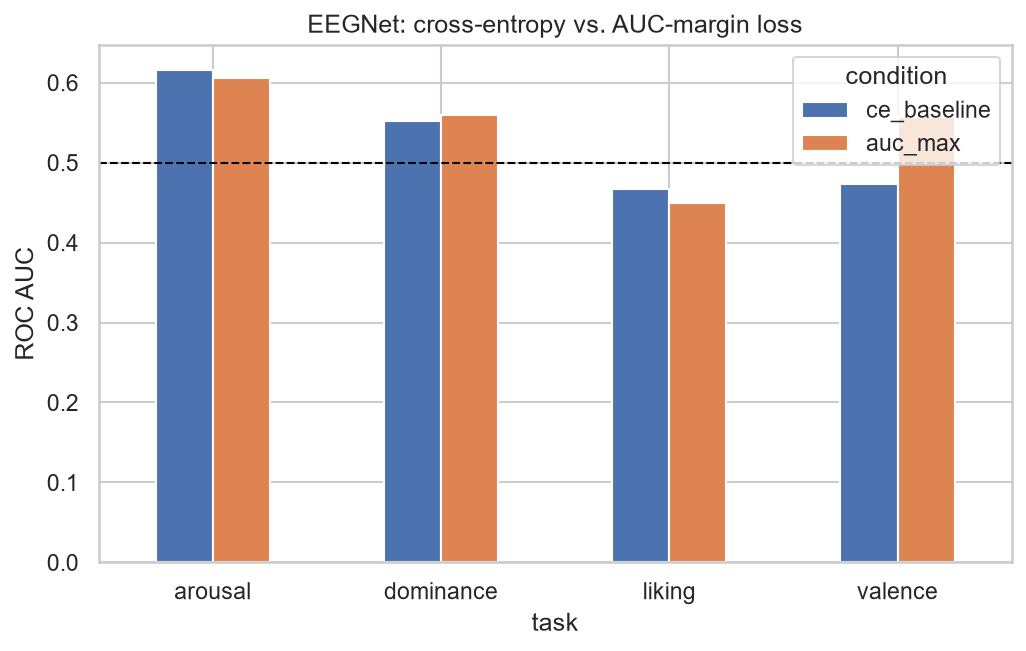
\includegraphics[width=0.85\textwidth]{track_b_auc_maximization_auc.png}
\caption{AUC-margin loss: ROC-AUC, cross-entropy vs.\ AUC-margin, per
task.}
\label{fig:aucmax}
\end{figure}

\subsection{AdaBN test-time adaptation}
\label{sec:s17-4}
I recomputed every BatchNorm layer's running statistics using only a
held-out test subject's own unlabelled windows, with no gradients and no
labels, then evaluated with the adapted statistics. The net effect is
negative overall. Arousal AUC $0.616\to0.515$ ($-0.101$) and dominance
$0.552\to0.489$ ($-0.063$) got worse; liking $0.467\to0.549$ ($+0.082$)
improved; valence was flat ($+0.002$). This is the only clearly net-negative
intervention in Section~\ref{sec:s17}.

\begin{table}[H]
\centering
\caption{AdaBN test-time adaptation: ROC-AUC, EEGNet, single split}
\label{tab:adabn}
\begin{tabular}{lrrr}
\toprule
Task & No adaptation & AdaBN & $\Delta$ \\
\midrule
valence   & 0.474 & 0.476 & $+0.002$ \\
arousal   & 0.616 & 0.515 & $-0.101$ \\
dominance & 0.552 & 0.489 & $-0.063$ \\
liking    & 0.467 & 0.549 & $+0.082$ \\
\bottomrule
\end{tabular}
\end{table}

\begin{figure}[H]
\centering
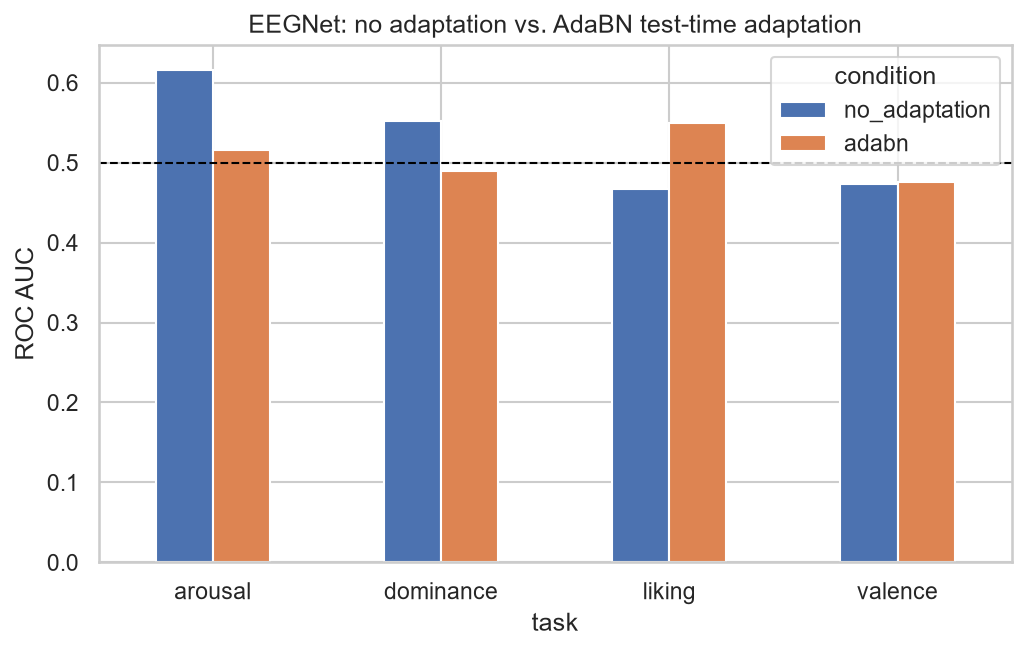
\includegraphics[width=0.85\textwidth]{track_b_test_time_adaptation_auc.png}
\caption{AdaBN test-time adaptation: ROC-AUC before/after, per task.}
\label{fig:adabn}
\end{figure}

\subsection{SHAP interpretability diagnostic}
\label{sec:s17-5}
I fit XGBoost on the Full feature set, one representative fold per task, and
computed SHAP values on the held-out fold, aggregated by feature family and
individually. Importance is spread across families roughly in proportion to
how many features each contributes, with two mild departures: DE's share
(47--52\%) and Connectivity's (22--24\%) both sit slightly above their
feature-count share, while Hjorth's (21--26\%) sits below. Frontal/hemispheric
alpha asymmetry, the one feature family built around a named
neurophysiological hypothesis, carries the smallest importance share in
every task (3.4--6.1\%). The top individual features are diffuse spectral
and connectivity structure (\texttt{de\_beta\_P4} for valence,
\texttt{de\_gamma\_FC2} for arousal and liking, \texttt{plv\_beta\_F3-O1} for
dominance), not FAA. Table~\ref{tab:shap-family-share} gives the exact
per-task percentages behind those ranges.

\begin{table}[H]
\centering
\caption{SHAP diagnostic: mean absolute SHAP importance share (\%) by feature family and task}
\label{tab:shap-family-share}
\begin{tabular}{lrrrr}
\toprule
Task & DE & Hjorth & FAA & Connectivity \\
\midrule
valence   & 50.7 & 21.5 & 3.7 & 24.2 \\
arousal   & 51.8 & 23.0 & 3.4 & 21.8 \\
dominance & 47.2 & 22.9 & 6.1 & 23.8 \\
liking    & 46.8 & 25.7 & 4.4 & 23.1 \\
\bottomrule
\end{tabular}
\end{table}

\begin{figure}[H]
\centering
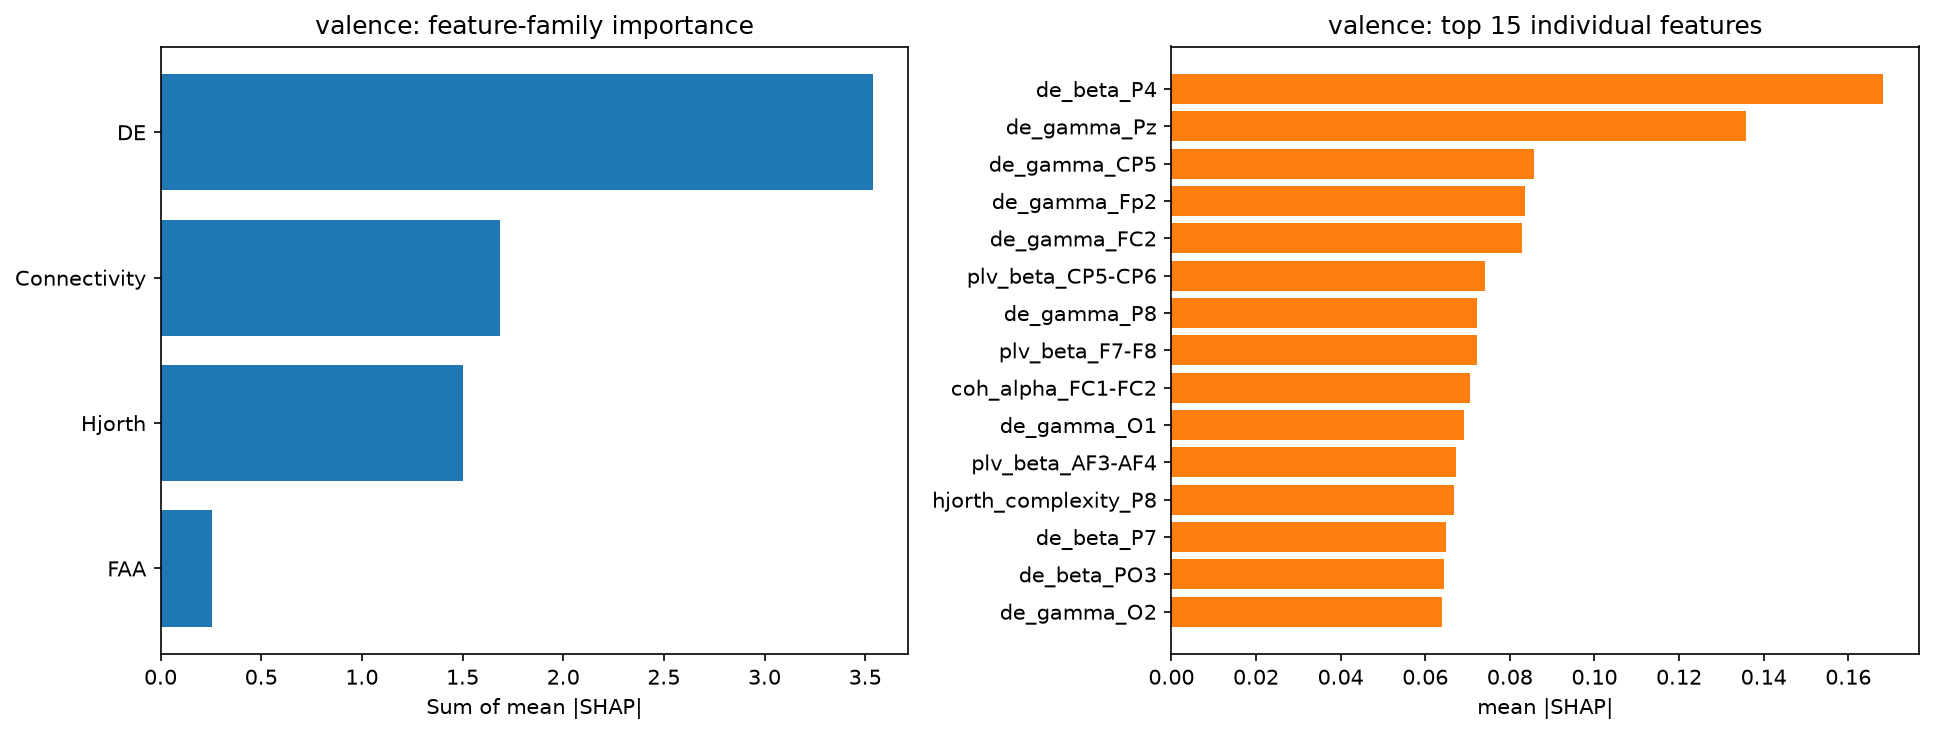
\includegraphics[width=0.8\textwidth]{track_a_shap_summary_valence.png}
\caption{SHAP summary: valence (XGBoost, Full feature set, held-out fold).}
\label{fig:shap-valence}
\end{figure}

\begin{figure}[H]
\centering
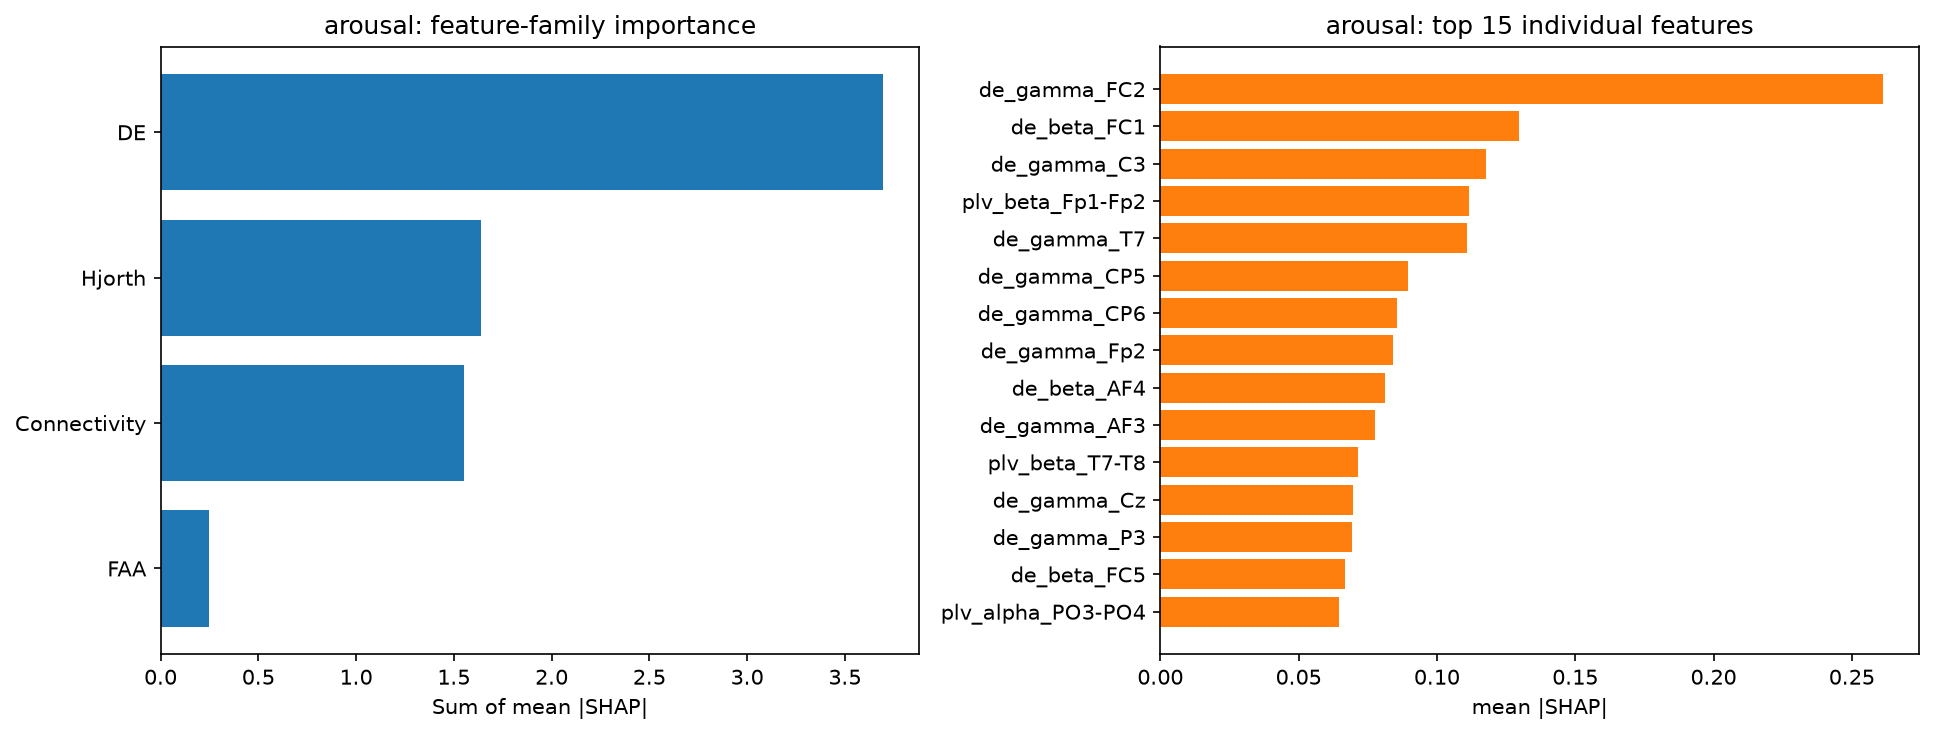
\includegraphics[width=0.8\textwidth]{track_a_shap_summary_arousal.png}
\caption{SHAP summary: arousal.}
\label{fig:shap-arousal}
\end{figure}

\begin{figure}[H]
\centering
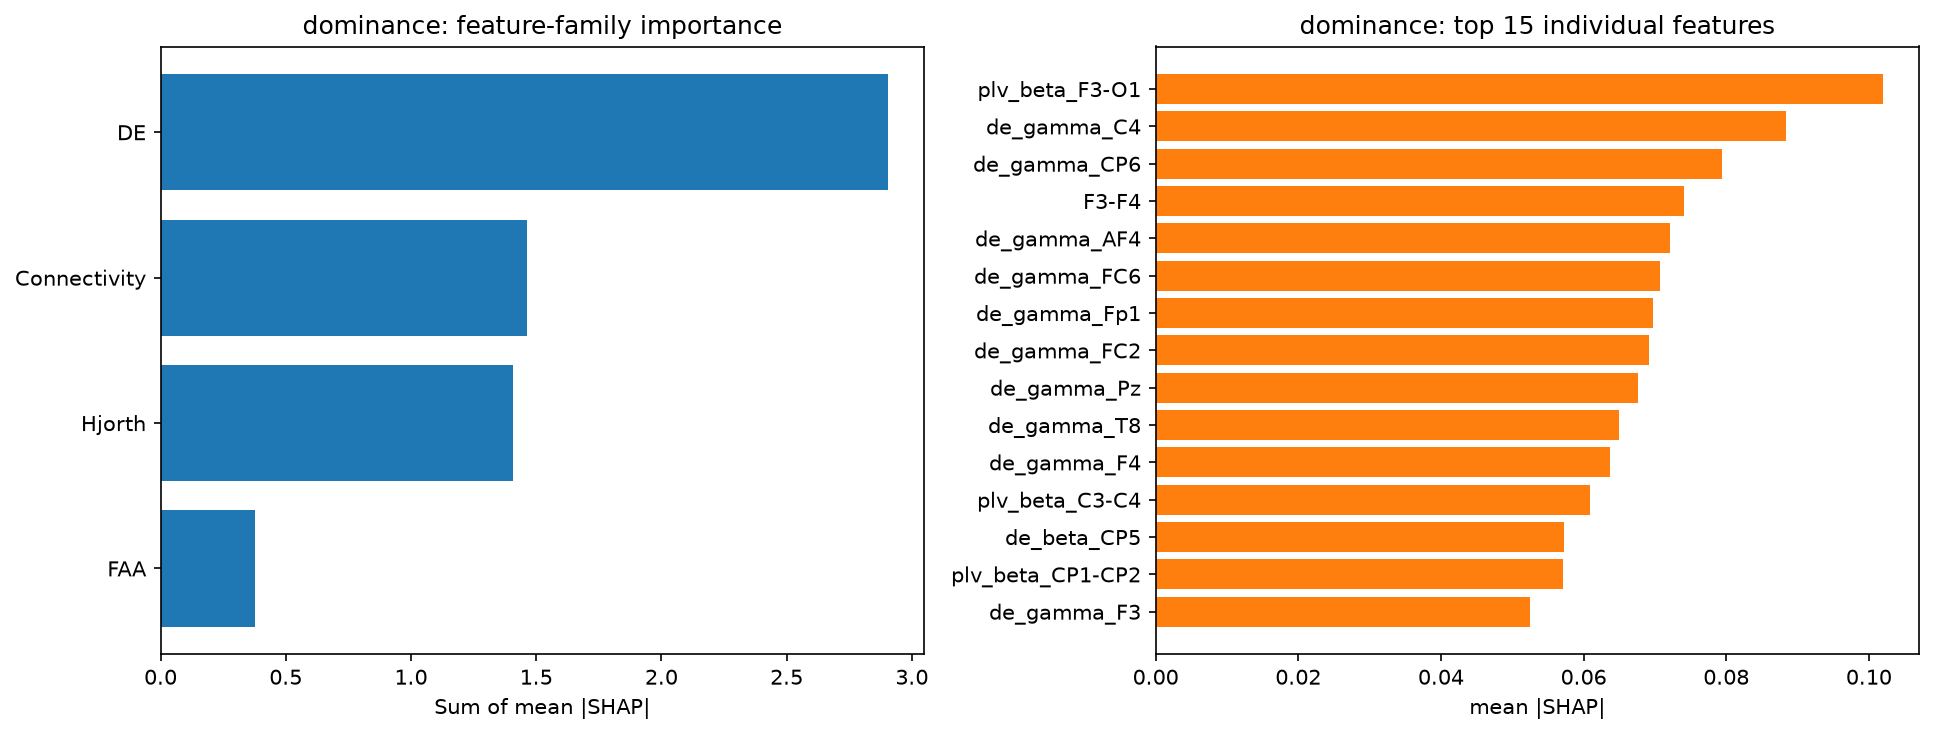
\includegraphics[width=0.8\textwidth]{track_a_shap_summary_dominance.png}
\caption{SHAP summary: dominance.}
\label{fig:shap-dominance}
\end{figure}

\begin{figure}[H]
\centering
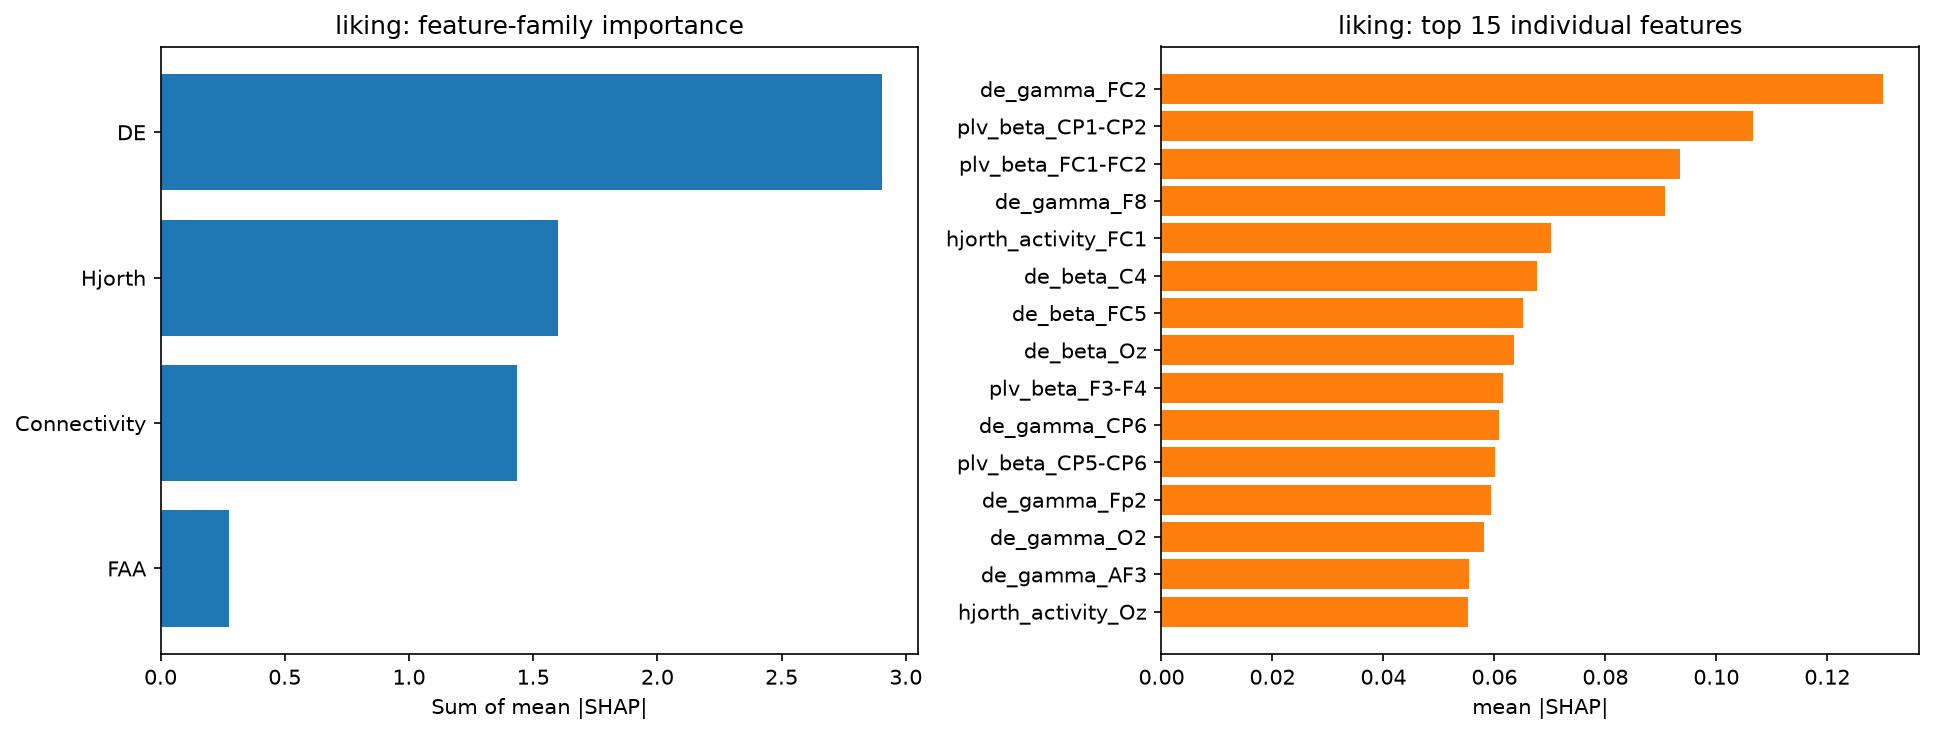
\includegraphics[width=0.8\textwidth]{track_a_shap_summary_liking.png}
\caption{SHAP summary: liking.}
\label{fig:shap-liking}
\end{figure}

\section{Does CORAL stack on top of Euclidean Alignment?}
\label{sec:s18}
I tested four conditions on the DE-only feature set: no alignment, CORAL
alone, EA alone, and EA followed by CORAL on the resulting per-fold split.
It does not stack. Mean AUC by condition: EA alone 0.523, EA+CORAL 0.514,
no-alignment baseline 0.479, CORAL alone 0.473 (the worst of the four on
this feature set). Adding CORAL on top of EA reduces AUC in 10/12 task/model
combinations (mean delta $-0.0093$). One possible reason: EA's per-subject
raw-signal whitening already removes most of the between-subject covariance
structure CORAL is also designed to correct, so CORAL's additional per-fold
alignment acts on residual structure that is mostly noise. The practical
takeaway is to use EA alone, not EA+CORAL.

\begin{table}[H]
\centering
\caption{EA+CORAL stacking: mean ROC-AUC by condition, DE-only feature
set, across 4 tasks $\times$ 3 models (12 fits)}
\label{tab:ea-coral-stacked}
\begin{tabular}{lr}
\toprule
Condition & Mean ROC-AUC \\
\midrule
none (no alignment) & 0.479 \\
CORAL alone          & 0.473 \\
EA alone             & 0.523 \\
EA + CORAL           & 0.514 \\
\bottomrule
\end{tabular}
\end{table}

\begin{figure}[H]
\centering
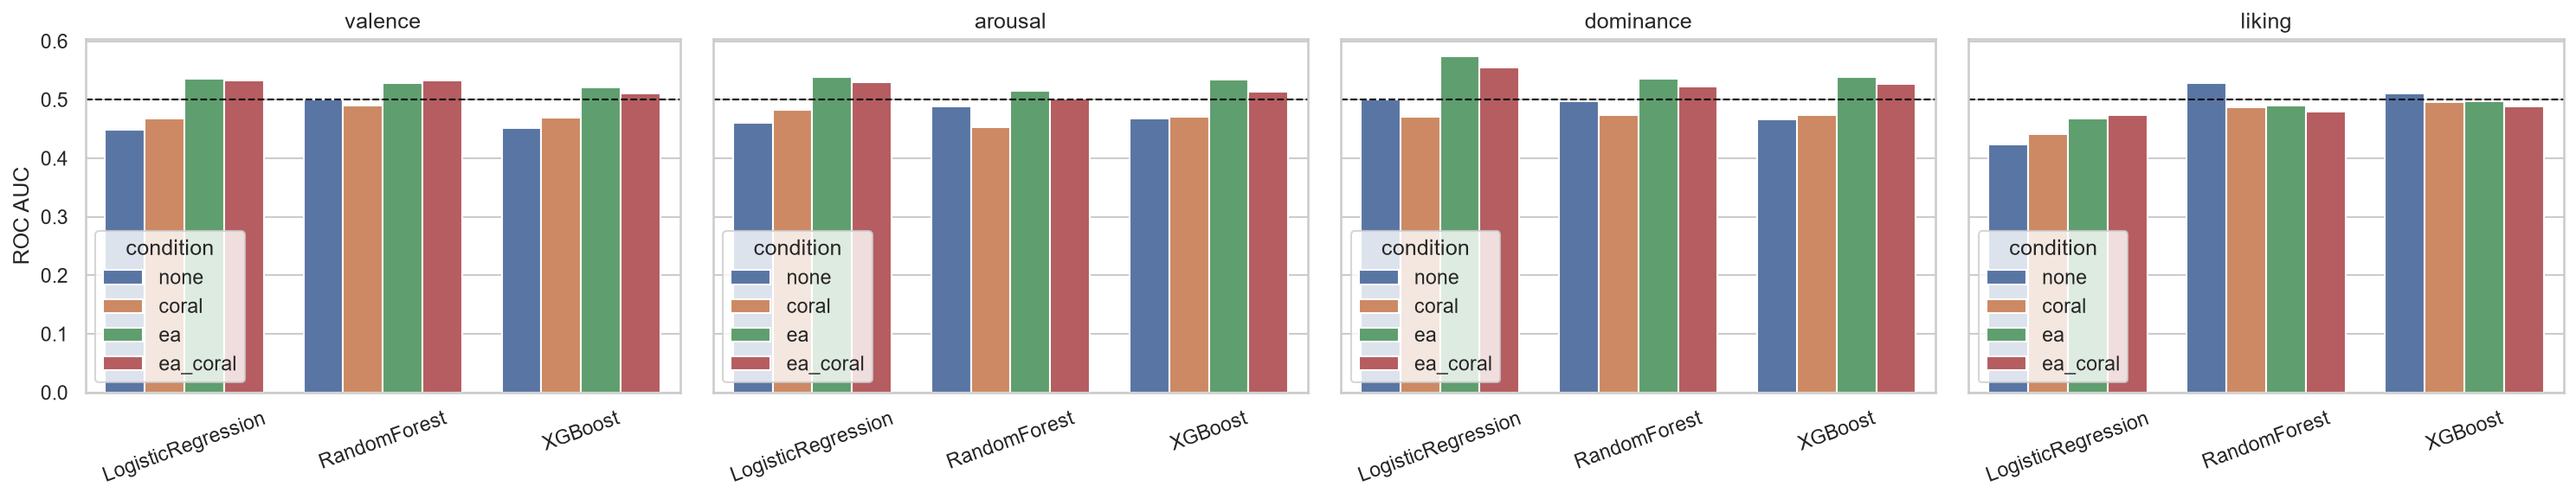
\includegraphics[width=0.85\textwidth]{track_a_ea_coral_stacked_auc.png}
\caption{EA+CORAL stacking: ROC-AUC by condition, model, and task.}
\label{fig:ea-coral-stacked}
\end{figure}

\section{EEG overview quality-control check}
\label{sec:eeg-overview}
I also built a small-multiples quality-control plot: an $8\times4$ grid, one
panel per subject, each showing all 32 channels of that subject's
baseline-normalised trial-1 EEG stacked with a fixed vertical offset, in a
single neutral ink colour. Per-channel colour-coding was deliberately
avoided: with 32 overlapping traces per panel, colour cannot carry
per-channel identity meaningfully. This is a visual sanity check, not an
analysis. It lets a reader spot subjects with obviously flat, saturated, or
anomalously noisy channels before trusting downstream numbers for them.

\begin{figure}[H]
\centering
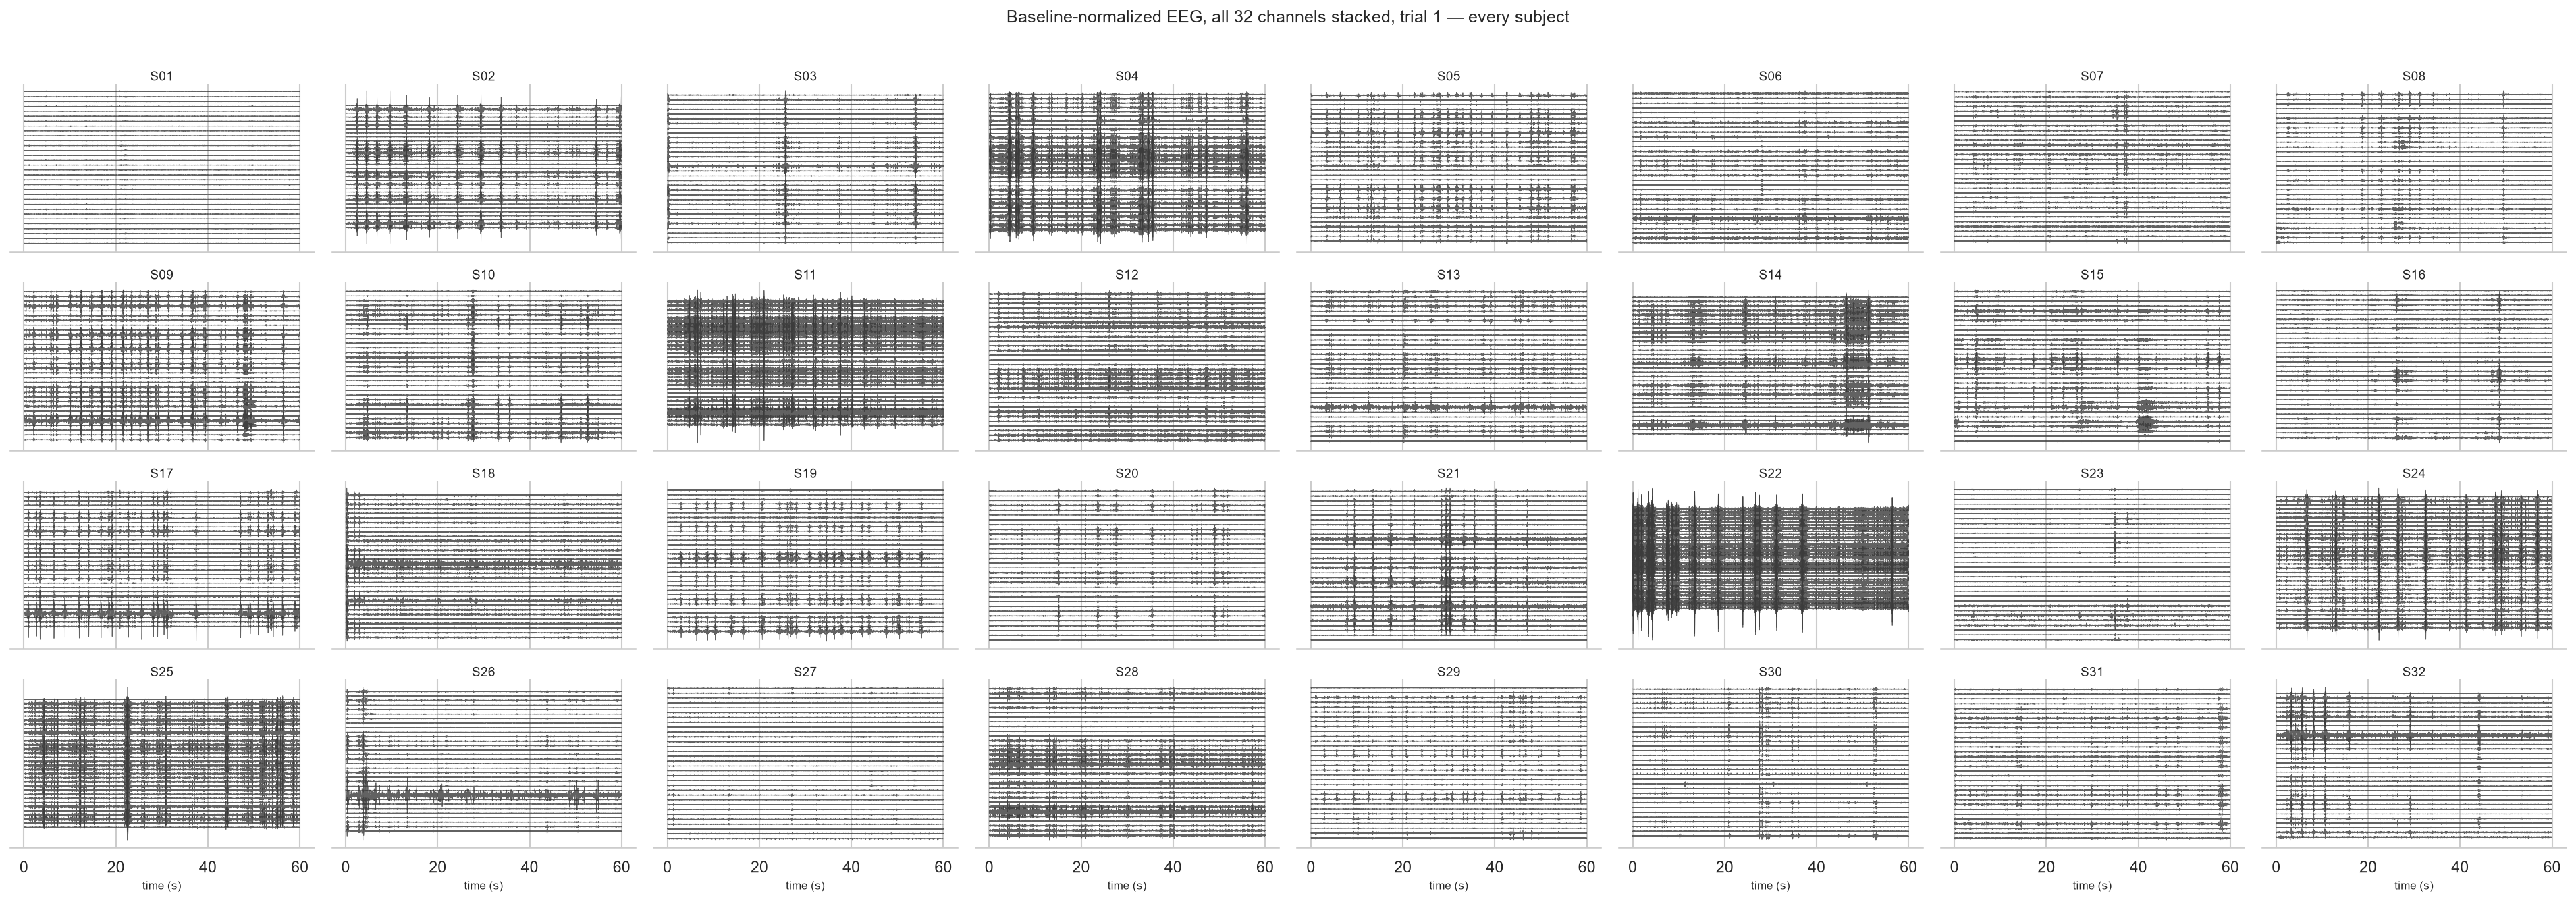
\includegraphics[width=\textwidth]{eeg_overview_all_subjects.png}
\caption{EEG overview QC grid: baseline-normalised trial-1 EEG, all 32
channels, one panel per subject (8$\times$4 grid).}
\label{fig:eeg-overview}
\end{figure}

\chapter{Appendix: Implementation Details and Companion Scripts}
\label{ch:scripts}

This appendix holds the lower-level implementation detail that
Chapter~\ref{ch:notebook} omits: function names, cache file names, and the
standalone scripts behind the experiments that were too expensive to run
inline in the notebook.

\section{Core pipeline implementation}
Two functions handle preprocessing. \texttt{load\_subject} reads a subject's
\texttt{.dat} file (a pickled dictionary of EEG data and labels).
\texttt{baseline\_normalize} subtracts the per-channel mean of the pre-trial
baseline from the stimulus signal:
\begin{lstlisting}
def load_subject(subject_id):
    fpath = DATA_DIR / f"s{subject_id:02d}.dat"
    with open(fpath, "rb") as f:
        d = pickle.load(f, encoding="latin1")
    return d["data"], d["labels"]

def baseline_normalize(trial_all_channels):
    eeg = trial_all_channels[:N_EEG_CHANNELS]
    baseline = eeg[:, :BASELINE_SAMPLES]
    signal = eeg[:, BASELINE_SAMPLES:BASELINE_SAMPLES + TRIAL_SAMPLES]
    baseline_mean = baseline.mean(axis=-1, keepdims=True)
    return (signal - baseline_mean).astype(np.float64)
\end{lstlisting}
\texttt{compute\_de\_features} band-pass filters (4th-order Butterworth,
zero-phase \texttt{sosfiltfilt}) into the four bands, reshapes each band into
15 non-overlapping 512-sample windows, and computes the Differential Entropy
of each (channel, band) pair. \texttt{make\_raw\_windows} keeps the raw
$(32, 512)$ window and standardises it per channel. A sanity check on
subject 1's first trial confirms the expected shapes: \texttt{(15, 128)} DE
features and \texttt{(15, 32, 512)} raw windows.

Configuration constants: \texttt{FS = 128}, \texttt{BASELINE\_SEC = 3},
\texttt{TRIAL\_SEC = 60}, \texttt{WINDOW\_SEC = 4}; band edges
\texttt{theta 4--8, alpha 8--13, beta 13--30, gamma 30--45\,Hz};
\texttt{LABEL\_THRESHOLD = 5.0}; \texttt{N\_EPOCHS = 40},
\texttt{BATCH\_SIZE = 128}, \texttt{PATIENCE = 8} for Track B training.
Track B's \texttt{subject\_independent\_split} performs a nested
\texttt{GroupShuffleSplit} for the 70/15/15 split; \texttt{train\_torch\_model}
wraps the \texttt{AdamW} + \texttt{ReduceLROnPlateau} + mixed-precision
training loop described in Section~\ref{sec:s6}.

The main windowed dataset is cached to
\texttt{processed\_cache/deap\_windows\_4s\_32subj\_v2.npz}; the extended
295-feature set (Section~\ref{sec:s9}) to
\texttt{deap\_features\_ext\_v1.npz}; the 50\%-overlap window variant
(Section~\ref{sec:s11}) to \texttt{deap\_windows\_4s\_overlap50\_32subj\_v1.npz}.
Caches are schema-versioned so a stale cache from before dominance/liking
were tracked is never silently reused.

\section{Feature/dataset builders}
\begin{description}
  \item[\texttt{dl\_models.py}] Canonical PyTorch definitions of EEGNet,
        ShallowConvNet, CNN-LSTM, and TSception, plus the hemisphere-pair
        channel indices TSception needs. Imported by every
        \texttt{track\_b\_*.py} script so the architectures are defined
        exactly once, not re-implemented per script.
  \item[\texttt{rich\_features.py}] Implements Hjorth parameters
        (\texttt{compute\_hjorth}), frontal/hemispheric alpha asymmetry
        (\texttt{compute\_alpha\_asymmetry}), and PLV/coherence connectivity
        (\texttt{compute\_connectivity}, via a from-scratch Hilbert-transform
        phase-locking-value computation and a Welch-style
        magnitude-squared-coherence estimator). Includes a
        \texttt{if\_\_name\_\_=="\_\_main\_\_"} self-test against synthetic
        data (shape checks, $[0,1]$-boundedness for PLV/coherence, and an
        index-math cross-check for FAA) that must pass before the module is
        trusted for the real build.
  \item[\texttt{build\_extended\_features.py}] Runs \texttt{rich\_features.py}
        (plus DE) over all 32 DEAP subjects, producing
        \texttt{deap\_features\_ext\_v1.npz} (295-dim Full feature set,
        19{,}200 windows). Its DE computation is verified to match the
        original cache byte-for-byte before the richer features are trusted.
  \item[\texttt{build\_overlap\_windows.py}] Rebuilds the raw-window Track B
        dataset with 50\% stride overlap
        (\texttt{deap\_windows\_4s\_overlap50\_32subj\_v1.npz}, 37{,}120
        windows), for Section~\ref{sec:s11}.
  \item[\texttt{build\_raw\_ratings.py}] Extracts the raw continuous 1--9
        SAM ratings per window, row-aligned 1:1 with the extended feature
        cache (verified via an explicit \texttt{groups} array equality
        assertion), for Section~\ref{sec:s14}'s label-cleanup variants.
\end{description}

\section{Track A companion scripts}
\begin{description}
  \item[\texttt{track\_a\_ablation.py}] Section~\ref{sec:s9}: 6 feature-set
        combinations $\times$ 3 models $\times$ 4 tasks, \texttt{GroupKFold(5)}.
  \item[\texttt{track\_a\_repeated\_nested\_cv.py}] Section~\ref{sec:s10}:
        5$\times$-repeated \texttt{GroupKFold} for all 6 models (with a
        custom subject-relabeling generator, \texttt{repeated\_group\_}\linebreak
        \texttt{kfold\_splits}, since \texttt{sklearn} has no
        \texttt{RepeatedGroupKFold}) plus nested
        \texttt{GroupKFold(3)}/\texttt{RandomizedSearchCV} hyperparameter
        search for XGBoost and RandomForest.
  \item[\texttt{track\_a\_label\_cleanup.py}] Section~\ref{sec:s14}: the
        three label-binarisation variants (\texttt{raw\_threshold},
        \texttt{per\_subject\_z}, \texttt{drop\_middle}).
  \item[\texttt{track\_a\_calibration\_loso.py}] Section~\ref{sec:s15}: true
        32-fold LOSO with an 80/20 per-subject eval/calibration trial split
        and XGBoost warm-start (\texttt{xgb\_model=} continuation boosting).
  \item[\texttt{track\_a\_significance\_test.py}] Section~\ref{sec:s16}.1:
        300-permutation, trial-within-subject label-shuffle null-distribution
        test, parallelised across CPU cores with \texttt{joblib.Parallel}.
  \item[\texttt{track\_a\_domain\_alignment.py}] Section~\ref{sec:s16}.2:
        CORAL alignment (\texttt{coral\_align}, via
        \texttt{\_sym\_matrix\_power} eigendecomposition).
  \item[\texttt{track\_a\_riemannian\_alignment.py}] Section~\ref{sec:s17}.1:
        Euclidean Alignment (\texttt{euclidean\_align}), operating on raw
        windows before DE recomputation.
  \item[\texttt{track\_a\_shap\_diagnostic.py}] Section~\ref{sec:s17}.5:
        \texttt{shap.TreeExplainer} on one representative fold per task,
        aggregated by feature and by family, with bar-chart figures saved
        per task.
  \item[\texttt{track\_a\_ea\_coral\_stacked.py}] Section~\ref{sec:s18}: the
        4-condition (\texttt{none}/\texttt{coral}/\texttt{ea}/\texttt{ea\_coral})
        stacking test, re-implementing both \texttt{euclidean\_align} and
        \texttt{coral\_align} locally so this script is self-contained.
\end{description}

\section{Track B companion scripts}
\begin{description}
  \item[\texttt{track\_b\_repeated.py}] Section~\ref{sec:s11}: 5-seed
        repeated subject-independent splits, both window variants, all 4
        architectures $\times$ 4 tasks (160 runs).
  \item[\texttt{track\_b\_domain\_adversarial.py}] Section~\ref{sec:s16}.3:
        \texttt{GradReverse} autograd function, \texttt{EEGNetDANN} (reuses
        EEGNet's conv blocks, adds a GRL + domain-classifier branch), and
        the Ganin \& Lempitsky progressive-$\lambda$ training loop.
  \item[\texttt{track\_b\_ssl\_pretrain.py}] Section~\ref{sec:s17}.2:
        \texttt{EEGNetSSL} (shares EEGNet's trunk, regression head for the
        DE-prediction pretext task), a 15-epoch label-free pretraining
        stage, then fine-tuning; the training/val/test split is computed
        once and reused across all four tasks (compute optimisation, not a
        methodological shortcut, since the split depends only on
        \texttt{groups}/\texttt{seed}, not on labels).
  \item[\texttt{track\_b\_auc\_maximization.py}] Section~\ref{sec:s17}.3:
        \texttt{auc\_margin\_loss}, a drop-in loss-function swap with
        everything else (model, split, seed) held identical to the
        cross-entropy baseline.
  \item[\texttt{track\_b\_test\_time\_adaptation.py}] Section~\ref{sec:s17}.4:
        \texttt{reset\_bn\_for\_adaptation} (zeroes BatchNorm running stats,
        sets momentum to \texttt{None} for a true cumulative average) and
        \texttt{adabn\_predict\_one\_subject} (2 label-free adaptation
        epochs per test subject, under \texttt{torch.no\_grad()}).
\end{description}

\section{Cross-corpus scripts}
See Section~\ref{sec:seed-iv-adapter} for \texttt{base.py},
\texttt{seed\_adapter.py}, and \texttt{run\_cross\_corpus.py}.

\section{Notebook-authoring scripts}
A handful of one-off scripts were used to author the notebook's cells during
earlier stages of the project. They are not part of the reproducible-results
path.

\section{Script/notebook execution map}
\label{sec:execution-map}
There is no automation wiring the scripts and the notebook together -- no
notebook cell calls a script, and no script calls the notebook. Every
Tier-1 companion script above is run manually from a terminal, writes a
\texttt{.npz}/\texttt{.csv}/\texttt{.png} file to \texttt{processed\_cache/}
or \texttt{results/}, and a separate notebook cell later reads that file
back in. \texttt{script\_notebook\_execution\_map.txt}, at the repository
root, is the hand-verified record of that manual wiring: it groups the
builders into a Tier 0 (three scripts that turn the raw DEAP \texttt{.dat}
files into the \texttt{processed\_cache/*.npz} caches every later step reads)
and a Tier 1 (every companion script, each mapped to the exact notebook
section and cell range that consumes its output), notes which caches a
script depends on before it will run, and ends with a recommended
clean-checkout run order. It also flags a concrete rough edge: three of the
Tier-0 builders (\texttt{build\_extended\_features.py},
\texttt{build\_raw\_ratings.py}, \texttt{build\_overlap\_windows.py}) still
hardcode an old \texttt{D:/EEG/...} path for \texttt{DATA\_DIR}/\texttt{CACHE\_DIR}
from an earlier stage of the project, unlike
\texttt{track\_a\_significance\_test.py}, which was already migrated to a
relative, repository-root-based path; those three need that path fixed (or
need to be run from the original location) before a clean checkout can
reproduce their caches. The map is generated by inspecting the current
repository state rather than hand-maintained prose, so it is the more
reliable of the two if a script or notebook cell is ever added, removed, or
renamed after this report is written.

\chapter{Literature Review and Bibliography}
\label{ch:literature}

\section{Corpus}
\texttt{papers\_EEG/} contains 32 papers I reviewed for this project, each
renamed to a descriptive title. Two plain-text files at the repository root
track this corpus outside of \LaTeX: \texttt{citations.txt} is the flat
citation list (the source for the \texttt{bibitem} entries in this chapter's
bibliography), and \texttt{literature\_log.txt} is a per-paper log of what
each paper covers and, where applicable, which section of this report it
fed into; it was reconstructed in one pass late in the project by reading
all 32 papers directly (Chapter~\ref{ch:challenges} discusses why).
Table~\ref{tab:papers-cited} lists the 13 with an explicit, documented role
in an experiment: named as the specific motivation behind a specific
intervention.

\begin{longtable}{p{3.4cm}p{2.4cm}p{6.8cm}}
\caption{Papers with an explicit, documented contribution to this project}
\label{tab:papers-cited} \\
\toprule
Paper & Used in & Why \\
\midrule
\endfirsthead
\toprule
Paper & Used in & Why \\
\midrule
\endhead
\citet{khan_ndreviewfailures} &
Section~\ref{sec:s16-1} &
Documents that DEAP pipelines can look deceptively strong under leaky
evaluation, even on a label-randomised control. This motivated building a
permutation-null significance test for my own \texttt{GroupKFold} protocol. \\
\addlinespace
\citet{sarafraz2022domain} &
Sections~\ref{sec:s16-2}, \ref{sec:s16-3}, \ref{sec:s17-1} &
Surveys CORAL and Euclidean Alignment as standard, cheap, unsupervised
domain-adaptation remedies for distribution shift, and is one of several
sources converging on adversarial subject-invariance (DANN). \\
\addlinespace
\citet{ye2024dsagc} &
Sections~\ref{sec:s16-2}, \ref{sec:s17-1} &
Reports plain CORAL reaching roughly 65--70\% under LOSO on SEED, where
untransformed features stay under 60\%: the empirical precedent that
motivated testing CORAL and EA here, though my own CORAL result did not
replicate that scale of gain. \\
\addlinespace
\citet{zhang2022parse} &
Section~\ref{sec:s16-3} &
One of several independently-converging sources recommending a
gradient-reversal-layer domain discriminator for subject-invariant EEG
representation learning. \\
\addlinespace
\citet{li2022tutorial} &
Section~\ref{sec:s16-3} &
Same DANN motivation as above. \\
\addlinespace
\citet{liu2024gnnsurvey} &
Section~\ref{sec:s16-3} &
Same DANN motivation as above. \\
\addlinespace
\citet{liu2026brainsci} &
Section~\ref{sec:s16-3} &
Same DANN motivation as above. \\
\addlinespace
\citet{sreehari2026review} &
Section~\ref{sec:s16-3} &
Names over-aggressive alignment collapsing class structure as a documented
failure pattern in unsupervised domain adaptation, matched by my own DANN
arousal/dominance collapse and used to interpret that result. \\
\addlinespace
\citet{wang2024cascaded} &
Section~\ref{sec:s17-2} &
The one paper in the review that evaluated LOSO on DEAP itself while
beating domain-adaptation baselines: the strongest outside evidence that a
pretraining stage, rather than a training-time loss or architecture change,
could move subject-independent AUC. \\
\addlinespace
\citet{weng2023sslsurvey} &
Section~\ref{sec:s17-2} &
Corroborating survey context for the SSL-pretraining design. \\
\addlinespace
\citet{xiao2024aucmax} &
Section~\ref{sec:s17-3} &
The most directly on-metric deferred idea: my headline metric is ROC-AUC,
so a loss that directly targets AUC, rather than per-sample cross-entropy,
is a natural, cheap intervention to test. \\
\addlinespace
\citet{imtiaz2025sourcefree} &
Section~\ref{sec:s17-4} &
Surveys the source-free UDA family, of which AdaBN is the cheapest,
most-established member, as a natural target-aware follow-up to DANN. \\
\addlinespace
\citet{mouazen2025hybrid} &
Section~\ref{sec:s17-5} &
Motivated logging the SHAP interpretability diagnostic as a cheap check on
whether near-chance models lean on plausible or noise-like features. \\
\bottomrule
\end{longtable}

\section{Papers reviewed but not tied to a specific experiment}
\label{sec:literature-gap}
I list these 19 papers separately, rather than silently dropping them from
the corpus once they did not produce a script, for the same transparency
reason the retracted permutation-test claim in Section~\ref{sec:s16-1} is
kept rather than deleted: a literature review that only shows the sources
that paid off gives a misleading picture of how much reading actually went
into the design decisions above, and hides the fact that several plausible
directions (GAN/diffusion-based data augmentation, graph-neural-network and
transformer architectures, contrastive self-supervised pretraining beyond
the one variant I did implement) were considered and set aside rather than
never considered at all. The remaining 19 papers in the corpus were part of
the same review pass (EEG-emotion surveys, domain-adaptation and
generalisation methods, contrastive/self-supervised pretraining,
GAN/diffusion augmentation, and DEAP-specific methodology critiques) but did
not drive a specific implemented experiment, generally because they targeted
a different dataset, required an architecture change larger than a
retrofit onto the ten base models already built, or converged on a
recommendation (e.g.\ domain adaptation, self-supervised pretraining) that
an already-cited paper in Table~\ref{tab:papers-cited} had independently
motivated with a clearer, more directly applicable empirical precedent:
\citet{liu2022spatiotemporal}, \citet{qiao2022cnn3d},
\citet{menezes2017virtual}, \citet{xu2022amdet}, \citet{guo2023memhacl},
\citet{kan2022sgmc}, \citet{siddhad2025diffusion},
\citet{liu2024graphperspective}, \citet{liu2025scmm}, \citet{wang2025fourier},
\citet{gong2025lel}, \citet{dolgopolyi_ndeeplearning},
\citet{purwar2026threeway}, \citet{kalashami2022augmentation},
\citet{pan2021gan}, \citet{liu2024ertnet}, \citet{hamzah2024heliyon},
\citet{azar2024fuzzy}, and \citet{karthiga2024metaheuristic}. They are
listed here as background and related work rather than trimmed from the
corpus, since they informed my sense of the field even where they did not
map to a specific script.

\chapter{Consolidated Results}
\label{ch:results}

Chapter~\ref{ch:notebook} presents each experiment's numbers embedded in its
own methods and discussion, which is the right place to read any one result
in context but makes it hard to see the project's overall shape at a glance:
whether the interventions cluster into a few that worked and many that
did not, or whether the effects are uniformly small throughout. Table
\ref{tab:master} consolidates the headline AUC numbers across every
experiment in the notebook, in chronological/section order, specifically to
make that shape visible in one place. All numbers are mean ROC-AUC unless
noted; ``$\Delta$'' is the change versus that experiment's own stated
control condition. Reading down the Verdict column, only two of the
fourteen listed interventions earn an unqualified positive verdict
(Euclidean Alignment and, on the one task it targets, the AUC-margin loss);
the great majority land on ``no stable effect,'' ``inconsistent, not real
gain,'' or an explicit negative (DANN's arousal/dominance collapse, EA+CORAL
underperforming EA alone). That imbalance, more than any single row, is the
table's real content: it is a compact visual record of the same
negative-result pattern that Section~\ref{sec:s13} and Chapter
\ref{ch:model-analysis} argue for in prose, now readable as fourteen
data points rather than as an argument that has to be taken on trust.

\begin{longtable}{p{5.5cm}p{2.3cm}p{2.1cm}p{4.3cm}}
\caption{Master results table} \label{tab:master} \\
\toprule
Experiment (section) & Best/observed AUC & $\Delta$ vs.\ control & Verdict \\
\midrule
\endfirsthead
\toprule
Experiment (section) & Best/observed AUC & $\Delta$ vs.\ control & Verdict \\
\midrule
\endhead
Track A best model (\S5) & 0.501--0.534 & n/a & near chance \\
Track B best model (\S6) & 0.475--0.607 & n/a & near chance, mixed by task \\
Feature-set ablation (\S9) & 0.478--0.494 (means) & $\le0.016$ across sets & no feature set helps \\
Repeated GroupKFold (\S10) & 15/24 CIs contain 0.5 & n/a & mostly chance-consistent \\
Nested CV (\S10) & 0.454--0.524 & $\approx0$ vs.\ fixed HP & tuning is not the bottleneck \\
Window overlap (\S11) & 0.483 vs.\ 0.498 & $+0.015$ & inconsistent, not real gain \\
Cross-corpus DEAP baseline (\S12) & 0.452 & n/a & weakest of the three settings \\
Cross-corpus zero-shot (\S12) & 0.517 & $+0.065$ vs.\ DEAP baseline & modest, above chance \\
Cross-corpus SEED-IV LOSO (\S12) & 0.673 & $+0.221$ vs.\ DEAP baseline & moderate signal \\
Label cleanup, per\_subject\_z (\S14) & 0.514 (mean) & $+0.031$ vs.\ raw & modest, confounded by rebalancing \\
Calibration, arousal (\S15) & 0.577 & $+0.071$ vs.\ zero-shot & modest personalisation effect \\
Permutation test, dominance (\S16.1) & 0.561 & $z=+2.18$, $p=0.0199$ & significant but small, not Bonferroni-robust \\
Permutation test, others (\S16.1) & 0.437--0.458 & $p=0.877$--$0.997$ & not distinguishable from null \\
CORAL (\S16.2) & mean $\Delta+0.0059$ & 8/12 up, 4/12 down & no stable effect \\
DANN, valence/liking (\S16.3) & $+0.039$/$+0.050$ & n/a & small gains \\
DANN, arousal/dominance (\S16.3) & $-0.216$/$-0.149$ & n/a & \textbf{collapse} \\
Euclidean Alignment (\S17.1) & mean $\Delta+0.044$ & 10/12 up & \textbf{strongest effect overall} \\
SSL pretraining (\S17.2) & $+0.074$/$+0.100$ (val/lik) & $-0.082$/$-0.053$ (aro/dom) & bimodal task split \\
AUC-margin loss (\S17.3) & $+0.083$ (valence) & mixed elsewhere & mechanistically understood win \\
AdaBN (\S17.4) & $+0.082$ (liking) & $-0.101$/$-0.063$ (aro/dom) & net negative \\
SHAP diagnostic (\S17.5) & n/a & n/a & diffuse importance, FAA weakest \\
EA+CORAL stacking (\S18) & EA 0.523 vs.\ EA+CORAL 0.514 & $-0.0093$ & \textbf{does not stack; use EA alone} \\
\bottomrule
\end{longtable}

\section{Figures}
All 24 figures in \texttt{results/figures/} are embedded in place in
Chapter~\ref{ch:notebook}, alongside the section that produced them (see
List of Figures, p.~\pageref{fig:class-balance}, for the full index). The
most important for a final report remain \texttt{class\_balance.png}
(Fig.~\ref{fig:class-balance}, \S4),
\texttt{track\_a\_accuracy.png}/\texttt{combined\_accuracy\_comparison.png}
(Figs.~\ref{fig:track-a-accuracy}/\ref{fig:combined-accuracy}, \S5--7),
\texttt{track\_a\_repeated\_cv\_auc\_ci.png} (Fig.~\ref{fig:repeated-cv},
\S10), \texttt{track\_a\_riemannian\_alignment\_auc.png}
(Fig.~\ref{fig:ea}, \S17.1, the strongest result),
\texttt{track\_a\_ea\_coral\_stacked\_auc.png}
(Fig.~\ref{fig:ea-coral-stacked}, \S18), and
\texttt{cross\_corpus\_deap\_seediv.png} (Fig.~\ref{fig:cross-corpus},
\S12).

\chapter{Model-by-Model Analysis}
\label{ch:model-analysis}

Chapters~\ref{ch:notebook} and \ref{ch:results} report what each of the ten
models scored. This chapter looks at why, for each model, at the level of
inductive bias, capacity, and training procedure. These are my working
hypotheses for each score, not confirmed mechanisms: none of them were
tested directly against an alternative explanation, and most of the
differences between models are small relative to fold-to-fold noise. Where
an effect is large enough to be worth a fuller explanation, I say so and
note it as a hypothesis; where a difference is comparable to normal
fold-to-fold variation, I say that instead of inventing a story for it.

\section{A shared ceiling: what every model is fighting against}
\label{sec:ma-shared}
Five properties of the DEAP setup apply to all ten models and are worth
holding in mind when reading any individual score:
\begin{itemize}
  \item Class imbalance is task-dependent and interacts with accuracy.
        Valence (21.0\% high) and arousal (23.3\% high) reward any model
        that leans on the majority class; dominance (60.9\% high) and
        liking (66.5\% high) are close enough to balanced that accuracy and
        AUC tend to agree more (Section~\ref{sec:s4}). A model's accuracy on
        valence/arousal is only informative once checked against its AUC:
        high accuracy with AUC near 0.5 is the majority-class-collapse
        signature discussed in Section~\ref{sec:s8}.
  \item Only 32 subjects supply the grouping variable. Under
        \texttt{GroupKFold(5)}/\texttt{GroupShuffleSplit}, each held-out
        fold is about 6--7 entire subjects the model has never seen. With
        this few groups, between-subject variance in raw EEG amplitude,
        electrode impedance, and baseline arousal state is a large fraction
        of total variance, large enough that some fold-to-fold swings are
        driven more by which subjects landed in which fold than by any
        model property. This is a background noise floor that no
        architecture change removes, and it is a large part of why
        Section~\ref{sec:s10}'s repeated $5\times5$ GroupKFold shows 15/24
        95\% confidence intervals still spanning chance.
  \item The labels are self-report, thresholded 1--9 ratings, not a
        physiological ground truth. Section~\ref{sec:s14}'s label-cleanup
        ablation shows that even changing how the same raw ratings are
        binarised moves mean AUC by at most $+0.031$, so no model, however
        expressive, can be expected to find much more signal than the label
        construction itself contains.
  \item Track A and Track B are evaluated under different variance regimes.
        Track A's numbers are 5-fold \texttt{GroupKFold} means; Track B's
        headline numbers (Table~\ref{tab:track-b-best}) are single-split
        point estimates, so an individual Track B score is noisier and more
        fold-luck-dependent than a Track A one (Section~\ref{sec:s11}'s
        repeated splits give mean AUC 0.483 non-overlap, consistent with the
        single-split numbers here).
  \item All 32 DEAP subjects watched the same 40 stimulus videos. Any
        component of arousal or valence that is driven by the stimulus
        rather than the person is, in effect, partially shared across
        subjects even under a leakage-free \texttt{GroupKFold} split: no
        subject's windows leak, but the video each window comes from is
        seen by the model during training via other subjects' reactions to
        it. This may be part of why arousal tends to score a little better
        than the other three tasks for several models, though all four
        stay close to chance overall, without implying any actual data
        leakage.
\end{itemize}

\section{Track A: classical models on DE features}
\label{sec:ma-tracka}
All six models share the same 128-dim Differential Entropy input, the same
standard-scaling preprocessing, and the same 5-fold \texttt{GroupKFold}
protocol (Section~\ref{sec:s5}), so differences between them are
attributable to model family, not to differences in the data they see
(except SVM-RBF's 8000-sample training cap). Table~\ref{tab:ma-tracka-auc}
collects every model's mean ROC-AUC on every task.

\begin{table}[H]
\centering
\caption{Track A -- every classical model's mean ROC-AUC, all four tasks
(5-fold GroupKFold)}
\label{tab:ma-tracka-auc}
\begin{tabular}{lrrrr}
\toprule
Model & Valence & Arousal & Dominance & Liking \\
\midrule
LogisticRegression & 0.449 & 0.461 & 0.500 & 0.424 \\
kNN ($k=15$)        & 0.465 & 0.495 & 0.501 & 0.531 \\
RandomForest (300 trees) & 0.501 & 0.489 & 0.497 & 0.528 \\
SVM-RBF ($C=10$)    & 0.500 & 0.450 & 0.513 & 0.534 \\
XGBoost (depth 6)   & 0.455 & 0.483 & 0.473 & 0.505 \\
MLP (128,64)        & 0.457 & 0.439 & 0.493 & 0.488 \\
\bottomrule
\end{tabular}
\end{table}

\subsection{Logistic Regression}
\label{sec:ma-lr}
The only strictly linear model in the comparison, and the one I reused as
the fast proxy in the permutation significance test (Section~\ref{sec:s16-1})
and inside CORAL alignment (Section~\ref{sec:s16-2}). Its AUC sits at or
below chance on three of four tasks (0.449 valence, 0.461 arousal, 0.424
liking, the single worst score of any model on any task in Track A) and
only reaches 0.500 on dominance. One possible reason: the SHAP diagnostic
(Section~\ref{sec:s17-5}) finds class-relevant structure diffuse across
dozens of features with no single dominant direction, and a linear
hyperplane has limited ability to combine that kind of structure into a
useful score. Liking's especially poor score, meaningfully below 0.5, is
consistent with this model's role as the null-hypothesis proxy in
Section~\ref{sec:s16-1}: it can be pushed to the wrong side of chance by
fold-to-fold subject swapping. It is also the fastest model in Track A.

\subsection{k-Nearest Neighbours}
The only non-parametric model in the comparison: it classifies by majority
vote among each test point's 15 nearest neighbours in 128-dimensional space.
It is never the single best model in Table~\ref{tab:ma-tracka-auc}, but it
is the best of the six on arousal (0.495) and the second-best on liking
(0.531, behind SVM-RBF). One possible reason is that kNN has no
training-time optimisation that can overfit a training fold's particular
mix of subjects, since its only free parameter is $k$, fixed in advance.
It does not lead on valence (0.465) or dominance (0.501); the differences
between kNN and the other classical models on those two tasks are small
enough to be within normal fold-to-fold variation rather than a
model-specific effect worth explaining further.

\subsection{Random Forest}
\label{sec:ma-rf}
With scikit-learn's default unlimited tree depth, Random Forest is the
single best model by AUC on valence (0.501) and by a wide margin the best by
accuracy on every task (0.779 valence, 0.767 arousal, 0.577 dominance, 0.643
liking). This accuracy/AUC split is one of the clearest illustrations in
this report of the majority-class-collapse pattern discussed in
Section~\ref{sec:s8}: bagged trees can find splits that predict the
majority class on valence/arousal with high accuracy without needing the
minority class to be separable. Averaging over 300 trees also gives it the
tightest accuracy variance in Track A, which makes it look stable, but
stability of an accuracy number built partly on base-rate exploitation is
not the same as stability of a real discriminative signal; its AUC
(0.489--0.501) is unremarkable once that base rate is accounted for.

\subsection{Support Vector Machine (RBF kernel)}
Trained on at most 8000 randomly subsampled windows per fold, SVM-RBF is
the best model by AUC on two of four tasks: dominance (0.513) and liking
(0.534, the single highest AUC anywhere in Track A). It is also the
slowest model by 1--2 orders of magnitude, and has the lowest accuracy of
any model on valence (0.676) and arousal (0.691): it is the one classical
model that consistently avoids leaning on the majority class, plausibly
because its internal probability calibration smooths output scores away
from the overconfident majority-class predictions that inflate other
models' accuracy without inflating their AUC. The 8000-sample cap is worth
flagging as a real confound: on valence and arousal, where the full
training fold has over 15{,}000 windows, SVM-RBF sees under 60\% of the
available data, which may cost it AUC on exactly the two tasks where it
under-performs kNN and Random Forest.

\subsection{XGBoost}
\label{sec:ma-xgb}
XGBoost is never the best Track A model on any task (0.455 valence, 0.483
arousal, 0.473 dominance, 0.505 liking), despite being the model I chose to
represent Track A in the feature-set ablation (Section~\ref{sec:s9}) and
the SHAP diagnostic (Section~\ref{sec:s17-5}). Gradient boosting fits trees
sequentially to residual error, which can make it more prone than bagging
to chasing patterns specific to a training fold's particular subject mix.
Consistent with this, nested hyperparameter search (Section~\ref{sec:s10})
barely moves its AUC (dominance: 0.494 tuned vs.\ 0.473 fixed
hyperparameters), so tuning does not appear to be the main bottleneck.
XGBoost is the cheapest model per fit after kNN, which is why I used it for
the many companion scripts that run hundreds of fits (ablation,
label-cleanup, calibration LOSO).

\subsection{MLP (shallow feed-forward network)}
The only model in Track A with a trainable nonlinear architecture, and it
is nonetheless never the best model on any task and is the single worst
model on arousal (0.439, below even Logistic Regression's 0.461). This is a
meaningful negative result on its own: if two extra hidden layers on the
same 128 DE features cannot beat a linear model, the ceiling is unlikely to
be that classical features need a nonlinear decision function, which lines
up with Section~\ref{sec:s9}'s finding that richer feature sets do not move
AUC either. Its accuracy variance on valence is the widest in Track A,
consistent with early stopping shrinking its effective training data.

\section{Track B: deep models on raw EEG windows}
\label{sec:ma-trackb}
All four architectures share the same raw, baseline-normalized 32-channel
$\times$ 512-sample (4\,s) input, the same \texttt{AdamW} +
\texttt{ReduceLROnPlateau} + early-stopping (patience 8) training loop, and
the same single 70/15/15 subject-independent split (Section~\ref{sec:s6}),
so differences are attributable to architecture and parameter count.
Table~\ref{tab:ma-trackb-auc} collects every model's ROC-AUC on every task.

\begin{table}[H]
\centering
\caption{Track B -- every deep model's ROC-AUC, all four tasks (single
subject-independent split)}
\label{tab:ma-trackb-auc}
\begin{tabular}{lrrrrr}
\toprule
Model & Params & Valence & Arousal & Dominance & Liking \\
\midrule
EEGNet         & 2{,}130  & 0.561 & 0.607 & \textbf{0.288} & 0.423 \\
ShallowConvNet & 54{,}562 & 0.468 & 0.557 & 0.408 & 0.439 \\
CNN-LSTM       & 82{,}466 & 0.558 & 0.605 & 0.452 & 0.497 \\
TSception      & 8{,}765  & 0.498 & 0.483 & 0.475 & 0.472 \\
\bottomrule
\end{tabular}
\end{table}

\subsection{EEGNet}
\label{sec:ma-eegnet}
EEGNet (2130 parameters, the smallest architecture by a wide margin) posts
the best or tied-best AUC on valence (0.561) and arousal (0.607), and the
single worst result in the entire project, 0.288 AUC on dominance
(Section~\ref{sec:s6}): meaningfully below chance rather than merely noisy,
and large enough to be worth a fuller explanation. One hypothesis: EEGNet's
depthwise spatial convolution learns one fixed spatial weighting across all
32 electrodes per filter, shared identically across every subject. This can
be a useful inductive bias when the target correlates with a consistent
scalp topography shared across subjects, plausible for arousal and valence,
but a liability when no such topography exists. With only 2130 parameters
total, EEGNet has little spare capacity to hedge: if its one learned
spatial filter for a given task happens to align with the training folds'
subject-specific noise rather than a pattern common across subjects, there
is no redundant filter to fall back on, and a single-split evaluation with
no error bars (Section~\ref{sec:ma-shared}) can land on a filter whose sign
is inverted relative to the held-out subjects, producing an AUC below 0.5
rather than merely near it. Dominance has the weakest, most diffuse
connection to any engineered signal elsewhere in this report (the SHAP
diagnostic, Section~\ref{sec:s17-5}, finds no dominant feature for it
either), which may make it the task most likely to expose this failure
mode. This same fragility, if the hypothesis is right, would explain why
the arousal/dominance instability recurs across every intervention built on
EEGNet in Sections~\ref{sec:s16} and \ref{sec:s17} (DANN, SSL pretraining,
AUC-margin loss, AdaBN). I have not tested this against a second
architecture, so it remains a hypothesis rather than a confirmed cause.

\subsection{ShallowConvNet}
\label{sec:ma-shallow}
The largest convolutional architecture (54{,}562 parameters) is never the
best model on any task and is the most uniformly mediocre: 0.468 valence,
0.557 arousal, 0.408 dominance, 0.439 liking. No catastrophic failure like
EEGNet's, but no real win either. Its square-nonlinearity-then-log pooling
stage is modelled on FBCSP-style log-band-power features, making it the
Track B architecture conceptually closest to Track A's DE pipeline, except
it must learn its own baseline normalisation from scratch. With more
parameters than EEGNet but the same data to train on, it may have more
capacity to fit training-fold-specific signal scales that do not transfer,
which would be consistent with its accuracy sitting close to the
majority-class rate on valence while its AUC lags EEGNet's.

\subsection{CNN-LSTM}
The largest architecture overall (82{,}466 parameters) is the best or
near-best model on three of four tasks: tied for best on valence (0.558 vs.\
EEGNet's 0.561), second-best on arousal (0.605), and outright best on
liking (0.497), while remaining weak on dominance (0.452). Its CNN front
end collapses the channel dimension via a spatial convolution, then a
bidirectional LSTM models the resulting temporal sequence, giving it the
ability to weight different parts of the 4-second window differently rather
than pooling it into one fixed-size descriptor. One possibility is that
arousal and liking are the two tasks where within-window temporal dynamics
carry information beyond a static band-power summary, which would explain
why the extra temporal modelling helps there and not on dominance. CNN-LSTM
and EEGNet converge to numerically identical 83.5\% accuracy on valence via
different mechanisms, which is independent evidence that valence's 79\%
skew, more than either architecture's inductive bias, sets the accuracy
number on that task.

\subsection{TSception}
\label{sec:ma-tsception}
TSception (8765 parameters), built around a hemisphere-asymmetry branch
modelling the frontal-alpha-asymmetry valence hypothesis, is the worst of
the four models on the task its architecture targets: valence, 0.498 AUC,
versus EEGNet/CNN-LSTM's 0.56-plus, while being the best of the four on
dominance (0.475, still below chance but the least-bad Track B result on
that task). This lines up with the SHAP diagnostic (Section~\ref{sec:s17-5}),
which independently found frontal/hemispheric alpha asymmetry to carry the
smallest importance share of any feature family on every task: two
different modelling paradigms agreeing that this specific hypothesis does
not help here is suggestive, though neither result alone proves the other.
TSception's relative strength on dominance may owe more to its multi-scale
temporal branches acting as an implicit ensemble within a small network
than to any asymmetry-specific advantage.

\section{Cross-model synthesis: why ten different algorithms converge on the
same ceiling}
\label{sec:ma-synthesis}
The single most informative fact in this chapter is not any individual
model's score, but that ten models spanning five different inductive biases
(a linear hyperplane, a lazy distance-based vote, two tree ensembles built
by different objectives, a kernel method, a generic nonlinear function
approximator, and four deep architectures with different spatial/temporal
priors) all land in the same 0.29--0.61 AUC band on the same four
tasks (Section~\ref{sec:s8}). If the ceiling were a property of any one
model family, swapping model families should have produced at least one
clear escape from the band; it does not. This is the model-level version of
the argument Section~\ref{sec:s13} makes at the experiment level: a ceiling
that survives across bagging, boosting, kernels, lazy learning, shallow
MLPs, and four structurally distinct deep architectures is more consistent
with a property of the labels and subject shift than with any one model's
expressiveness. That reading is independently supported by the
300-permutation significance test (Section~\ref{sec:s16-1}) and, cautiously,
by the SEED-IV cross-corpus result (Section~\ref{sec:s12}): the identical
DE+XGBoost pipeline reaches a moderate 0.673 AUC on a different corpus,
which is consistent with the ceiling being at least partly DEAP-specific,
though that comparison rests on a single model and a single other dataset.

Two secondary patterns recur across both tracks and are visible only once
every model is compared side by side:
\begin{itemize}
  \item Accuracy and AUC decouple in the direction imbalance predicts, for
        every high-capacity model on every imbalanced task. Random Forest,
        XGBoost, EEGNet, and ShallowConvNet all post their highest accuracy,
        and their least impressive AUC relative to their own best task, on
        valence/arousal; the lower-capacity models (Logistic Regression,
        SVM-RBF, kNN, TSception) show a smaller accuracy/AUC gap on those
        same tasks.
  \item Every architecture or model built around a specific, named
        neurophysiological hypothesis under-performs models with no such
        hypothesis, on the exact task the hypothesis targets: TSception's
        asymmetry branch underperforms on valence, and the SHAP
        diagnostic's FAA features carry the least importance of any family
        on every task (Section~\ref{sec:s17-5}). Two independent modelling
        paradigms agreeing that hand-encoding this hypothesis does not help
        is a stronger signal than either result alone, though it is still
        only two data points.
\end{itemize}

\section{Beyond the base ten: why the model variants and extensions scored
what they scored}
\label{sec:ma-beyond}
Sections~\ref{sec:ma-tracka}--\ref{sec:ma-trackb} explain the ten base
model/task results. Every further experiment in the notebook
(Sections~\ref{sec:s9}--\ref{sec:s18}) is not a new model, but one of the
ten base models -- almost always Logistic Regression, RandomForest, and/or
XGBoost for Track A, or EEGNet for Track B -- retrained under a modified
feature set, label definition, alignment transform, loss, or evaluation
protocol. This section walks through each such variant and explains its
score \emph{in terms of the base model's own mechanism}, as diagnosed
above, rather than repeating the numbers in isolation.
Table~\ref{tab:ma-beyond-index} indexes which base model(s) each variant
reuses.

\begin{table}[H]
\centering
\caption{Every model variant/extension beyond the base ten, and which base
model(s) it reuses}
\label{tab:ma-beyond-index}
\begin{tabular}{p{5.2cm}p{4.3cm}p{1.6cm}}
\toprule
Variant & Base model(s) reused & Section \\
\midrule
Richer feature sets (Hjorth/FAA/connectivity) & LR, RandomForest, XGBoost & \S7 \\
Repeated \& nested GroupKFold & RandomForest, XGBoost & \S8 \\
50\% overlapping windows & EEGNet, ShallowConvNet, CNN-LSTM, TSception & \S9 \\
Label-cleanup ablation & LR, RandomForest, XGBoost & \S12 \\
Per-subject calibration (LOSO) & XGBoost & \S13 \\
Permutation significance test & LogisticRegression & \S14.1 \\
CORAL feature alignment & LR, RandomForest, XGBoost & \S14.2 \\
Subject-adversarial (DANN) & EEGNet & \S14.3 \\
Euclidean Alignment & LR, RandomForest, XGBoost & \S15.1 \\
SSL (TFR-style) pretraining & EEGNet & \S15.2 \\
AUC-margin training loss & EEGNet & \S15.3 \\
AdaBN test-time adaptation & EEGNet & \S15.4 \\
SHAP interpretability diagnostic & XGBoost & \S15.5 \\
EA+CORAL stacking & LR, RandomForest, XGBoost & \S16 \\
\bottomrule
\end{tabular}
\end{table}

\subsection{Richer feature sets, repeated/nested CV, window overlap, label
cleanup (Sections~\ref{sec:s9}, \ref{sec:s10}, \ref{sec:s11}, \ref{sec:s14})}
These four extensions all move mean AUC by small amounts that sit within,
or close to, normal fold-to-fold variation, so I do not think they warrant
individual mechanistic stories. Richer feature sets move Logistic
Regression, Random Forest, and XGBoost's AUC by no more than 0.016 across
six feature-set combinations (0.478--0.494); nested hyperparameter search
moves XGBoost's dominance AUC from 0.473 (fixed) to 0.494 (tuned), a small
$+0.021$ change; 50\% window overlap moves Track B's mean AUC from 0.483 to
0.498; and label cleanup's best variant, per-subject z-scoring, reaches
0.514 versus a 0.483 raw-threshold baseline. In each case the direction is
either inconsistent across models/tasks or small enough that I would not
treat it as a real effect without a larger, dedicated test. One possible
reason all four fall flat: per Section~\ref{sec:s17-5}'s SHAP diagnostic,
class-relevant structure is diffuse across many features with no dominant
direction, so neither adding features, tuning trees, adding correlated
windows, nor relabelling changes that underlying picture much.

\subsection{Per-subject calibration (Section~\ref{sec:s15})}
XGBoost run under full 32-fold Leave-One-Subject-Out, zero-shot then
warm-started on 8 of the held-out subject's own trials, is one of the
larger effects in this report: zero-shot AUC sits around 0.50--0.51, and
calibrated AUC rises to 0.577 (arousal), 0.519 (dominance), 0.539 (liking),
0.537 (valence). One possible reason is that warm-starting extra trees on
the target subject's own data lets the model pick up subject-specific
structure that a fully subject-independent protocol is not permitted to
use. This suggests part of the ceiling may be learnable subject-specific
structure rather than pure noise, though it is one model and one
calibration scheme.

\subsection{Permutation significance test (Section~\ref{sec:s16-1})}
Logistic Regression, the fastest and most conservative choice available in
Track A, was used as the proxy for 300 trial-within-subject label-shuffled
reruns per task. Under the corrected, trial-respecting null, valence,
arousal, and liking's observed AUC is not distinguishable from the null
($p=0.877$--$0.997$); dominance is the only task whose observed AUC clears
the null, and only barely ($p=0.0199$, not significant after a Bonferroni
correction for four tasks). See Section~\ref{sec:s16-1} for the earlier,
buggy window-level-shuffle version of this test and why it overstated every
effect.

\subsection{CORAL feature alignment (Section~\ref{sec:s16-2})}
\label{sec:ma-beyond-coral}
Mean AUC delta from CORAL is $+0.0059$ across Logistic Regression, Random
Forest, and XGBoost (8/12 up, 4/12 down): small and inconsistent in sign,
consistent with normal fold-to-fold noise rather than a real effect. CORAL
re-colours feature covariance per fold; one possible reason it does little
here is that the class-relevant signal in these features is already weak
and diffuse (Section~\ref{sec:s17-5}), so matching second-moment statistics
between train and test does not create a discriminative direction that
was not there before.

\subsection{Subject-adversarial (DANN) training (Section~\ref{sec:s16-3})}
\label{sec:ma-beyond-dann}
Adding a gradient-reversal subject classifier to EEGNet is one of the
larger effects in this report. Valence/liking improved ($+0.039$/$+0.050$);
arousal/dominance collapsed ($-0.216$/$-0.149$, precision and recall pinned
near 0.50). One hypothesis, following from Section~\ref{sec:ma-eegnet}'s
account of EEGNet's single-spatial-filter fragility: forcing the encoder to
also make its representation uninformative about subject identity perturbs
that same filter, and where the baseline was already close to a
sign-inversion failure (dominance, arousal), that push may be enough to
tip it into full class collapse. I have not tested this against a
calmer training schedule, which the notebook itself flags as the natural
next step (Chapter~\ref{ch:could-have}).

\subsection{Euclidean Alignment (Section~\ref{sec:s17-1})}
\label{sec:ma-beyond-ea}
This is the strongest and most consistent effect in the whole project: mean
AUC delta $+0.044$ across Logistic Regression, Random Forest, and XGBoost
(10/12 combinations improved, sign consistent within three of the four
tasks). EA whitens each subject's raw channel covariance before DE features
are even computed, upstream of where CORAL operates. One possible reason it
outperforms CORAL (Section~\ref{sec:ma-beyond-coral}) is that intervening
on raw, per-subject covariance removes a subject-specific confound before
it can contaminate any downstream feature, rather than trying to correct
for it afterward on a per-fold basis. This is a hypothesis consistent with
the pattern observed across all three model families, not a mechanism I
verified directly.

\subsection{SSL pretraining, AUC-margin loss, AdaBN (Sections~\ref{sec:s17-2},
\ref{sec:s17-3}, \ref{sec:s17-4})}
SSL pretraining on EEGNet shows the same bimodal task split as DANN
(valence $+0.074$, liking $+0.100$; arousal $-0.082$, dominance $-0.053$),
plausibly for a related reason: pretraining sets the initial weights of the
same fragile spatial filter discussed in Section~\ref{sec:ma-eegnet}, which
may help or hurt depending on how well the pretext task's structure lines
up with each task's true signal. AdaBN's task pattern (liking $+0.082$;
arousal $-0.101$, dominance $-0.063$; valence flat) is small enough on
three of four tasks to be consistent with noise, and only adjusts
normalization statistics rather than the filter weights themselves, so I
would not expect it to fix a filter-direction problem even if that
diagnosis is right. AUC-margin loss is the one intervention here with a
mechanism I am fairly confident in: it improves valence most ($+0.083$),
and valence is the one task independently diagnosed (Section~\ref{sec:ma-shared})
as a majority-class collapse (83.5\% accuracy at 0.474 AUC), which an
AUC-insensitive-to-imbalance loss directly targets. Its near-zero deltas on
the other three tasks, which are not majority-class-collapse tasks to begin
with, are consistent with that same explanation.

\subsection{SHAP interpretability diagnostic (Section~\ref{sec:s17-5})}
XGBoost was used for SHAP analysis because \texttt{TreeExplainer} is exact
and cheap only for tree ensembles. Its finding, diffuse importance across
feature families with no single feature above a few percent and frontal
alpha asymmetry the weakest family on every task, is consistent with the
pattern invoked elsewhere in this chapter (Logistic Regression's flatness,
XGBoost's resistance to richer features, TSception's underperformance on
valence): several independent readings pointing the same way, though each
individually is circumstantial.

\subsection{EA+CORAL stacking (Section~\ref{sec:s18})}
Stacking CORAL on top of EA-whitened features (0.514) underperforms EA
alone (0.523), and CORAL alone is the worst of the four conditions tested
(0.473 versus a 0.479 no-alignment baseline). One possible reason is that
EA already removes most of the subject-specific covariance structure CORAL
also targets, so CORAL's remaining effect is closer to noise from matching
a per-fold rather than per-subject covariance estimate. The practical
takeaway is to use EA alone.

\chapter{What Was Accomplished}
\label{ch:done}

This chapter, and the three that follow it, exist because a report that only
narrates results chronologically, as Chapter~\ref{ch:notebook} does, leaves
the reader to reconstruct for themselves what the project actually added up
to. Listed together here, deliberately separated from the negative results
and the open items that come after, are the concrete, positive
contributions of this work: what was built, what was formally established,
and what would need to be true for someone else to trust and reuse it.

\begin{itemize}
  \item A subject-independent, leakage-audited comparison of 6 classical
        models and 4 deep architectures across all 4 DEAP label dimensions
        (10 models $\times$ 4 tasks = 40 head-to-head results).
  \item A negative-result campaign covering 8 or more independent
        hypotheses for the near-chance ceiling (richer features,
        hyperparameter tuning, more CV rigor, more data via window overlap,
        better label definitions, feature alignment via CORAL,
        subject-adversarial training, and, with a modest exception,
        per-subject calibration).
  \item A formal statistical treatment of the central claim: a
        300-permutation, trial-within-subject significance test showing that
        observed AUC for three of four tasks is not distinguishable from a
        properly-built permutation null, and that dominance's apparent
        exception is small and does not survive a multiple-comparisons
        correction.
  \item Five further literature-motivated techniques implemented end to end
        (Euclidean Alignment, SSL pretraining, AUC-margin loss, AdaBN, SHAP),
        producing the strongest result in the project (EA, $+0.044$ mean
        AUC) and one well-understood win (AUC-margin loss on valence).
  \item A cross-corpus validation against SEED-IV, including a
        from-scratch dataset adapter that handles a channel-order filename
        mismatch and missing label files, and a result suggesting the
        near-chance ceiling may be specific to DEAP rather than a general
        property of subject-independent EEG decoding.
  \item Reproducibility: the entire notebook runs end to end with zero
        errors, and every figure and table referenced in it is backed by a
        file on disk.
  \item A visual QC pass over the raw data itself, the per-subject EEG
        overview grid.
\end{itemize}

\chapter{What Was Not Done}
\label{ch:not-done}

Every item below was considered and consciously left out, for a stated
reason (data access, compute cost, or scope), rather than overlooked; I list
them here, separately from Chapter~\ref{ch:could-have}'s process lessons,
because a reader deciding whether to trust or extend this work needs to know
exactly where its boundary sits, not just what is inside it. Several of
these directly bound how strongly the conclusions in Chapter
\ref{ch:conclusion} can be stated: the cross-corpus claim in
Section~\ref{sec:s12}, for instance, would be considerably stronger if the
two gated datasets below had also been tested.

\begin{itemize}
  \item 19 of the 32 papers in the corpus (Section~\ref{sec:literature-gap})
        have no code-level contribution, only a reviewed topical summary.
  \item DREAMER and AMIGOS cross-corpus validation. Both remain gated
        behind signed data-use agreements; only their adapter interface was
        scoped, not implemented.
  \item Full Leave-One-Subject-Out for Track B. Every deep-learning
        experiment uses a single or repeated 70/15/15 split; a true 32-fold
        LOSO, as was done for Track A/XGBoost calibration, was never run for
        any deep architecture, for cost reasons (roughly 10--30$\times$
        slower).
  \item Continuous regression on the 1--9 ratings. Every experiment stays
        within binarised classification; RMSE/CCC regression on the raw
        scale was never attempted.
  \item Data augmentation for Track B (channel dropout, time-warping,
        mixup). Only 50\% window overlap was tried, which is
        augmentation-adjacent rather than equivalent.
  \item Grad-CAM or saliency-map comparison for Track B, to compare against
        the Track A SHAP diagnostic's findings. Never implemented.
  \item A calmer DANN $\lambda$-schedule re-run. The standard Ganin \&
        Lempitsky schedule is a likely cause of the arousal/dominance
        collapse; a lower max lambda, slower ramp, or gradient-clipping the
        domain branch is the natural next debugging step, not run.
  \item Extending DANN to the other three Track B architectures. Deferred
        pending the $\lambda$-schedule fix above.
  \item GPU acceleration for XGBoost in most Track A companion scripts.
        Several call \texttt{tree\_method="hist"} without
        \texttt{device="cuda"}, so they ran on CPU despite the project
        having a capable GPU, while the main notebook's own Track A cell
        requests the GPU explicitly.
  \item DEAP session/channel-order variant robustness. The pipeline
        assumes the 32-channel \texttt{data\_preprocessed\_python} release;
        no attempt was made to test against DEAP's alternative
        distributions (e.g.\ the raw 48-channel release).
\end{itemize}

\chapter{What Could Have Been Done Differently}
\label{ch:could-have}

Unlike Chapter~\ref{ch:not-done}, which lists work that was never attempted,
every item here is a process choice I did make, and would make differently
with the benefit of hindsight, even though each one seemed reasonable at the
time it was made. I include this chapter because several of these choices
cost real time later in the project (the literature-log reconstruction in
Chapter~\ref{ch:challenges} being the clearest example), and because a
future continuation of this work, by me or by someone else, should not have
to rediscover the same friction points from scratch.

\begin{itemize}
  \item Write the literature log as papers were processed, with a running,
        per-paper note at ingestion time, rather than as a single pass at
        the end.
  \item Standardise the XGBoost \texttt{device=} parameter across all
        scripts from the start, via a single shared helper module, rather
        than each Track A script redefining its own model dictionary with
        subtly different GPU settings.
  \item Prototype the SEED-IV adapter against a tiny synthetic fixture
        before the real download, to catch the channel-order filename and
        missing-label-file issues without needing the full dataset in hand
        first.
  \item Investigate the DANN collapse before moving on to Section~\ref{sec:s17},
        rather than flagging a calmer schedule as future work and
        proceeding: the arousal/dominance instability recurs in SSL
        pretraining and AdaBN too, and understanding its root cause earlier
        might have informed the design of those later experiments.
  \item Run a smaller pilot LOSO for at least one Track B architecture
        (e.g.\ TSception, the cheapest at 8765 params) to get a sense of
        whether full-LOSO Track B numbers would look like Track A's LOSO
        calibration result before ruling it out of scope on cost alone.
  \item Keep a changelog for the one-off notebook-authoring scripts
        mentioned in Appendix~\ref{ch:scripts}, so the provenance of any
        given notebook cell is easier to trace.
\end{itemize}

\chapter{Challenges Faced}
\label{ch:challenges}

The items below differ from Chapter~\ref{ch:could-have}'s hindsight list in
one important way: each of these was a genuine obstacle encountered
\emph{during} the work, not a process choice visible only in retrospect, and
each one materially changed either the implementation or how a result had to
be interpreted once it surfaced. I record them in enough technical detail to
be independently verifiable, rather than as a general narrative of
difficulty, because several of them (the DANN instability and the
inconsistent GPU utilisation in particular) directly explain numbers that
appear elsewhere in this report and would otherwise look unexplained.

\begin{enumerate}
  \item DEAP's binarised labels are class-imbalanced in a way that misleads
        accuracy-only reporting, and this was not obvious until the
        class-balance chart and Discussion section were cross-checked
        against the real numbers: valence (79/21) is more skewed than my
        own working assumption (liking) had suggested, which changed how
        several later results needed to be read (e.g.\ Track B's 83.5\%
        valence accuracy at 0.56 AUC).
  \item scikit-learn has no built-in repeated-group cross-validation, so I
        had to implement my own repeated-fold generator via subject-ID
        relabeling, since \texttt{GroupKFold}'s greedy assignment is
        sensitive to the sorted order of group labels. This had to be
        verified by hand (zero subject overlap between train/test in every
        fold).
  \item DANN training instability. The subject-adversarial experiment
        initially failed for arousal/dominance; I found and fixed an
        implementation bug (a validation-loader tuple-unpacking mismatch),
        and the collapse pattern persisted afterward, which suggests it is
        a real training-dynamics phenomenon matching a documented failure
        pattern in the literature, rather than a bug.
  \item Overlapping-window non-independence. 50\%-overlap windows share up
        to half their raw samples with their neighbours; subject grouping
        alone does not make within-subject windows independent, so any
        variance or confidence interval computed on the overlap dataset had
        to be caveated as optimistic rather than treated as free extra data.
  \item SEED-IV access and format friction: the channel-order file is named
        differently and capitalised differently than the adapter first
        assumed, and the dataset ships no separate per-session label file,
        only prose in a README, requiring a defensive fallback checked by
        hand against that prose.
  \item Inconsistent GPU utilisation across the codebase, found by
        auditing every script's XGBoost instantiation: the main notebook's
        own Track A cell requests the GPU device explicitly, but most of
        the Track A companion scripts default to CPU because they set a
        tree method without also setting the CUDA device, an easy mistake
        to make with the XGBoost API and easy to miss without a systematic
        audit.
  \item The literature-attribution file referenced across the codebase and
        notebook prose had to be reconstructed by reading all 32 papers
        directly (Section~\ref{sec:literature-gap}); it now lives at the
        project root rather than inside \texttt{papers\_EEG/}, which the
        original docstrings still point to, a minor inconsistency worth
        resolving.
\end{enumerate}

\chapter{Conclusion}
\label{ch:conclusion}

The central finding of this project is that subject-independent binary
emotion classification on DEAP, under a leakage-free
\texttt{GroupKFold}/\texttt{GroupShuffleSplit} protocol, is close to
chance level (ROC-AUC $0.288$--$0.607$) across ten different models
spanning classical ML and deep learning, and that this ceiling survives a
wide set of interventions: eight or more independent hypotheses tested and
ruled out. A trial-within-subject permutation test confirms this directly:
under a null distribution that respects each trial's 15 correlated windows
and each subject's true class balance, valence, arousal, and liking's
observed AUC is statistically indistinguishable from chance, and
dominance's small apparent excess ($p=0.0199$) does not survive a
Bonferroni correction for testing four tasks (Section~\ref{sec:s16-1}). An
earlier, buggy version of this test that shuffled window-level labels
independently understated the null's spread and overstated every effect,
including a since-retracted claim that three tasks sat significantly
\emph{below} chance; that claim does not survive the corrected test and is
noted here for transparency rather than silently dropped.
The strongest positive result I found is Euclidean Alignment (mean AUC
$+0.044$, Section~\ref{sec:s17-1}), and the most important single addition
is the cross-corpus validation against SEED-IV (Section~\ref{sec:s12}),
where the identical pipeline reaches a moderate AUC of 0.673 on a different
corpus under a comparable protocol. That is one 3-setting comparison with a
single model, so I read it as evidence that the near-chance ceiling may be
specific to DEAP rather than a general property of subject-independent EEG
emotion decoding, not as a result that rules out the general case. That
contrast helps explain why my own numbers sit so far below the 0.97 ROC-AUC
reported on the same dataset by \citet{hasan2025methodsx}. The literature
corpus includes 19 reviewed-but-unused papers alongside the 13 that drove
an implemented experiment (Chapter~\ref{ch:literature}); both groups are
kept and labelled accordingly.

\begin{thebibliography}{99}

\bibitem[Khan et al., 2025]{khan_ndreviewfailures}
Khan, N.~N., Sweet, T., Harvey, C.~A., Knapp, C., Krusienski, D.~J., \&
Thompson, D.~E. (2025). The Role of Review Process Failures in Affective
State Estimation: An Empirical Investigation of DEAP Dataset.
arXiv:2508.02417.

\bibitem[Sarafraz et al., 2022]{sarafraz2022domain}
Sarafraz, G., Behnamnia, A., Hosseinzadeh, M., Balapour, A., Meghrazi, A.,
\& Rabiee, H.~R. (2022). Domain Adaptation and Generalization on Functional
Medical Images: A Systematic Survey. arXiv:2212.03176.

\bibitem[Ye et al., 2023]{ye2024dsagc}
Ye, W., Zhang, Z., Teng, F., Zhang, M., Wang, J., Ni, D., Li, F., Xu, P., \&
Liang, Z. (2023). DS-AGC: Semi-Supervised Dual-stream Self-attentive
Adversarial Graph Contrastive Learning for Cross-subject EEG-based Emotion
Recognition. arXiv:2308.11635.

\bibitem[Zhang et al., 2022]{zhang2022parse}
Zhang, G., Davoodnia, V., \& Etemad, A. (2022). PARSE: Pairwise Alignment
of Representations in Semi-Supervised EEG Learning for Emotion Recognition.
arXiv:2202.05400.

\bibitem[Li et al., 2023]{li2022tutorial}
Li, X., Zhang, Y., Tiwari, P., Song, D., Hu, B., Yang, M., Zhao, Z., Kumar,
N., \& Marttinen, P. (2023). EEG based Emotion Recognition: A Tutorial and
Review. \emph{ACM Computing Surveys}, 55(4), Article 79.
https://doi.org/10.1145/3524499

\bibitem[Liu et al., 2024a]{liu2024gnnsurvey}
Liu, C., Deng, Y., Wu, Y., Yang, R., Wang, Z., Zhang, L., Chen, S., Zhang,
T., Liu, Y., Ding, Y., Zhai, L., Jia, Z., \& Zhou, X. (2024). Graph Neural
Networks in EEG-based Emotion Recognition: A Survey. arXiv:2402.01138.

\bibitem[Liu et al., 2025a]{liu2026brainsci}
Liu, Y., Xue, W., Yang, L., \& Li, M. (2025). Deep Learning-Based EEG
Emotion Recognition: A Review. \emph{Brain Sciences}, 16(1), 41.
https://doi.org/10.3390/brainsci16010041

\bibitem[Sreehari et al., 2026]{sreehari2026review}
Sreehari, P., Raghavendra, U., \& Gudigar, A. (2026). A Review of Deep
Learning Techniques for EEG-Based Emotion Recognition: Models, Methods, and
Datasets. \emph{F1000Research}, 14:1276.
https://doi.org/10.12688/f1000research.171170.2

\bibitem[Wang et al., 2024]{wang2024cascaded}
Wang, H., Chen, T., \& Song, L. (2024). Cascaded Self-supervised Learning
for Subject-independent EEG-based Emotion Recognition. arXiv:2403.04041.

\bibitem[Weng et al., 2024]{weng2023sslsurvey}
Weng, W., Gu, Y., Guo, S., Ma, Y., Yang, Z., Liu, Y., \& Chen, Y. (2024).
Self-supervised Learning for Electroencephalogram: A Systematic Survey.
arXiv:2401.05446.

\bibitem[Xiao, 2024]{xiao2024aucmax}
Xiao, M. (2024). Electroencephalogram Emotion Recognition via AUC
Maximization. arXiv:2408.08979.

\bibitem[Imtiaz \& Khan, 2025]{imtiaz2025sourcefree}
Imtiaz, M.~N., \& Khan, N. (2025). Towards Practical Emotion Recognition:
An Unsupervised Source-Free Approach for EEG Domain Adaptation.
arXiv:2504.03707.

\bibitem[Mouazen et al., 2025]{mouazen2025hybrid}
Mouazen, B., Benali, A., Chebchoub, N.~T., Abdelwahed, E.~H., \& De Marco,
G. (2025). Enhancing EEG-Based Emotion Detection with Hybrid Models:
Insights from DEAP Dataset Applications. \emph{Sensors}, 25, 1827.
https://doi.org/10.3390/s25061827

\bibitem[Liu et al., 2021]{liu2022spatiotemporal}
Liu, J., Wu, H., Zhang, L., \& Zhao, Y. (2021). Spatial-Temporal
Transformers for EEG Emotion Recognition. arXiv:2110.06553.

\bibitem[Qiao et al., 2022]{qiao2022cnn3d}
Qiao, Y., Alnemari, M., \& Bagherzadeh, N. (2022). A Two-Stage Efficient
3-D CNN Framework for EEG Based Emotion Recognition. arXiv:2208.00883.

\bibitem[Menezes et al., 2017]{menezes2017virtual}
Menezes, M.~L.~R., Samara, A., Galway, L., Sant'Anna, A., Verikas, A.,
Alonso-Fernandez, F., Wang, H., \& Bond, R. (2017). Towards emotion
recognition for virtual environments: an evaluation of EEG features on
benchmark dataset. \emph{Personal and Ubiquitous Computing}.
https://doi.org/10.1007/s00779-017-1072-7

\bibitem[Xu et al., 2022]{xu2022amdet}
Xu, Y., Du, Y., Zou, J., Zhou, T., Xiao, L., Liu, L., \& Ma, P. (2022).
AMDET: Attention based Multiple Dimensions EEG Transformer for Emotion
Recognition. arXiv:2212.12134.

\bibitem[Guo et al., 2023]{guo2023memhacl}
Guo, Y., Zhang, T., \& Huang, W. (2023). Emotion recognition based on
multi-modal electrophysiology multi-head attention Contrastive Learning.
arXiv:2308.01919.

\bibitem[Kan et al., 2022]{kan2022sgmc}
Kan, H., Yu, J., Huang, J., Liu, Z., \& Zhou, H. (2022). Self-supervised
Group Meiosis Contrastive Learning for EEG-Based Emotion Recognition.
arXiv:2208.00877.

\bibitem[Siddhad et al., 2025]{siddhad2025diffusion}
Siddhad, G., Iwamura, M., \& Roy, P.~P. (2025). Enhancing EEG Signal-Based
Emotion Recognition with Synthetic Data: Diffusion Model Approach.
\emph{IEEE Transactions on Artificial Intelligence}.
https://doi.org/10.1109/TAI.2025.3641576

\bibitem[Liu et al., 2024b]{liu2024graphperspective}
Liu, C., Zhou, X., Wu, Y., Ding, Y., Zhai, L., Wang, K., Jia, Z., \& Liu, Y.
(2024). A Comprehensive Survey on EEG-Based Emotion Recognition: A
Graph-Based Perspective. arXiv:2408.06027.

\bibitem[Liu et al., 2025b]{liu2025scmm}
Liu, Q., Ye, W., Zhang, L., \& Liang, Z. (2025). EEG-SCMM: Soft Contrastive
Masked Modeling for Cross-Corpus EEG-Based Emotion Recognition. In
\emph{Proceedings of the 33rd ACM International Conference on Multimedia}
(MM '25). https://doi.org/10.1145/3746027.3755798

\bibitem[Wang et al., 2025]{wang2025fourier}
Wang, J., Huang, Y., Song, S., Wang, B., Su, J., \& Ding, J. (2025). A
novel Fourier Adjacency Transformer for advanced EEG emotion recognition.
arXiv:2503.13465.

\bibitem[Gong et al., 2025]{gong2025lel}
Gong, S., Li, Y., Kang, Z., Chai, B., Zeng, W., Yan, H., Zhang, Z., Siok,
W.~T., \& Wang, N. (2025). LEL: Lipschitz Continuity Constrained Ensemble
Learning for Efficient EEG-Based Intra-subject Emotion Recognition.
arXiv:2504.09156.

\bibitem[Dolgopolyi \& Chatzipanagiotou, 2025]{dolgopolyi_ndeeplearning}
Dolgopolyi, R., \& Chatzipanagiotou, A. (2025). EEG Emotion Recognition
Through Deep Learning. arXiv:2511.15902 (submitted to the 22nd EMCIS
conference; peer-reviewed version to appear in Springer proceedings).

\bibitem[Purwar et al., 2026]{purwar2026threeway}
Purwar, A., Simkar, G., Madhumita, \& Kadam, S. (2026). Three-Way Emotion
Classification of EEG-based Signals using Machine Learning.
arXiv:2602.00670.

\bibitem[Kalashami et al., 2022]{kalashami2022augmentation}
Kalashami, M.~P., Pedram, M.~M., \& Sadr, H. (2022). EEG Feature Extraction
and Data Augmentation in Emotion Recognition. \emph{Computational
Intelligence and Neuroscience}, 2022, Article ID 7028517.
https://doi.org/10.1155/2022/7028517

\bibitem[Pan \& Zheng, 2021]{pan2021gan}
Pan, B., \& Zheng, W. (2021). Emotion Recognition Based on EEG Using
Generative Adversarial Nets and Convolutional Neural Network.
\emph{Computational and Mathematical Methods in Medicine}, 2021, Article ID
2520394. https://doi.org/10.1155/2021/2520394

\bibitem[Liu et al., 2024c]{liu2024ertnet}
Liu, R., Chao, Y., Ma, X., Sha, X., Sun, L., Li, S., \& Chang, S. (2024).
ERTNet: an interpretable transformer-based framework for EEG emotion
recognition. \emph{Frontiers in Neuroscience}, 18:1320645.
https://doi.org/10.3389/fnins.2024.1320645

\bibitem[Hamzah \& Abdalla, 2024]{hamzah2024heliyon}
Hamzah, H.~A., \& Abdalla, K.~K. (2024). EEG-based emotion recognition
systems: comprehensive study. \emph{Heliyon}, 10, e31485.
https://doi.org/10.1016/j.heliyon.2024.e31485

\bibitem[Azar et al., 2024]{azar2024fuzzy}
Azar, N.~A.~N., Cavus, N., Esmaili, P., Sekeroglu, B., \& Aşır, S. (2024).
Detecting emotions through EEG signals based on modified convolutional
fuzzy neural network. \emph{Scientific Reports}, 14:10371.
https://doi.org/10.1038/s41598-024-60977-9

\bibitem[Karthiga et al., 2024]{karthiga2024metaheuristic}
Karthiga, M., Suganya, E., Sountharrajan, S., Balusamy, B., \& Selvarajan,
S. (2024). EEG based smart emotion recognition using meta heuristic
optimization and hybrid deep learning techniques. \emph{Scientific
Reports}, 14:30251. https://doi.org/10.1038/s41598-024-80448-5

\bibitem[Hasan \& Islam, 2025]{hasan2025methodsx}
Hasan, R., \& Islam, S.~M.~R. (2025). A comparative analysis of emotion
recognition from EEG signals using temporal features and
hyperparameter-tuned machine learning techniques. \emph{MethodsX}, 15,
103468. https://doi.org/10.1016/j.mex.2025.103468

\bibitem[Koelstra et al., 2012]{koelstra2012deap}
Koelstra, S., M\"uhl, C., Soleymani, M., Lee, J.-S., Yazdani, A., Ebrahimi,
T., Pun, T., Nijholt, A., \& Patras, I. (2012). DEAP: A Database for
Emotion Analysis Using Physiological Signals. \emph{IEEE Transactions on
Affective Computing}, 3(1), 18--31. https://doi.org/10.1109/T-AFFC.2011.15

\bibitem[Zheng et al., 2018]{zheng2018emotionmeter}
Zheng, W.-L., Liu, W., Lu, Y., Lu, B.-L., \& Cichocki, A. (2018).
EmotionMeter: A Multimodal Framework for Recognizing Human Emotions.
\emph{IEEE Transactions on Cybernetics}, 49(3), 1110--1122.
https://doi.org/10.1109/TCYB.2018.2797176

\bibitem[Lawhern et al., 2018]{lawhern2018eegnet}
Lawhern, V.~J., Solon, A.~J., Waytowich, N.~R., Gordon, S.~M., Hung, C.~P.,
\& Lance, B.~J. (2018). EEGNet: A Compact Convolutional Network for
EEG-based Brain-Computer Interfaces. \emph{Journal of Neural Engineering},
15(5), 056013. https://doi.org/10.1088/1741-2552/aace8c

\bibitem[Schirrmeister et al., 2017]{schirrmeister2017shallow}
Schirrmeister, R.~T., Springenberg, J.~T., Fiederer, L.~D.~J., Glasstetter,
M., Eggensperger, K., Tangermann, M., Hutter, F., Burgard, W., \& Ball, T.
(2017). Deep Learning with Convolutional Neural Networks for EEG Decoding
and Visualization. \emph{Human Brain Mapping}, 38(11), 5391--5420.
https://doi.org/10.1002/hbm.23730

\bibitem[Ding et al., 2022]{ding2022tsception}
Ding, Y., Robinson, N., Zhang, S., Zeng, Q., \& Guan, C. (2022). TSception:
Capturing Temporal Dynamics and Spatial Asymmetry From EEG for Emotion
Recognition. \emph{IEEE Transactions on Affective Computing}. arXiv:2104.02935.
https://doi.org/10.1109/TAFFC.2022.3169001

\bibitem[Sun \& Saenko, 2016]{sun2016coral}
Sun, B., \& Saenko, K. (2016). Deep CORAL: Correlation Alignment for Deep
Domain Adaptation. In \emph{Computer Vision -- ECCV 2016 Workshops}
(LNCS vol.\ 9915, pp.\ 443--450). arXiv:1607.01719.
https://doi.org/10.1007/978-3-319-49409-8\_35

\bibitem[Ganin \& Lempitsky, 2015]{ganin2015dann}
Ganin, Y., \& Lempitsky, V. (2015). Unsupervised Domain Adaptation by
Backpropagation. In \emph{Proceedings of the 32nd International Conference
on Machine Learning} (PMLR vol.\ 37, pp.\ 1180--1189). arXiv:1409.7495.

\bibitem[He \& Wu, 2019]{he2019euclidean}
He, H., \& Wu, D. (2019). Transfer Learning for Brain-Computer Interfaces:
A Euclidean Space Data Alignment Approach. \emph{IEEE Transactions on
Biomedical Engineering}, 67(2), 399--410. arXiv:1808.05464.
https://doi.org/10.1109/TBME.2019.2913914

\bibitem[Breiman, 2001]{breiman2001randomforest}
Breiman, L. (2001). Random Forests. \emph{Machine Learning}, 45(1), 5--32.
https://doi.org/10.1023/A:1010933404324

\bibitem[Cortes \& Vapnik, 1995]{cortes1995svm}
Cortes, C., \& Vapnik, V. (1995). Support-Vector Networks. \emph{Machine
Learning}, 20(3), 273--297. https://doi.org/10.1007/BF00994018

\bibitem[Chen \& Guestrin, 2016]{chen2016xgboost}
Chen, T., \& Guestrin, C. (2016). XGBoost: A Scalable Tree Boosting System.
In \emph{Proceedings of the 22nd ACM SIGKDD International Conference on
Knowledge Discovery and Data Mining} (pp.\ 785--794). arXiv:1603.02754.
https://doi.org/10.1145/2939672.2939785

\bibitem[Cover \& Hart, 1967]{cover1967knn}
Cover, T., \& Hart, P. (1967). Nearest Neighbor Pattern Classification.
\emph{IEEE Transactions on Information Theory}, 13(1), 21--27.
https://doi.org/10.1109/TIT.1967.1053964

\bibitem[Duan et al., 2013]{duan2013differential}
Duan, R.-N., Zhu, J.-Y., \& Lu, B.-L. (2013). Differential Entropy Feature
for EEG-based Emotion Classification. In \emph{Proceedings of the 6th
International IEEE/EMBS Conference on Neural Engineering} (pp.\ 81--84).
https://doi.org/10.1109/NER.2013.6695876

\bibitem[Hjorth, 1970]{hjorth1970eeg}
Hjorth, B. (1970). EEG Analysis Based on Time Domain Properties.
\emph{Electroencephalography and Clinical Neurophysiology}, 29(3), 306--310.
https://doi.org/10.1016/0013-4694(70)90143-4

\bibitem[Davidson, 1992]{davidson1992anterior}
Davidson, R.~J. (1992). Anterior Cerebral Asymmetry and the Nature of
Emotion. \emph{Brain and Cognition}, 20(1), 125--151.
https://doi.org/10.1016/0278-2626(92)90065-T

\bibitem[Lachaux et al., 1999]{lachaux1999plv}
Lachaux, J.-P., Rodriguez, E., Martinerie, J., \& Varela, F.~J. (1999).
Measuring Phase Synchrony in Brain Signals. \emph{Human Brain Mapping},
8(4), 194--208.
https://doi.org/10.1002/(SICI)1097-0193(1999)8:4\%3C194::AID-HBM4\%3E3.0.CO;2-C

\bibitem[Lundberg \& Lee, 2017]{lundberg2017shap}
Lundberg, S.~M., \& Lee, S.-I. (2017). A Unified Approach to Interpreting
Model Predictions. In \emph{Advances in Neural Information Processing
Systems 30} (pp.\ 4765--4774). arXiv:1705.07874.

\bibitem[Loshchilov \& Hutter, 2019]{loshchilov2019adamw}
Loshchilov, I., \& Hutter, F. (2019). Decoupled Weight Decay Regularization.
In \emph{Proceedings of the 7th International Conference on Learning
Representations}. arXiv:1711.05101.

\bibitem[Pedregosa et al., 2011]{pedregosa2011sklearn}
Pedregosa, F., Varoquaux, G., Gramfort, A., Michel, V., Thirion, B., Grisel,
O., Blondel, M., Prettenhofer, P., Weiss, R., Dubourg, V., Vanderplas, J.,
Passos, A., Cournapeau, D., Brucher, M., Perrot, M., \& Duchesnay, E.
(2011). Scikit-learn: Machine Learning in Python. \emph{Journal of Machine
Learning Research}, 12, 2825--2830.

\bibitem[Paszke et al., 2019]{paszke2019pytorch}
Paszke, A., Gross, S., Massa, F., Lerer, A., Bradbury, J., Chanan, G.,
Killeen, T., Lin, Z., Gimelshein, N., Antiga, L., Desmaison, A., Kopf, A.,
Yang, E., DeVito, Z., Raison, M., Tejani, A., Chilamkurthy, S., Steiner, B.,
Fang, L., Bai, J., \& Chintala, S. (2019). PyTorch: An Imperative Style,
High-Performance Deep Learning Library. In \emph{Advances in Neural
Information Processing Systems 32} (pp.\ 8024--8035). arXiv:1912.01703.

\bibitem[Butterworth, 1930]{butterworth1930filter}
Butterworth, S. (1930). On the Theory of Filter Amplifiers.
\emph{Experimental Wireless \& the Wireless Engineer}, 7, 536--541.

\end{thebibliography}

\end{document}
